%% This is file `elsarticle-template-1-num.tex',
%%
%% Copyright 2009 Elsevier Ltd
%%
%% This file is part of the 'Elsarticle Bundle'.
%% ---------------------------------------------
%%
%% It may be distributed under the conditions of the LaTeX Project Public
%% License, either version 1.2 of this license or (at your option) any
%% later version.  The latest version of this license is in
%%    http://www.latex-project.org/lppl.txt
%% and version 1.2 or later is part of all distributions of LaTeX
%% version 1999/12/01 or later.
%%
%% The list of all files belonging to the 'Elsarticle Bundle' is
%% given in the file `manifest.txt'.
%%
%% Template article for Elsevier's document class `elsarticle'
%% with numbered style bibliographic references
%%
%% $Id: elsarticle-template-1-num.tex 149 2009-10-08 05:01:15Z rishi $
%% $URL: http://lenova.river-valley.com/svn/elsbst/trunk/elsarticle-template-1-num.tex $
%%
%%\documentclass[preprint,12pt]{elsarticle}

%% Use the option review to obtain double line spacing
%% \documentclass[preprint,review,12pt]{elsarticle}

%% Use the options 1p,twocolumn; 3p; 3p,twocolumn; 5p; or 5p,twocolumn
%% for a journal layout:
%% \documentclass[final,1p,times]{elsarticle}
%%\documentclass[final,1p,times,twocolumn]{elsarticle}
%% \documentclass[final,3p,times]{elsarticle}
%%\documentclass[final,3p,times,twocolumn]{elsarticle}
%% \documentclass[final,5p,times]{elsarticle}
\documentclass[final,5p,times,twocolumn]{elsarticle}

%% if you use PostScript figures in your article
%% use the graphics package for simple commands
%% \usepackage{graphics}
%% or use the graphicx package for more complicated commands
%% \usepackage{graphicx}
%% or use the epsfig package if you prefer to use the old commands
%% \usepackage{epsfig}

%% The amssymb package provides various useful mathematical symbols
\usepackage{amssymb}

%%extra packages ------ 
\usepackage{longtable}   
\usepackage{float} %allows the use of [H] to force positioning of figures
\usepackage{subfigure}
\usepackage{hyperref} %used in references now  --- it shoud be removed

%%(end ) extra packages ----- 

%% The amsthm package provides extended theorem environments
%% \usepackage{amsthm}

%% The lineno packages adds line numbers. Start line numbering with
%% \begin{linenumbers}, end it with \end{linenumbers}. Or switch it on
%% for the whole article with \linenumbers after \end{frontmatter}.
%% \usepackage{lineno}

%% natbib.sty is loaded by default. However, natbib options can be
%% provided with \biboptions{...} command. Following options are
%% valid:

%%   round  -  round parentheses are used (default)
%%   square -  square brackets are used   [option]
%%   curly  -  curly braces are used      {option}
%%   angle  -  angle brackets are used    <option>
%%   semicolon  -  multiple citations separated by semi-colon
%%   colon  - same as semicolon, an earlier confusion
%%   comma  -  separated by comma
%%   numbers-  selects numerical citations
%%   super  -  numerical citations as superscripts
%%   sort   -  sorts multiple citations according to order in ref. list
%%   sort&compress   -  like sort, but also compresses numerical citations
%%   compress - compresses without sorting
%%
%% \biboptions{comma,round}

% \biboptions{}


\journal{Information and Software Technology}

\begin{document}

\begin{frontmatter}

%% Title, authors and addresses

%% use the tnoteref command within \title for footnotes;
%% use the tnotetext command for the associated footnote;
%% use the fnref command within \author or \address for footnotes;
%% use the fntext command for the associated footnote;
%% use the corref command within \author for corresponding author footnotes;
%% use the cortext command for the associated footnote;
%% use the ead command for the email address,
%% and the form \ead[url] for the home page:
%%
%% \title{Title\tnoteref{label1}}
%% \tnotetext[label1]{}
%% \author{Name\corref{cor1}\fnref{label2}}
%% \ead{email address}
%% \ead[url]{home page}
%% \fntext[label2]{}
%% \cortext[cor1]{}
%% \address{Address\fnref{label3}}
%% \fntext[label3]{}

\title{Software development in startup companies: A systematic mapping study}

%% use optional labels to link authors explicitly to addresses:
%% \author[label1,label2]{<author name>}
%% \address[label1]{<address>}
%% \address[label2]{<address>}

\tnotetext[bth]{Blekinge Institute of Technology}

\author[bth]{Nicol\`{o} Paternoster}
\author[bth]{Carmine Giardino}
\author[bth]{Michael Unterkalmsteiner}
\author[bth]{Tony Gorschek}

\address[bth]{Software Engineering Research Lab, Blekinge Institute of Technology, SE-371 79 Karlskrona, Sweden}


\begin{abstract}
\small
\textit{Context:} Software startups are newly created companies with no operating history and extremely fast in producing cutting-edge technologies. These companies develop software under highly-uncertain conditions, tackling fast-growing markets under severe lack of resources. Therefore, especially in the early stage, software startups present an unique combination of characteristics which pose several challenges to software development activities. \\
\textit{Objective:} This study aims to structure and analyze the literature of software development in startup companies in order to identify the quality and understand the main work practices reported from practitioners and researchers.\\
\textit{Method:} A systematic mapping study has been performed applying a wide-range of related search terms to key electronic databases and selecting relevant papers. We created a systematic map by applying a classification schema, ranked the selected papers according their rigor and relevance, and analyzed the reported main work practices.\\
\textit{Results:} A total of 37 studies were selected, classified and evaluated from an initial set of 943 articles. Only 14 papers are entirely dedicated to software development in startups, and 9 of those produced a weak contribution (advice and implications (5); lesson learned (3); tool (1)). Sixteen studies are focused on managerial and organizational factors. Moreover the studies are generally not rigorously designed and cover only small samples of startups.\\
\textit{Conclusion:} The mapping study provides the first systematic summary of the literature. Software development in startup companies offers researchers an overview of the current state-of-the-art. Although the results attest an increased interest in the multifaceted challenges posed by startups in recent years, they reveal several gaps that need to be addressed.
\end{abstract}



\begin{keyword}
%% keywords here, in the form: keyword \sep keyword
\small
Software Development \sep Startups \sep Systematic Mapping Study


%% MSC codes here, in the form: \MSC code \sep code
%% or \MSC[2008] code \sep code (2000 is the default)

\end{keyword}


%%DELETE THIS PART
\onecolumn
%%CHANGELOG --- start


%%
\onecolumn
\begin{table}[H]
\renewcommand{\arraystretch}{1.1}
\centering
\scriptsize  
\begin{tabular}{|p{0.5in}|p{3.85in}|p{1in}|}
\hline 
\hline  
\multicolumn{3}{|c|}{\textbf{Changelog}} \\
 \hline  
24/01/2013 & Updated RQs, changed document Structure (last part),  Updated example of Process Management analysis & npaternoster \\ 
12/01/2013 & Example of Analysis of Work Practices (Process Management )& cgiardino\\ 
07/01/2013 & Updated Introduction & cgiardino\\ 
24/12/2012 & Updated Introduction,  Abstract, Document Structure, Tables with work practices extraction & npaternoster, cgiardino\\ 
07/12/2012 &  Creation of first draft & npaternoster, cgiardino \\   
\hline \hline 
 \end{tabular}
 \caption{Changelog}
\label{tab:changelog}
\end{table}
\small


%%CHANGELOG --- end
\pagebreak
\tableofcontents %Table of content
\twocolumn
%%DELETE THIS PART


\end{frontmatter}

%%
%% Start line numbering here if you want
%%
%\linenumbers

%% main text


\small
\section{Introduction}  %-------- ## ----------------- ## ----------------- ## ----------------- ## ----------------- ## ---------
 \label{sect:intro} 
A wide body of knowledge has been created in recent years through several empirical studies, investigating how companies leverage software engineering (SE) \cite{Kitchenham2009}. Nevertheless, all the software development activities, critical for the survival of a newly created company, are not thoroughly investigated by the existing publication fora. In fact, very few publications have identified, characterized and mapped work practices in software startups \cite{Sutton2000}.

Hence, understanding how startups take advantage from work practices is essential to support the number of new businesses launched everyday\footnote{According to a recent study, solely in the US \textit{``startups create an average of 3 million new jobs annually''} \cite{Formation2010}.}. New software ventures such as \textit{Facebook}, \textit{Linkedin}, \textit{Spotify}, \textit{Pinterest}, \textit{Instagram}, and \textit{Dropbox}, to name a few, are good examples of startups that evolved into successful businesses. Startups typically aim to create high-tech and innovative products\footnote{In this study we use the term \textit{``product''} for both software products and software services.}, and grow by aggressively expanding their business in highly scalable markets.

Despite many successful stories, the great majority of startups fail within two years from their creation, primarily due to self-destruction rather than competition \cite{Crowne2002}. Operating in a chaotic, rapidly evolving and uncertain domain, startups face intense time-pressure from the market and are exposed to tough competition \cite{Maccormack2001, Eisenhardt1998}. In order to succeed in this environment, it is crucial to choose the right features to build  and be able to quickly adapt the product to new requests constrained by very limited amount of resources \cite{Sutton2000}.

From a software engineering perspective startups are unique, since they develop software in a context where processes can hardly follow a prescriptive methodology \cite{Coleman2008}. Startups share some characteristics with other domains such as small companies and web engineering, present a combination of different factors that makes the development context different from established companies \cite{Blank2005}. Indeed, more research is needed to support their engineering activities guiding practitioners in taking decisions and avoiding choices that could easily lead business failure \cite{Kajko-Mattsson2008,Coleman2005}.

To understand the quality and main contributions of the state of the art regarding software engineering in startups, in this study we perform a systematic mapping aiming to:
\begin{itemize}

\item Identify the publication fora and quality.
\item Understand how authors report characteristics of startups.
\item Extract and discuss work practices identified by authors.
\end{itemize}

The systematic mapping study has allowed us to outline the nature and extent of the research conducted in software development in startups. We analyzed 943 articles, where 37 articles have been selected used for analysing the study rigor and relevance and classifying existing work practices reported by researchers and practitioners. We identified 14 papers are entirely dedicated to software development in startups. Nine of those produced a weak contribution (advice and implications (5); lesson learned (3); tool (1)). Sixteen studies are focused on managerial and organizational factors. Furthermore, results are generally not rigorously designed, unspecific, or even contradictory. <INSERT HERE ONE OR TWO KEY ANALYSIS POINTS ON WORK PRACTICES>

Companies and practitioners may take advantage of the analyzed work practices and researchers may focus on exploiting weak and uncharted  research topics revealed by the mapping review of the existing studies.

The remains of this paper is structured as follows: in Section we do this in Section we do thatin Section we do thatin Section we do thatin Section we do thatin Section we do thatin Section we do thatin Section we do thatin Section we do thatin Section we do thatin Section we do thatin Section we do thatin Section we do thatin Section we do thatin Section we do thatin Section we do thatin Section we do thatin Section we do that.

\section{Background} %-------- ## ----------------- ## ----------------- ## ----------------- ## ----------------- ## ---------
 \label{sect:bg}

Here we should define 
\begin{itemize}
\item “established companies”
\item “software-intensive”
\item “software development” and 
\item differences between sw.dev in startups and established.  
\item Mention web and small. 
\item “engineering activities” , 
\item “process” 
\item work practices
\end{itemize}

 Since studying entrepreneurship requires multidisciplinary competences, software development in startups cannot be seen as a single unit. In order to apply a proper analysis it is required to master several concepts.In this chapter we provide a basic knowledge of the concepts listed above, grounding our research work in the surrounding context.


\subsection{Startup and Entrepreneurship}
 \label{sect:bg:entrepreneurship}
Modern entrepreneurship, which was born more than thirty years ago \cite{storey1982entrepreneurship}, has been boosted by the advent of the consumer internet markets in the middle of the nineties and culminated with the notorious \textit{dot-com bubble burst} of 2000 \cite{Perkins:1999:IBI:555126}. Several years later, with the massification of the internet and mobile devices, we are now assisting to an impressive proliferation of software ventures - metaphorically referred as the \textit{startup bubble}. The easy access to vast potential markets and the low cost of services distribution are appealing condition for modern entrepreneurs \cite{Marmer2011}. Inspired by stories of overwhelming successes, a large number of software businesses are created every day. However, the great majority of these companies fail within two years from their creation \cite{Crowne2002}.
Just by looking at the number of new business incubators which appeared in the last three years one can evaluate the importance of startups \cite{Grimaldi2005}. The wave of disruption in new technologies has led companies to be more and more competitive, forcing themselves to radical organizational and innovational renewals,  which bring many companies to the attempt of behaving like startups \cite{Christensen1997}.

In view of the lack of agreement on an unique definition of the word \textit{startup} (see Section \ref{sect:res:ms:rq1-3}).

\subsection{Software Development in Startups}
 \label{sect:bg:swdev}
The implementation of methodologies to structure and control the development activities in startups is a major challenge for engineers \cite{Coleman2008}. Generally, the management of software development is achieved through the introduction of software processes, which defines what steps the development organizations should take at each stage of production and provide assistance in making estimates, developing plans and measuring the quality \cite{Chroust1996}. In the last decades, several models have been introduced to control software development activities. However, their application in startup companies doesn’t report significant benefits \cite{Coleman2008a, Coleman2008, Sutton2000}.

In such context, software engineering (SE) faces complex and multifaceted obstacles in understanding how to manage development processes. Sutton defines startups as creative and flexible in nature and reluctant to introduce process or bureaucratic measures which may hinder their natural attributes \cite{Sutton2000}. Also Bach refers to startups as \textit{``a bunch of energetic and committed people without defined development processes''} \cite{Bach1998}. In fact, startups have very limited resources and typically wish to use them to support product development instead of establishing processes \cite{Coleman2008, Heitlager2007}. Some attempts to taylor lightweight processes to startups, reported basic failure of their application : \textit{``Everyone is busy, and software engineering practices are often one of the first places developers cut corners''} \cite{Martin2007}. Rejecting the notion of repeatable and controlled processes, startups prominently take advantage of unpredictable, reactive and low-precision\footnote{The term \textit{``low-precision''} has been derived from \cite{surviving-os-cockburn}.} engineering practices \cite{Sutton2000, Tanabian2005, Chorev2006, Kakati2003}.

Moreover, as a matter of fact, most startups develop packaged applications rather than software for a specific client \cite{genome2012}. Issues related to this domain are addressed in literature by the area known as \textit{market-driven software development} (sometimes called \textit{packaged software development} or \textit{COTS software development} \cite{Alves2006}). Among other results, researchers emphasize the importance of time-to-market as a key strategic objective \cite{dagMDR,dagMDR,sawyer99} for companies operating in this domain.  Other peculiar aspects which influence the software development are related to requirements, which are reported to be often ``invented by the software company'' \cite{512553}, ``rarely documented'' \cite{Karlsson02challengesin}, and can be validated only after the product is released to market \cite{dahl2003,Keil:1995}. Under these circumstances, failure of product launches are largely due to ``products not meeting customer needs''  \cite{Alves2006}.

Accordingly, product-oriented practices help startups in having a flexible team, with workflows that leave them the ability to quickly change the direction according to the targeted market  \cite{Heitlager2007,Sutton2000}. At this regard, many startups focus on team productivity, asserting more control to the employees instead of providing them rigid guidelines \cite{Tanabian2005, Chorev2006, Kakati2003}. Despite some studies tried to address the above mentioned issues, from the systematic review of the literature we found only a few SE works in this specific area, as confirmed by other studies \cite{Coleman2008, Coleman2008a, Coleman2007, Sutton2000}. Moreover the studies, identified in our systematic review, appear to be highly fragmented and spread across different areas rather than constituting a consistent \textit{body of knowledge} (see Secion \ref{sect:res:ms}).
Notwithstanding, a new interesting area of the SE research, trying to tackle the problem of the \textit{technical debt}, seems to bring interesting implications in studying development in software startups. The metaphoric neologism was originally introduced by Cunningham in 1992 \cite{TechnicalDebtCunn} and has recently attracted the attention of SE researchers\footnote{To attest the fact that \textit{technical debt} is gaining traction among researchers, we mention two important contributions which characterize the \textit{``debt landscape''} : \cite{Nugroho2011,Izurieta2012} and a dedicated workshop \cite{workshopDebt} organized by the Software Engineering Institute  and ICSE.}. The concept of \textit{technical debt} is well illustrated in \cite{Brown:2010:MTD:1882362.1882373} : \textit{``The idea is that developers sometimes accept compromises a system in one dimension (e.g., modularity) to meet an urgent demand in some other dimension (e.g., a deadline), and that such compromises incur a ``debt'' on which ``interest'' has to be paid and which the ``principal'' should be repaid at some point for the long-term health of the project''}.  The compromise between high-speed and high-quality engineering is faced daily by software startups, not only in terms of architecture design but in multifaceted aspects (weak project management, testing, process control, \ldots).


\section{Research methodology} %-------- ## ----------------- ## ----------------- ## ----------------- ## ----------------- ## ---------
 \label{sect:method}

For the review of the existing literature we chose the SMS, which is one of the most appropriate methodologies capable in dealing with wide and poorly-defined areas \cite{Petersen2007,Kitchenham2007}. A more traditional  \textit{Systematic Literature Review} (SLR) \cite{Kitchenham2007} would have been a less viable option due to the wide breadth of the research problem and an apparent lack of a strong academic support material (differences between SLR and SMS are thoroughly discussed  by Petersen et. al. in \cite{Petersen2007}).

A first preliminary literature survey in the SE databases revealed a quite wide gap in works addressing our research problem but at the same time it showed us how broad the domain was. In fact, understanding the general approach undertaken by software startups to develop software requires us to explore different research areas.

One of the most appropriate methodologies, which helps researchers to investigate wide and poorly defined fields, is the \textit{Systematic Mapping Study} (SMS), also known as  \textit{Scoping Study} \cite{Kitchenham2007}. Despite SMS has its roots in medical research, the growing body of knowledge of SE and the tendency towards evidence-based approaches \cite{Dyba2006} made SMS a technique increasingly adopted by software engineers \cite{Budgen2007}. SMS provides systematic guidelines to classify existing works obtaining an overview of the area, which can be easily transferred to other researchers and startups’ practitioners.

A definition which confirms the suitability of this methodology is provided by Kitchenham et al. in \cite{Kitchenham2007}:  \textit{``SMSs are designed to provide a wide overview of a research area, to establish if research evidence exists on a topic and provide an indication of the quantity of the evidence.[\ldots]''} - and the authors continue - \textit{``[\ldots] with the aim of influencing the future direction of primary research.''}

\subsection{Research Questions} % (fold)
\label{sub:rq}


\begin{itemize}
\item RQ-1: What is the state-of-the-art in literature pertaining to software engineering in startups?
	\begin{itemize}
	\item RQ-1.1: What are the common publication fora?
	\item RQ-1.2: What is the quality of the selected studies?
		\begin{itemize}
		\item RQ-1.2.1: What is the scientific rigor of the studies reported in literature?
		\item RQ-1.2.2: What is the industrial relevance of the studies reported in literarature?
		\end{itemize}
	\item RQ-1.3: How is software engineering characterized in software startups?
	\item RQ-1.4: What are the main work practices reported in association with software engineering within startups?
	\end{itemize}
\end{itemize}

//define terms
% subsection RQ(end)


\subsection{Research process overview} % (fold)
\label{sub:research_process_overview}
For executing the \textit{Systematic Mapping Study} we scanned studies throughout the scientific databases following the process suggested by Petersen et al. in \cite{Petersen2007} as shown in Figure \ref{fig:ms:sms}, where the upper blocks represent an \textit{action} and the underlying block represents its \textit{output}.

%%startFigure
\begin{figure}[H]
\centering
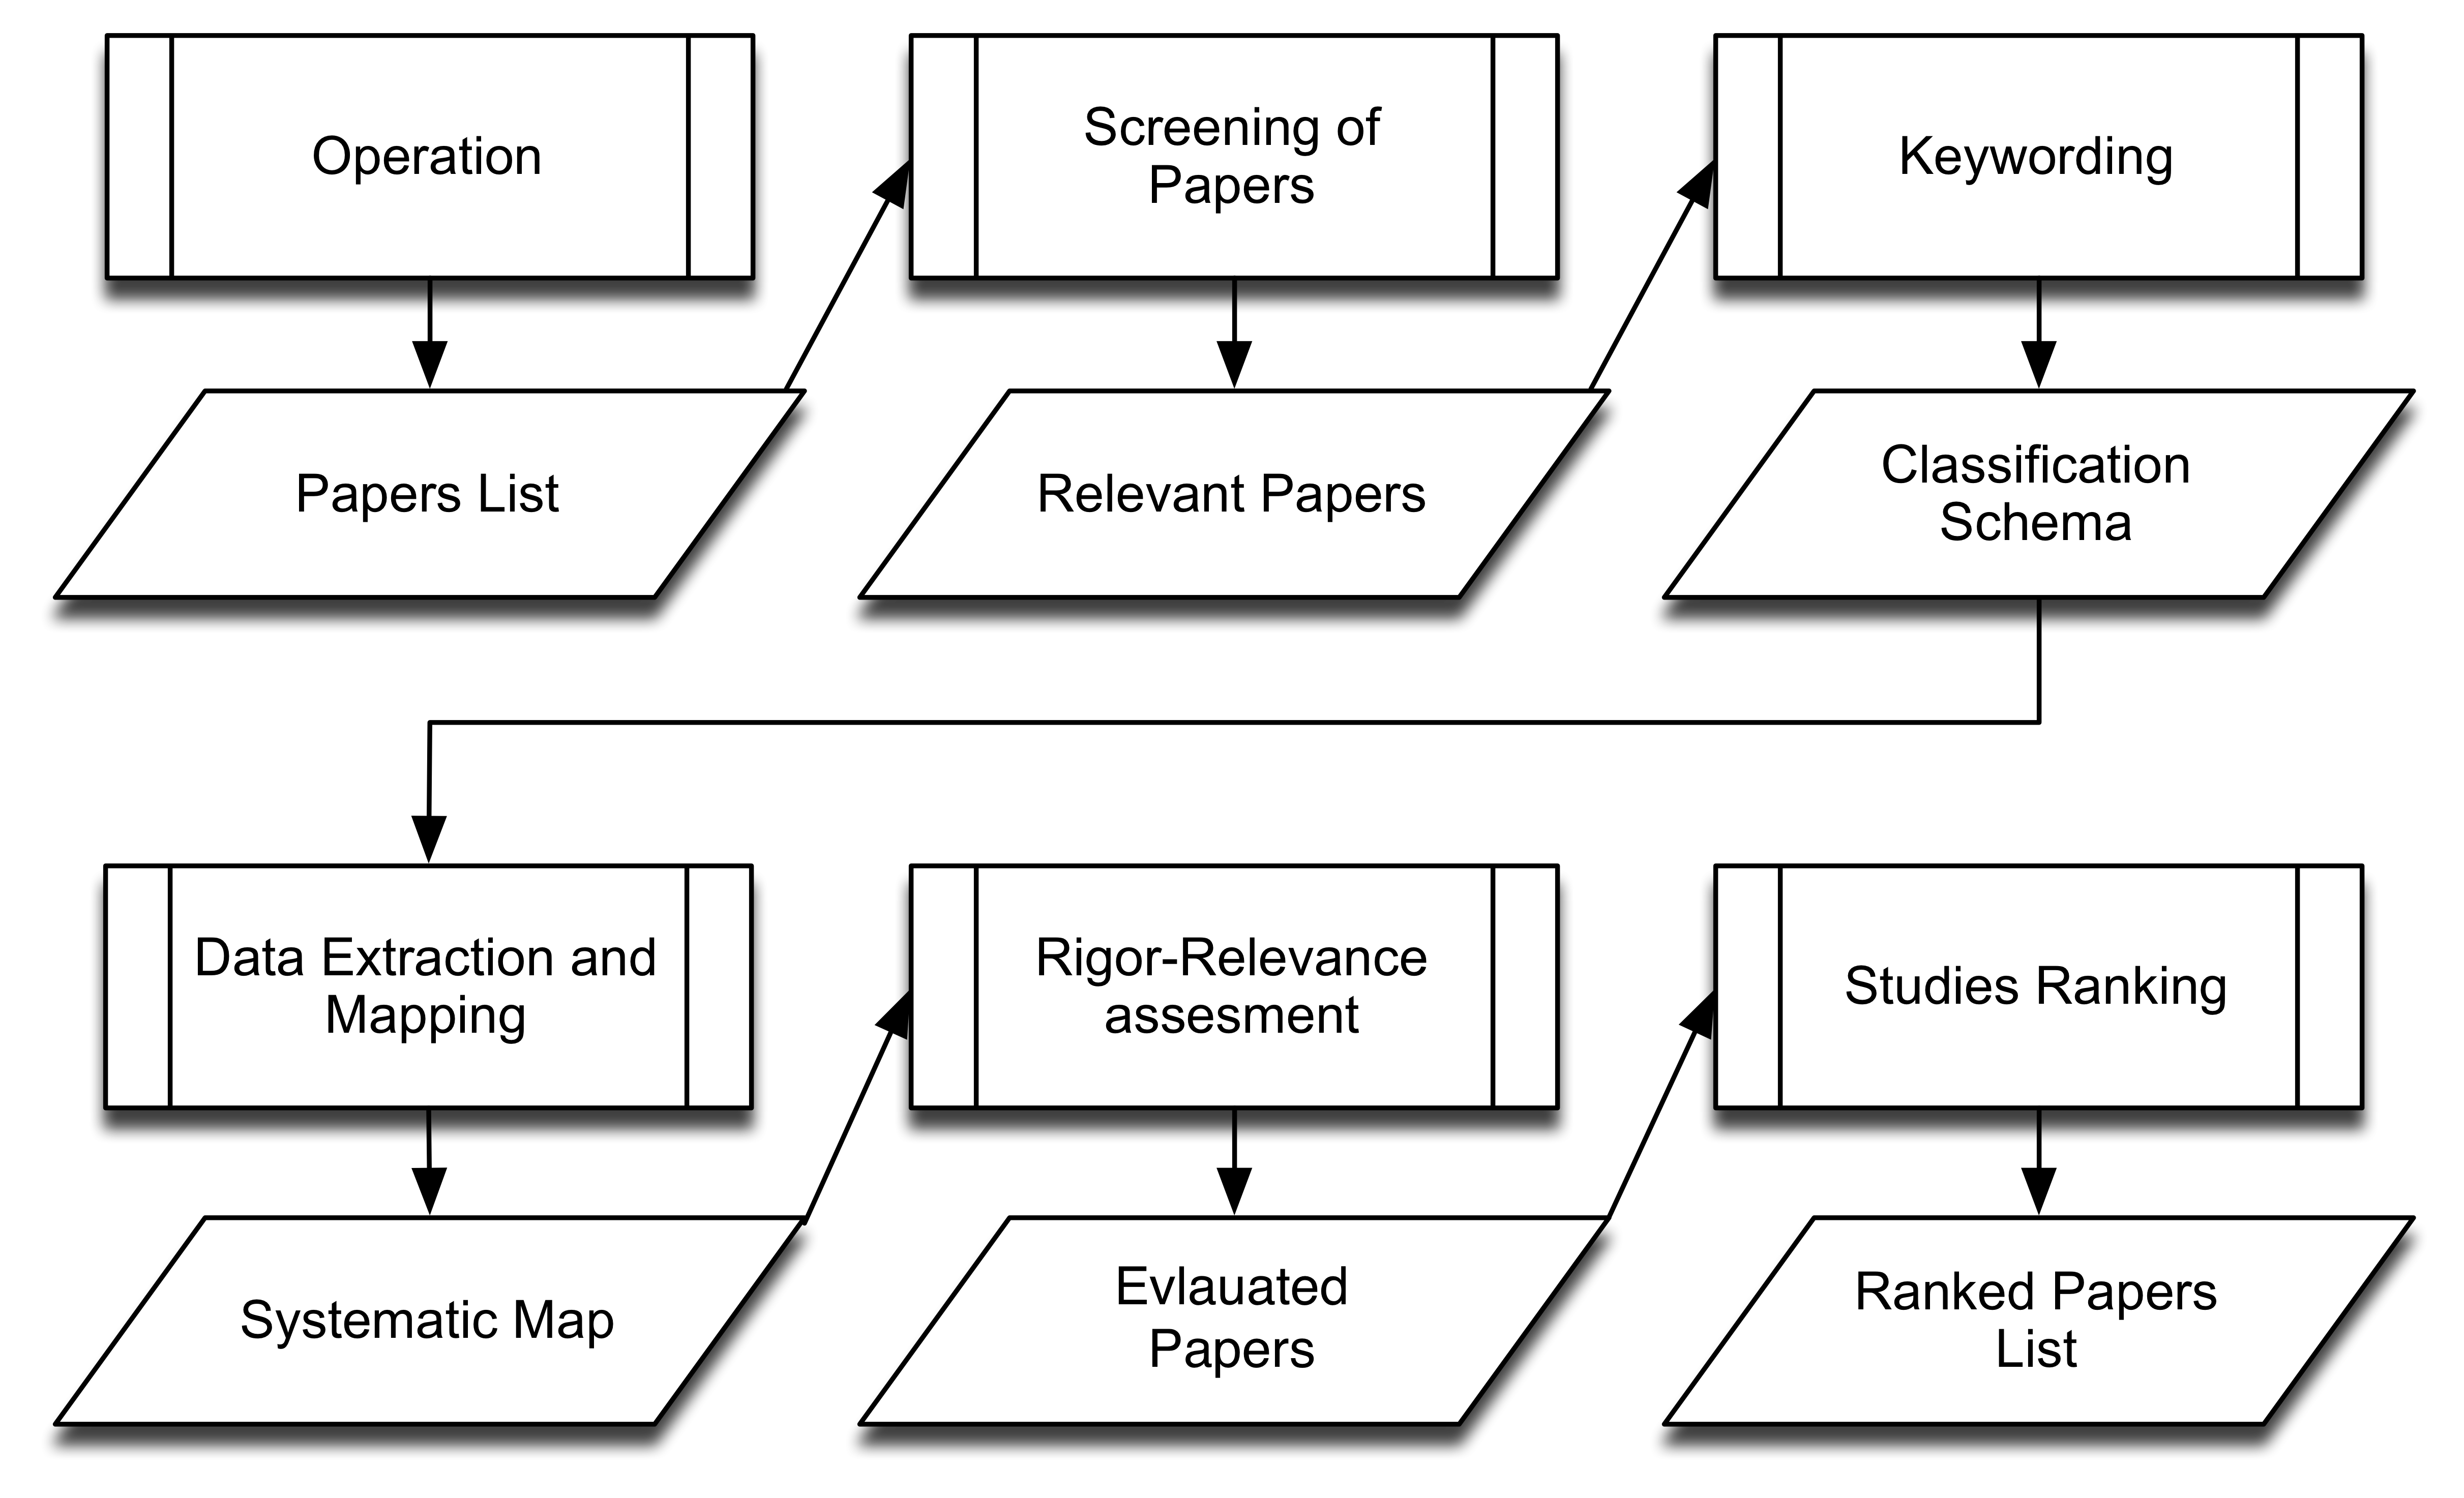
\includegraphics[width=0.5\textwidth,keepaspectratio=true]{figures/process_overview.png}
\caption{Process overview adapted from  \cite{Petersen2007}}
\label{fig:ms:sms}
\end{figure}
%%end figure


Starting from the research problem defined in \ref{sect:rm:rg}, the first step of our systematic study was  \textit{Operation}. The whole SMS procedure has been executed simultaneously in pair on the same screen, handling conflicts at the end of the \textit{data extraction and mapping} process by reviewing the rationale of similar decisions taken during the \textit{screening of papers}. When necessary we performed an in-depth review of the article\footnote{If the conflicts persisted after an in-depth review of the article, the third and fourth author of this paper... -/ take the final decision.}.

% subsection research_process_overview (end)

\subsection{Retrieving and screening  articles} % (fold)
\label{sub:retr_screen}

TThe first step for conducting a systematic search was iteratively building a \textit{search string} composed by different  \textit{keywords} that emerge by reviewing the scope of the research questions. To reflect our wide research problem we needed a very broad \textit{search string}, which was generated from three \textit{core concepts} identified as fundamental to our problem domain, i.e.:

\begin{itemize}

\item Software startup.
\item Development.
\item Process.
\end{itemize}


Following Rumsey’s guidelines \cite{how-find-information}, for each core concept we identified synonymous, related concepts, broader concepts, wider concepts, alternative spelling and part of speech that contributed to elaborate the list of terms included in our search string.

The second step was the identification of relevant and significant databases to include in our search process. To increase the internal validity of our research and the chances of finding relevant material we included in our target 5 of the most important peer-reviewed scientific online databases, namely:

\begin{itemize}

\item Compendex/Inspec \cite{compendex}.
\item ACM Digital Library \cite{ACMsearch}.
\item IEEE Xplore \cite{IEEExpl}.
\item ISI Web of Science \cite{ISIweb}.
\item Scopus \cite{scopus}.
\end{itemize}


To be more confident of the results, we included in the set of databases \textit{Google Scholar}  \cite{gScholar}, which indexes an extremely large set of data, both peer and non-peer reviewed. All the mentioned databases were selected in view of their ability to handle advanced queries.  

We then proceeded in customizing the \textit{search string} and iteratively perform the search while refining search \textit{keywords}. The overall process we used is shown in Figure \ref{fig:ms:conduct}.  

%%startFigure
\begin{figure}[H]
\centering
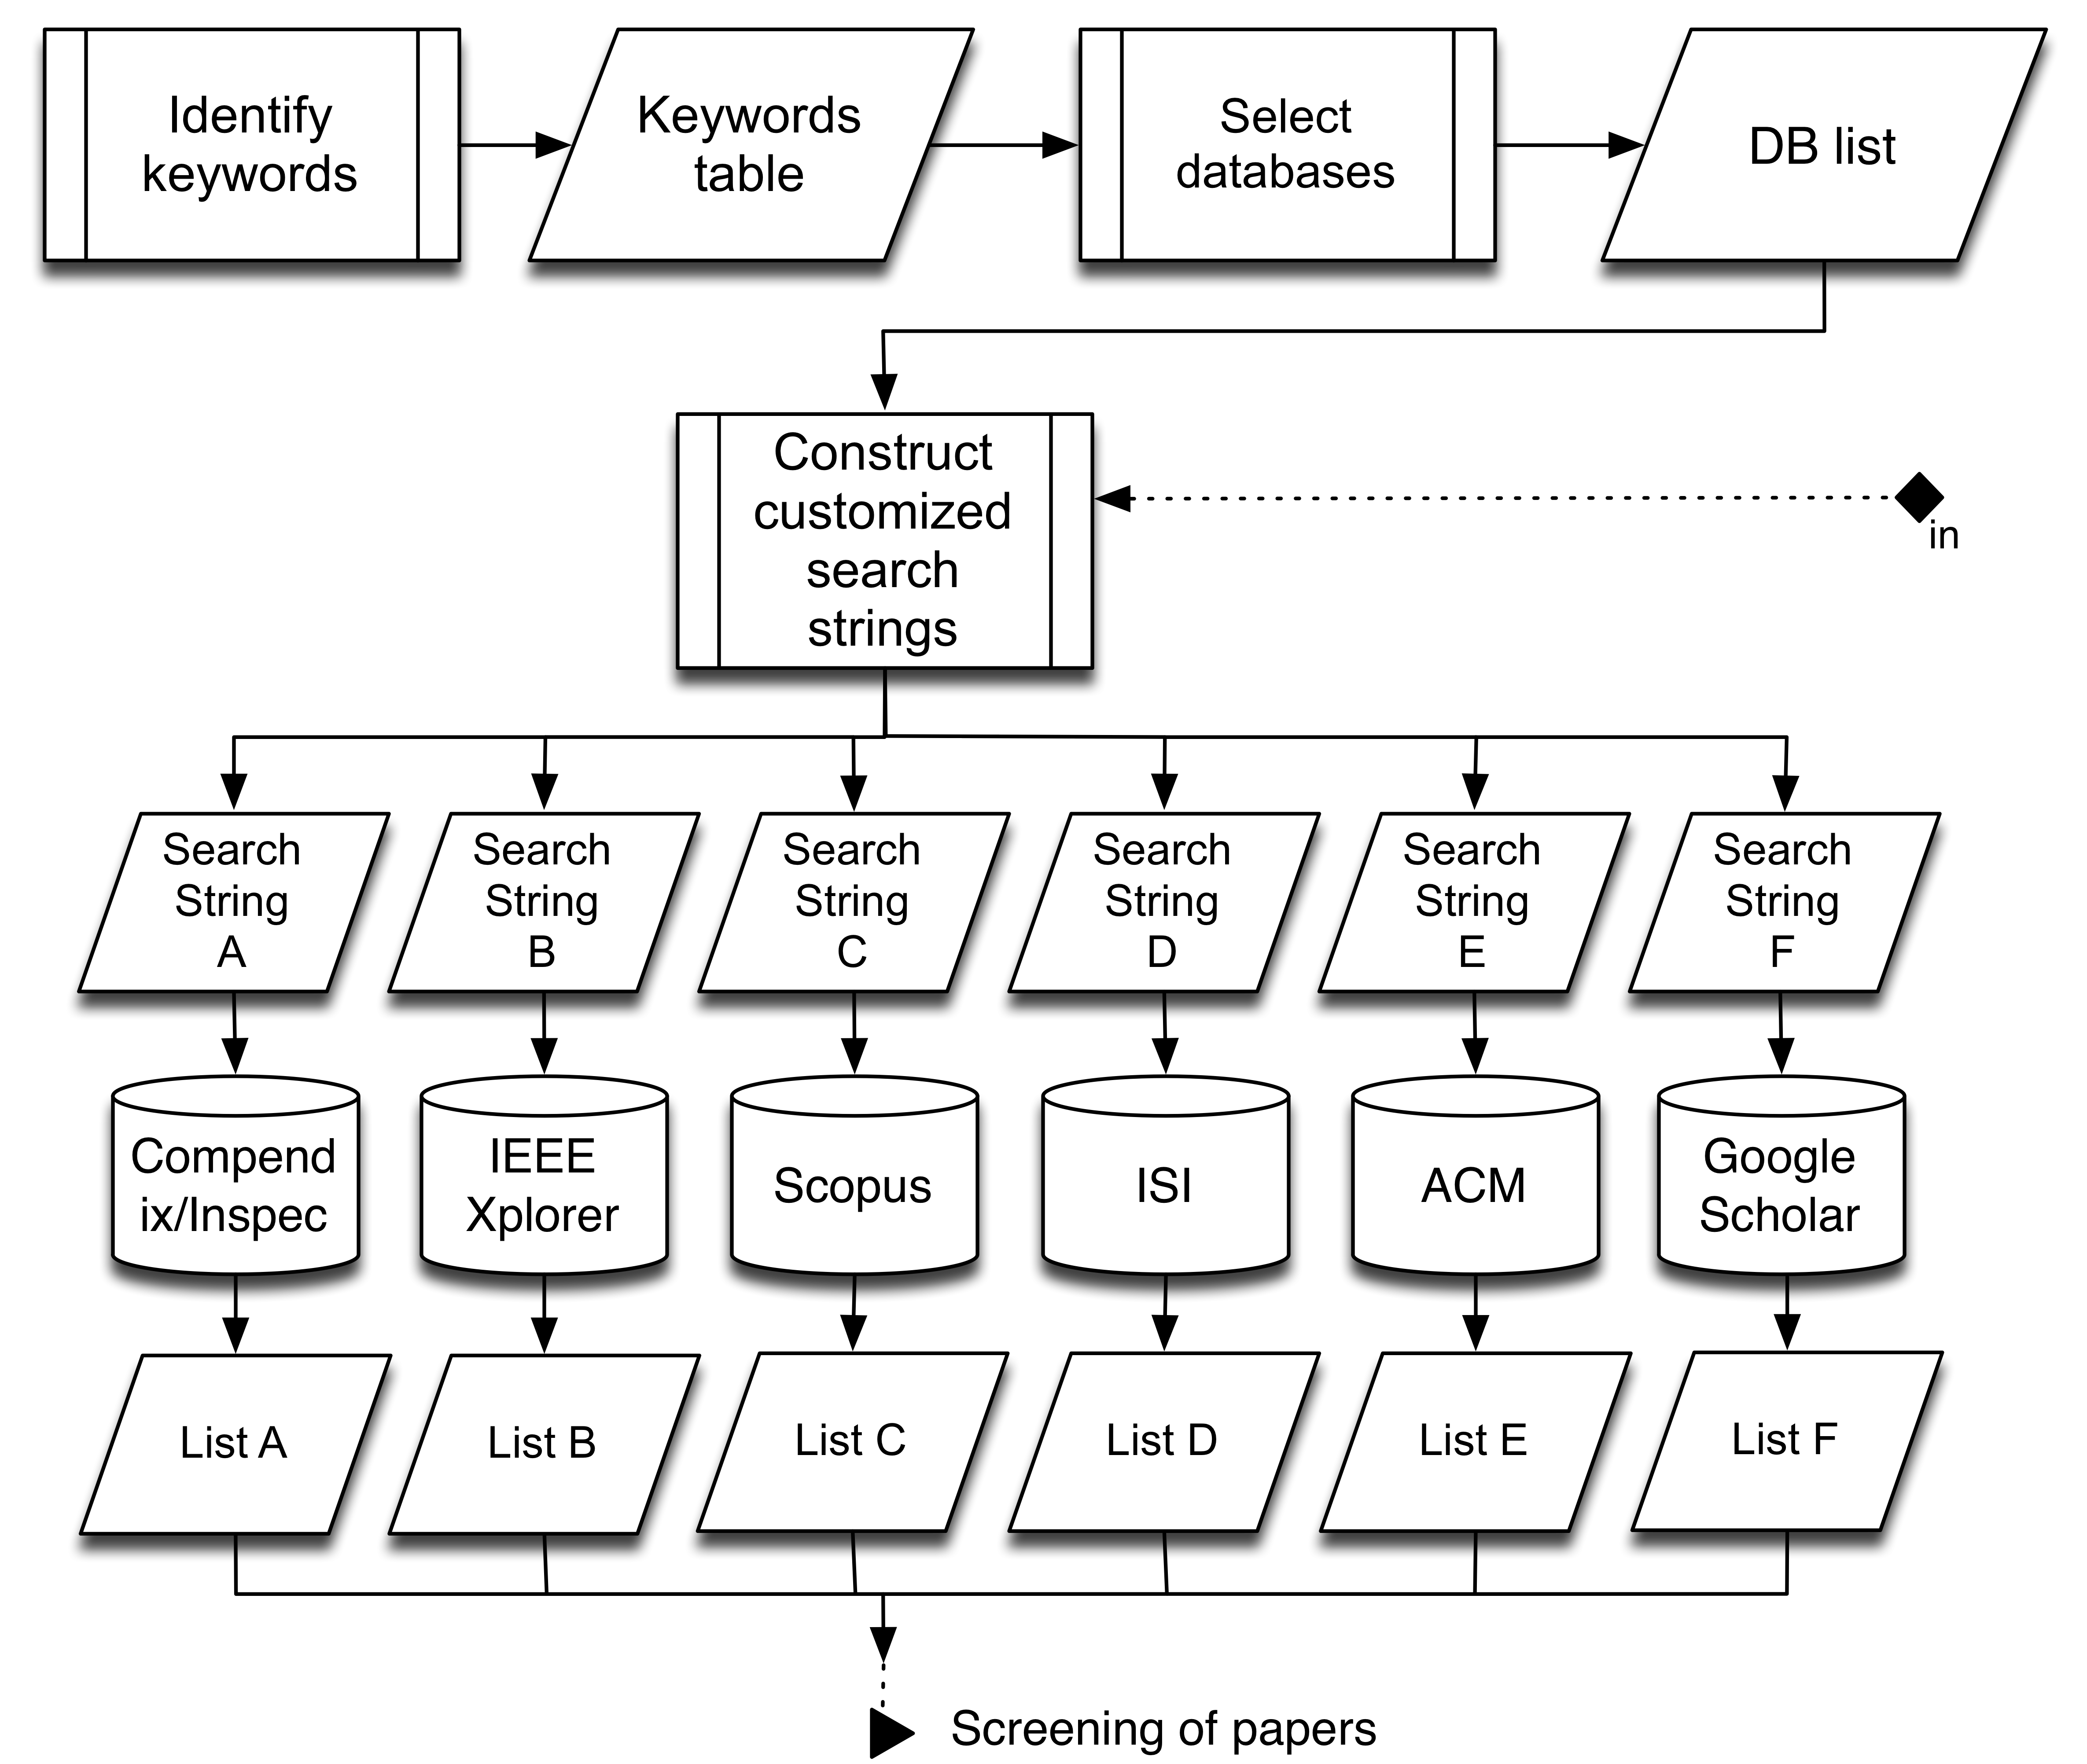
\includegraphics[width=0.5\textwidth,keepaspectratio=true]{figures/conduct.png}
\caption{Systematic Mapping Study - Operation }
\label{fig:ms:conduct}
\end{figure}
%%end figure


The procedure established in the figure above produces six different outputs - one per database - which are further analyzed as shown in Figure \ref{fig:ms:screening}.
The terms which formed our final search string are shown in Table \ref{tab:ms:search-keywords}, next to the core concept they represent\footnote{The symbol \textit{*} indicates the use a wildcard, mainly for including plural forms and alternative spellings.}. 

%Table of keywords  ---- ---- ---
\begin{table}[H]
\renewcommand{\arraystretch}{1.1}
\caption{Mapping Study - Search String Keywords}
\label{tab:ms:search-keywords}
\centering
\scriptsize \begin{tabular}{|p{0.75in}|p{1.7in}|}
\hline 
\hline
 Core Concept &	Terms \\
\hline
Software Startups & software startup*;  software start-up*; early-stage firm*; early-stage compan*; high-tech venture*; high-tech start-up*; start-up compan*; startup compan*; lean startup*; lean start-up*;  software package start-up*; software package startup*; IT start-up*; IT startup*; software product startup*; software start up*; internet start-up*; internet startup*; web startup*; web start-up*; mobile startup*; mobile start-up*;  \\ \hline 
Development & develop*; engineer*; model*; construct*; implement*; cod*; creat*; build*; \\ \hline 
Strategy & product*; service*; process*; methodolog*; tool*; method*; practice*; artifact*;  artefact*; qualit*; ilit*; strateg*; software; \\
\hline
\hline
 \end{tabular}
 \end{table}
%endtable

In forming our \textit{search string}, detailed in Appendix \ref{a:ms} (Table \ref{tab:ms:search-strings}), terms belonging to different core concepts were linked with the logical \textit{and},  while terms on the same row have been linked with the logical \textit{or}.

After executing the search strings on each database we saved the bibliographic references in 6 separated \textit{BibTeX} files, containing a total number of 1417 items, coming from different databases as shown in Table \ref{tab:ms:retrieved-overview}.

%table retrieved overview  ---- ---- ---
\begin{table}[H]
\renewcommand{\arraystretch}{1.1}
\caption{Retrieved papers source overview}
\label{tab:ms:retrieved-overview}
\centering
\scriptsize \begin{tabular}{|l|l|c|}
\hline 
\hline 
List & Database & Items   \\
\hline
List A & Inspec/Compendex & 508 \\
List B & IEEE Xplore & 104 \\
List C & Scopus & 357 \\
List D & ISI Web of Knowledge & 219 \\
List E & ACM Digital Library & 71 \\
List F & Google Scholar & 158 \\
\hline
      & \textbf{Total:} & \textbf{1417} \\
\hline
\hline 

 \end{tabular}
 \end{table}
%endtable


To execute the screening of papers we defined and followed a rigid step-by-step workflow, shown in Figure \ref{fig:ms:screening}. 

%%startFigure
\begin{figure}[H]
\centering
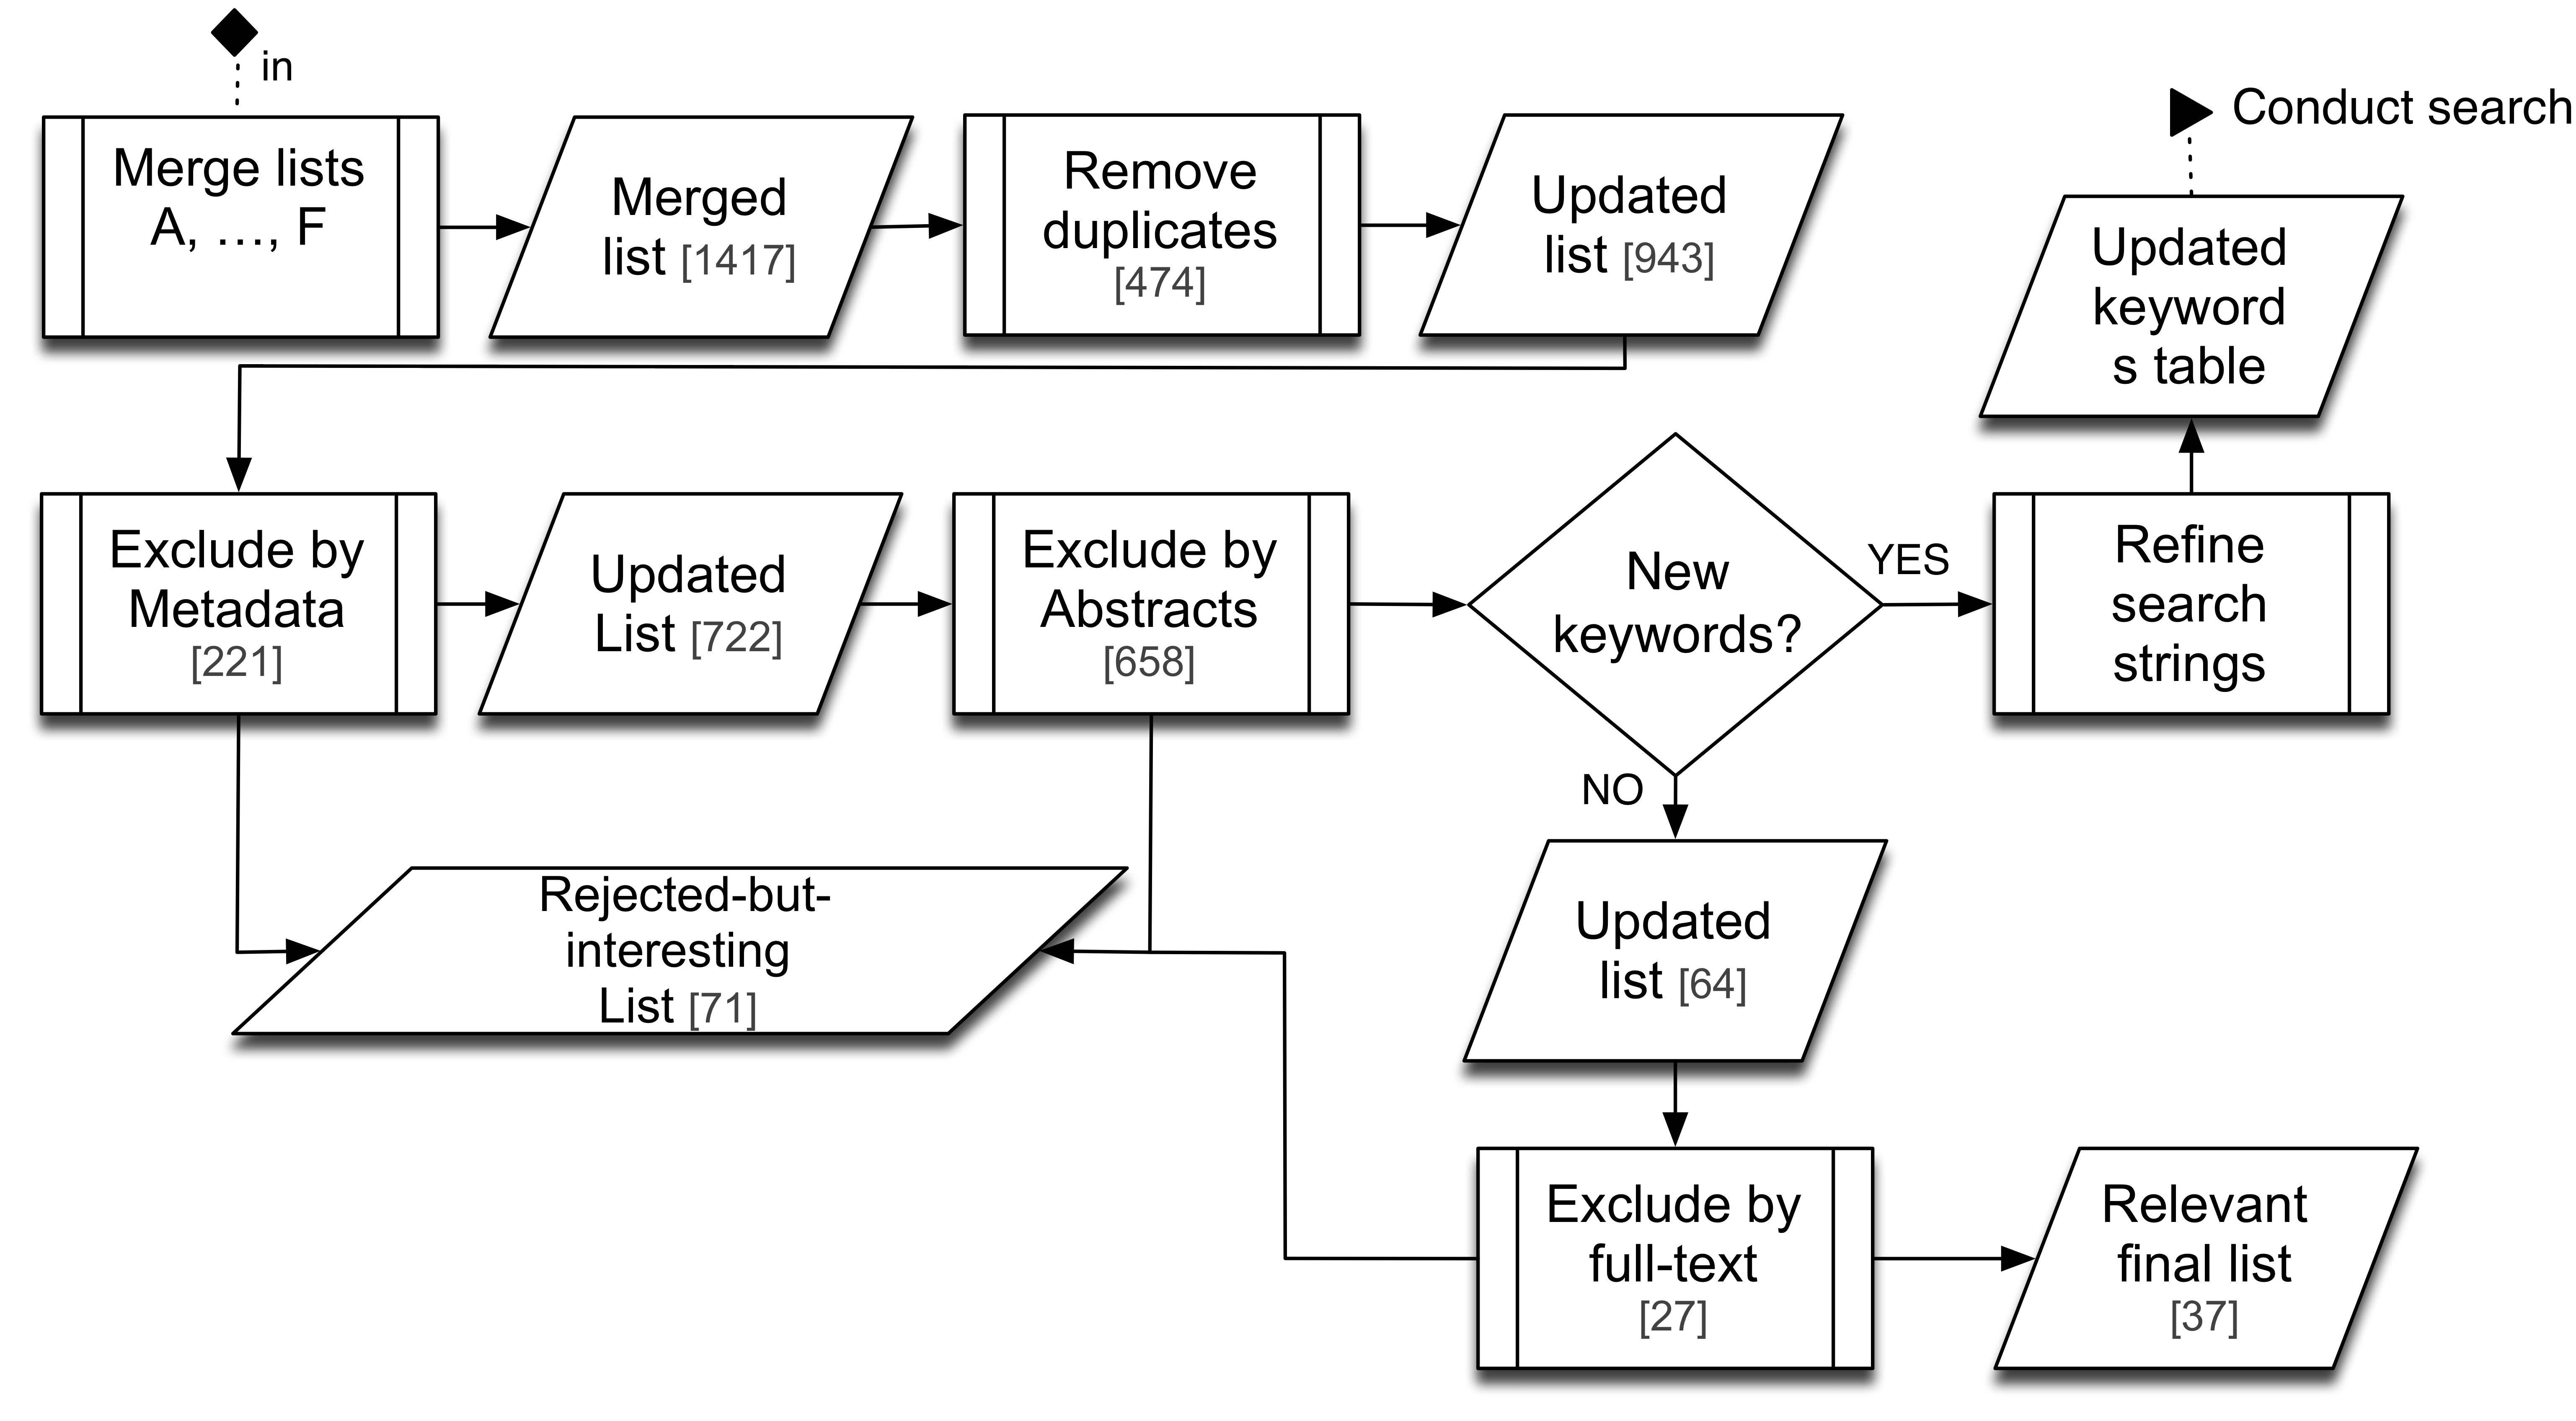
\includegraphics[width=0.5\textwidth,keepaspectratio=true]{figures/screening.png}
\caption{Screening of papers }
\label{fig:ms:screening}
\end{figure}
%%end figure

With the support of a tool for bibliographic management \cite{bibdesk} we merged the six lists together and removed the duplicate items in two distinct steps: first we used an automated feature to detect and remove items based on the author, year and title of the publication. Then, we manually deleted other duplicates that were not detected by the tool, for a total number of 474 duplicates.

Before proceeding with further exclusions we defined our \textit{inclusion/exclusion criteria}, aiming to include only peer-reviewed papers which brought some contribution to the body of knowledge of software engineering, by explicitly mentioning results related to software development in startups.
Additionally we decided to reject articles with the following characteristics:


\begin{itemize}

\item Non-peer reviewed (grey literature, books, \ldots).
\item Not written in English.
\item Clearly obsolete results (more than 20 years old).

\item Related to non-software companies (biotech, manufacturing, electronics, \ldots).
\item Related only to established companies (VSE, SME, research spin-offs).
\item Related only to technicalities of startups (algorithms, programming languages, \ldots).
\end{itemize}

We started analyzing the metadata of each article in pair (title, venue, keywords and the publication year) to exclude items that clearly didn’t satisfied the inclusion criteria (221), leaving important decision for the subsequent steps. Then, going through a more in-depth review, we analyzed abstracts of each paper to determine whether the article satisfied our inclusion criteria, eliminating 658 items. In case of internal conflicts, hard decisions, or incomplete abstracts we read through an entire article, excluding 27 additional items. As shown in Figure \ref{fig:ms:screening}, while screening abstracts we improved the search process by enriching the initial search strings with new keywords identified in retrieved articles and iteratively conducting a new search (Figure \ref{fig:ms:conduct}).

During the screening of papers, we have found that some articles, not included, had the potential of contributing to our analysis. For this reasons we created an additional list (\textit{Rejected-but-interesting List}) that we filled during the exclusion process with 71 managerial articles filtered and analyzed in a dedicated section in Appendix \ref{a:related:management}.


During this review process we kept track of the rationale for each exclusion, visually presented in the right column of the Figure \ref{fig:ms:exclusion}.

%%startFigure
\begin{figure}[H]
\centering
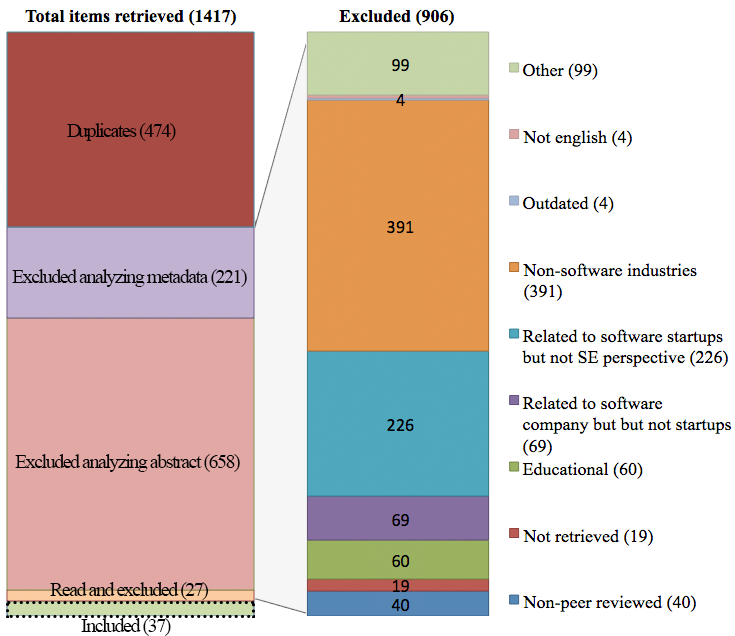
\includegraphics[width=0.5\textwidth,keepaspectratio=true]{figures/exclusion.png}
\caption{Studies selection process overview }
\label{fig:ms:exclusion}
\end{figure}
%%end figure

The majority of paper we excluded were not related to the software industry (391), not interesting under a SE perspective (226) or related to established companies (69). Other excluded work were off-topic (99), educational (60), non peer-reviewed (40), non-English(4) or outdated (4).  

% subsection retr_screen (end)

\subsection{Mapping} % (fold)
\label{sub:mapping}
//Distinguish between this keywords and terms of the search string!!
//Here specify how keywords have been extracted

To generate the \textit{classification schema} we used the technique of \textit{keywording}, following the systematic process illustrated in Figure  \ref{fig:ms:keywording}.

%%startFigure
\begin{figure}[H]
\centering
\includegraphics[width=0.5\textwidth,keepaspectratio=true]{figures/keywording.png}
\caption{Classification schema creation adapted from \cite{Petersen2007}}
\label{fig:ms:keywording}
\end{figure}
%%end figure

The first step consisted in reading abstracts of the relevant studies, assigning them a set of keywords, to spot the main contribution area of a paper. To get a rough understanding of the research area represented by the sample of collected papers, we combined together the defined keywords forming a high-level set of categories, which initially generated a first representation of the selected articles. Then, by progressively trying to fit the articles into categories, the schema underwent a refinement process by being updated to receive new data.

When executing the actual extraction, we motivated with comments the non-obvious decisions we took in a spreadsheet, writing the rationale behind the belonging of an article to a certain category rather than another. The output of this process is shown in \textit{Results and Analysis} (see Subsection \ref{sect:res:ms:rq1-1}) and represents the final \textit{systematic map}. 

% subsection mapping (end)

\subsection{Data extraction} % (fold)
\label{sub:data_extraction}

After we defined the \textit{classification schema} (presented in Subsection \ref{sect:res:ms:rq1-1})we proceeded to systematically extract data from the selected relevant studies.  We filled a spreadsheet where, for each article, we assigned a specific category of the \textit{schema}, and additionally we collected other information inspired by other similar studies \cite{Dyba2008, Shepperd2007}:

//Distinguish metadata and non-metadata
//Talk about themes and how we extracted them


\begin{itemize}

\item Article title.
\item First author.
\item Year of publication.
\item Synthesis of results (one-line).
\item Keywords.
\end {itemize}

We took advantage of the data extraction process to identify an additional relevant aspect which emerged while reading abstracts and documents:  the recurrent patterns of common attributes among startup companies (resulting \textit{themes} are reported in Subsection \ref{sect:res:ms:rq1-3}). Moreover, the bibliography of each extracted article has been screened to identify other possible relevant articles to our research, adopting the \textit{snowballing} technique\footnote{Note that in our case with snowball sampling we didn’t identify any additional relevant article, but in the case that relevant articles were retrieved, a refinement of keywords and reprocess of the \textit{systematic mapping study} would have been required as described in Figure \ref{fig:ms:conduct}.} \cite{snowballing}. 

//Data extraction we should add the content review we made by reading it



% subsection data_extraction (end)

\subsection{Rigor and relevance assessment} % (fold)
\label{sub:rigor_and_relevance}

The primary challenge of SE is to transfer research results and knowledge to practitioners showing valid and concrete advantages  \cite{Ivarsson2010}. To assess how results are presented in our studies’ selection, we integrated the traditional framework of SMS with an additional step, that is the evaluation of paper’s \textit{rigor} and \textit{relevance}.

We used a systematic and validated model developed by Ivarsson and Gorschek \cite{Ivarsson2010} to evaluate the scientific rigor and the industrial relevance of each paper. The model provides a complete set of rubrics to measure \textit{rigor} and \textit{relevance} dividing these two factors in different aspects, and quantifying the way in which each aspect is considered in the study (also see \cite{IvarssonGorsREj} for a real application).

As described by the authors, rigor refers to the precision or exactness of the research method used and how the study is presented. Aspects that are considered are:

\begin{itemize}

\item Context - description of development mode, speed, company maturity and any other important aspect where the evaluation is performed.
\item Study design - description of the variable measured, treatments, control used and any other design aspect considered.
\item Validity - description of different types of threats to validity evaluating conclusion, internal, external and construct validity.
\end {itemize}


On the other hand the relevance of an article consists of the realism of the environment where the study is performed and in the degree to which the research method undertaken has been investigated in several literature reviews. Aspects that are considered are:

\begin{itemize}

\item Subjects - use of subjects who are representative of the intended users of the technology.
\item Context - use of settings representative of the intended usage setting.
\item Scale - use of a realistic size of the applications.
\item Research method - use of a research method that facilitates investigating real situations and relevant for practitioners.
\end {itemize}

Aspects related to the rigor of the study are scored with three score levels: \textit{weak}, \textit{medium} and \textit{strong} description. Whilst, aspects related to relevance are scored 1 if contributing, 0 otherwise. For the sake of brevity we reported only the high-level quantification table (see Table \ref{tab:ms:quantific-relev-rig}). The detailed rubrics, used to evaluate the articles, can be found in \cite{Ivarsson2010}.

%Quantification of rigour and relevance  ---- ---- ---
\begin{table}[H]
\renewcommand{\arraystretch}{1.1}

\caption{Rigor and relevance quantification}
\label{tab:ms:quantific-relev-rig}
\centering
\scriptsize\begin{tabular}{|lc|}

\hline
\hline 
\multicolumn{2}{|l|}{ \textbf{Rigor} Ri =  Ri1 + Ri2 + Ri3} \\
\hline 
Context described (Ri1) &    \\
Study design described (Ri2) &    \\
Validity discussed (Ri3) &    \\
\hline
\multicolumn{2}{|l|}{Each aspect scored according to following scheme } \\ \hline
Weak presentation & 0 \\
Medium presentation & .5 \\
Strong presentation & 1 \\
\hline


\hline \hline


\multicolumn{2}{|l|}{ \textbf{Relevance}: Re =  Re1 + Re2 + Re3 + Re4} \\
\hline 
Context (Re1) &    \\
Research method (Re2) &    \\
User/Subject (Re3) &    \\
Scale(Re4) &    \\
\hline
\multicolumn{2}{|l|}{Each aspect scored 1 if contributing to relevance, 0 otherwise} \\ 
\hline
\hline

 \end{tabular}
 \end{table}
%endtable


Finally to obtain the final score of rigor and relevance the sum is performed according to the number of aspects that are classified as contributing to the industrial rigor and relevance respectively.

With this approach we intended to extend the scope of the traditional \textit{Systematic Mapping Study}, which is limited to paper classification without assessing the quality of underlying studies. In our research, by combining a classic SMS with the study of rigor, relevance and the creation of a simple ranking function (see next subsection), we obtained a quick tool to partially overcome the above-mentioned limitations.


% subsubsection rigor_and_relevance_assessment (end)


\subsection{Ranking of articles} % (fold)
\label{sub:ranking_of_articles}
The final step, which concludes the mapping study, is the creation of a ranking function. We assigned a score to each paper, evaluating it in face of its \textit{classification schema}’s categories, \textit{rigor} and \textit{relevance} score, and two additional factors which characterize the venue of the study and the publication year.

We provided a rough estimation of the actual \textit{value} that each paper brought to the research domain, by giving more importance to recent rigorous journal articles entirely devoted to the topic and presenting empirical results relevant to practitioners. To reflect those criteria, we used tables for converting each factor into an arbitrary numerical value in the range between 0 and 10. The conversion tables which were used to quantify the internal score of each dimension are discussed in Appendix \ref{a:ms:score-quant}. The final ranking of the 37 relevant articles is presented in \textit{Results and analysis} (see Subsection \ref{sect:res:ms:summary}).


//Maybe add tables with  scores motivation?
% subsection ranking_of_articles (end)



\subsection{Threats to validity} 
 \label{sub:validity}

We identified potential threats to the validity of the systematic mapping and its results, which are presented in this section together with the mitigation strategies, structured following the example of  a recent study \cite{Unterkalmsteiner2012}.

%--------------------------%%--------------------------%%--------------------------%%--------------------------%%--------------------------%%--------------------------%%--------------------------%
\subsubsection{Publication bias}
\label{sect:rm:ms:validity:pub}

Systematic reviews suffer from a common bias due to the general problem that \textit{positive outcomes are more likely to be published than negative ones}  \cite{Unterkalmsteiner2012}.
In our study this threat is moderate, since the conclusions we draw and the \textit{theoretical framework} we present are based on empirical data. The literature review is only used to make a comparison and validation of our results.
%--------------------------%%--------------------------%%--------------------------%%--------------------------%%--------------------------%%--------------------------%%--------------------------%
\subsubsection{Threat to identification of primary studies}
\label{sect:rm:ms:validity:thre}

The approach we used to construct the \textit{search string} (see Section \ref{sect:rm:ms:conduct}) aimed to collect the larger number of articles related to software development in startups as possible.

However, a limitation of the current search string lies in the non-inclusion of the stand-alone terms \textit{``startup''} or \textit{``start-up''}, to avoid the screening of more than 20 thousands papers, mostly irrelevant because related to the english phrasal verb ``to start up'', largely used in many disciplines to indicate the commencing moments of an engine. Then, to mitigate the risk of losing some relevant articles, we included in the search string many redundant terms in logical \textit{or}, to increase the chances of catching any paper somehow related with software development in startup companies limiting the risk of obtaining an unreasonable number of articles with an extremely low \textit{precision} (defined as the ratio of retrieved relevant and all retrieved \cite{Saracevic1995}) .

Considering the precision rate of the current \textit{search string} (3.92\%), the value we obtained is very low anyway, with 37 studies selected from an initial sample of 943.  However we were not interested in obtaining high precision as much as we wanted to obtain an high \textit{recall}, that is the expressed by the ratio of retrieved relevant articles and the existing relevant items \cite{Saracevic1995}.  Despite the recall is based upon an unknown quantity hard to estimate (especially in an area where no systematic reviews have ever been conducted to the best of our knowledge), to have our evaluated and validated relevant list we submitted our systematic review results to prominent researchers in the area (identified with the mapping study itself) immediately after executing the methodology. The risk of leaving out relevant results is further mitigated by the use of multiple databases, which cover the majority of scientific publication in the field.

We were not able to retrieve 19 items since they were not available neither in online catalogs nor in the three libraries we consulted. However, this is a minor risk as we had access to their titles, keywords and venues, which gave us a good degree of confidence they were not relevant. Additionally, considering our 3.92\% precision rate, the number of relevant articles in this small sample would have been statistically around \textit{one}.

Another threat was given by the fact that relevant studies could have been published after the actual execution of the systematic review. To mitigate this risk we used the alerts featured on \textit{Engineering Village} and \textit{Google Scholar} database which allowed us to receive a weekly newsletter with new items targeted by our \textit{search string}. At the current date (29th October 2012) no new relevant studies emerged.

Furthermore we noticed a high inconsistency in the use of the word \textit{startup} by different researchers, even in the same area. We couldn’t identify a single and widely accepted definition of \textit{startup}, but we identified multiple and somewhat conflicting definitions. With the support of thesaurus and librarians specialized in software engineering we considered their suggestions for additional improvements.  Under these conditions, the attempt to identify a body of knowledge and restrict the scoping of our research was highly challenging. However, with the systematic study we were able to get a complete overview of how the term is used and sometimes misused, so we could focus the remains of our research on the early stage of startup companies, that is the most neglected stage by empirical primary studies so far.

Since startups and entrepreneurship in general are appealing for many sectors of the economy, an additional threat lies in the fact that some relevant information can be found in other academic sectors not considered in this systematic review.
%--------------------------%%--------------------------%%--------------------------%%--------------------------%%--------------------------%%--------------------------%%--------------------------%
\subsubsection{Threats to study selection and data extraction}
\label{sect:rm:ms:validity:sele}

An important bias to consider - as discussed in \cite{Dyba2008} - is related to the selection of publications and the data extraction process, that in our case has been mitigated with an up-front definition of the inclusion/exclusion criteria \cite{Kitchenham2007}. The extent to which a SMS is able to provide an overview of software engineering topics has been sufficiently reported by the comparison analysis with the systematic literature review, discussed in \cite{Petersen2007}.

The selection of relevant articles can be further biased by the personal opinions of researchers executing the process. To mitigate this threat and partially supply to our junior experience, we defined and documented a rigid protocol for the selection of each paper and we collaborated to mutually adjust each other biases by conducting the selection together and dedicating a reasonable amount of time to review conflicts, as suggested by \cite{Kitchenham2007}. Furthermore we documented the rationale behind the exclusions, to support us in the process of consensus creation by coherently consulting the history of previously taken decisions.

Another threat is related to researchers’ personal judgments, which can interfere with the evaluation of rigor and relevance of selected studies. However, the model we used to perform the assessment \cite{Ivarsson2010} provides rigorous guidelines and detailed rubric tables which have been observed to express our judgment more objectively.

An additional threat can undermine validity of the \textit{ranking} of selected studies (see Section \ref{sect:rm:ms:ranking}) that we computed, as the scores for each category and the weights for each dimensions have been arbitrarily chosen to reflect our criteria. However, we consider this threat marginal as we didn’t draw any important conclusions based on the ranking table and we specified that the score assigned to each paper has been used only to sort lists of relevant studies in the tables along the document. Furthermore we used an automatic spreadsheet to compute the final scores, which allowed us to adjust scores and weights, observing the effect of the final ranking in real time. For validating our ranking, we tried to modify scores/weights values several times, and we observed that the final ranking was not significantly altered by reasonable numerical adjustments, as long as we kept the order of importance between concepts.

Additionally, we used multi-methodological triangulation \cite{Wood,Kasunic2005} to confirm the validity of our results, by intersecting the data extracted with \textit{systematic mapping study} to the empirical data which we obtained by \textit{semi-structured interviews} and \textit{follow-up questionnaires}. 

 
 % subsection subsection_name (end)

\section{Classification schema} %-------- ## ----------------- ## ----------------- ## ----------------- ## ----------------- ## ---------
 \label{sect:schema}

 The above identified keywords, together with existing taxonomies, contributed to the formation of a formal \textit{classification schema}. The final schema, which emerged from the process specified in Subsection \ref{sect:rm:ms:extraction}, consists of four dimensions or \textit{facets}:

\par\vspace {0.4cm}
\begin{itemize}

\item \textit{Research type}: to represent the type of study undertaken.
\item \textit{Focus}: to describe the main focus of the research.
\item \textit{Contribution type}: to map the different types of outcome of the study.
\item \textit{Pertinence}: to distinguish between articles entirely devoted to engineering activities in startups and the ones which are only mentioning something related to it.
\end{itemize}
\par\vspace {0.4cm}

Each facet is formed by different categories described in the following four tables - one per dimension - which were used to map the selected studies and obtain a systematic map of the area.



The first dimension,  \textit{Research type} facet (see Table \ref{tab:ms:class-schema-res}), can be used to distinguish between different types of studies abstracting from the specific underlying research methodology, unlike other types of classification \cite{Ivarsson2010}. The research types have been adapted from \cite{Wieringa:2005}. The second dimension describes the categories of the \textit{focus facet}, which were obtained by clustering together sets of keywords previously identified (see Table \ref{tab:ms:class-schema-focus}).

%%

We separated studies concerning software development practices from articles focused on the high-level process management. Furthermore we provide two additional categories to classify articles focused on specific \textit{tools and technologies} and more \textit{managerial/organizational} studies. The third dimension, \textit{Contribution facet}, is presented in Table \ref{tab:ms:class-schema-pert}.



Similarly to the taxonomy used in \cite{Shaw2003}, this facet expresses which kind of contribution a study brings to the fields. Contribution types can be divided in  \textit{weak} (\textit{advices and implications},  \textit{lesson learned},  \textit{tools} and  \textit{guidelines}) and \textit{strong} (\textit{theory}, \textit{framework/methods} and \textit{model}).
Finally the \textit{pertinence facet} (see Table \ref{tab:ms:class-schema-contrib}) helps in distinguish between studies fully pertaining to engineering activities in software startups (\textit{full} pertinence), studies partially focused on some engineering activities in startups (\textit{partial} pertinence), and finally studies only mentioning some relevant information pertained to software development in startups (\textit{marginal} pertinence).  


%%
\onecolumn
\begin{table}[H]
\renewcommand{\arraystretch}{1.1}
\centering
\scriptsize  
\begin{tabular}{|p{1.35in}|p{3.85in}|}
\hline 
\hline  
\multicolumn{2}{|c|}{\textbf{Research type Facet}} \\
 \hline  
 
Evaluation Research & Methodology is implemented in practice and an evaluation of it is conducted. That means, it is shown how the research is implemented in practice (solution implementation) and what are the consequences of the implementation in terms of benefits and drawbacks (implementation evaluation). This also includes to identify problems in industry. \\ 
Solution Proposal & A solution for a problem is proposed, the solution can be either novel or significant extension of an existing methodology. The potential benefits and the applicability of the solution is shown by a small example or a good line of argumentation.  \\   
Philosophical Papers & These papers sketch a new way of looking at existing things by structuring the field in form of a taxonomy or conceptual framework. \\ 
Opinion Papers & These papers express the personal opinion of somebody whether a certain technique is good or bad, or how things should been done. They do not rely on related work and research methodology. \\ 
Experience Papers & Experience papers explain on what and how something has been done in practice. It has to be the personal experience of the author. \\

\hline \hline 
 \end{tabular}
 \caption{Classification schema - Research type facet}
\label{tab:ms:class-schema-res}
\end{table}
\small




\begin{table}[H]
\renewcommand{\arraystretch}{1.1}
\centering
\scriptsize 
\begin{tabular}{|p{1.35in}|p{3.85in}|}
\hline \hline
\multicolumn{2}{|c|}{\textbf{Focus facet}} \\
\hline  
  Type &	Description \\
\hline
Software development & Engineering activities used to develop software. \\ 
Process management & Engineering activities used to manage the development activities. \\ 
Tools and technology & Instruments used to create, debug, maintain and support development activities. \\ 
Managerial/organizational & Aspects that are related to software development, by means of: resource management and organizational structure. \\ 
\hline \hline
 \end{tabular}
 \caption{Classification schema - Focus facet}
\label{tab:ms:class-schema-focus}
\end{table}
\small
%%



%%
\begin{table}[H]
\renewcommand{\arraystretch}{1.1}
\centering 
\scriptsize 
\begin{tabular}{|p{1.35in}|p{3.85in}|}

\hline \hline
\multicolumn{2}{|c|}{\textbf{Contribution facet}} \\
\hline 
Type &	Description\\
\hline  

Model & Representation of an observed reality by concepts or related concepts after a conceptualisation process. \\  
Theory & Construct of cause-effect relationships of determined results.  \\ 
Framework/Methods & Models related to constructing software or managing development processes. \\  
Guidelines & List of advices, synthesis of the obtained research results.  \\  
Lesson learned & Set of outcomes, directly analysed from the obtained research results. \\   
Advice/Implications & Discursive and generic recommendation, deemed from personal opinions. \\    
Tool  & Technology, program or application used to create, debug, maintain or support development processes. \\

\hline \hline 



 \end{tabular}
 \caption{Classification schema - Contribution  Facet}
\label{tab:ms:class-schema-contrib}
\end{table}
\small
%%



%%
\begin{table}[H]
\renewcommand{\arraystretch}{1.1}
\centering
\scriptsize 
\begin{tabular}{|p{1.35in}|p{3.85in}|}
\hline \hline
\multicolumn{2}{|c|}{\textbf{Pertinence Facet}} \\
\hline  
  Type &	Description\\
\hline
Full  & Entirely related (main focus) to engineering activities in software startups.   \\ 
Partial & Partially related to  engineering activities in software startups. Main research focus related to engineering activities. \\ 
Marginal &  Marginally related to engineering activities in software startups. Main research focus different from engineering activities. \\
\hline \hline 
 \end{tabular}
\caption{Classification schema - Pertinence  Facet}
\label{tab:ms:class-schema-pert}
 \end{table}
\small
%%




\twocolumn
%%

\section{Results} %-------- ## ----------------- ## ----------------- ## ----------------- ## ----------------- ## ---------
 \label{sect:results}
This section presents the results of the \textit{systematic mapping study}. From an initial sample of 943 articles, we selected 37 relevant studies pertaining engineering activities in startups.

The section is structured according to the RQ-1 and its sub-questions:

\begin{itemize}
\item Publication distribution (see Subsection \ref{sect:res:ms:rq1-1}).
\item Rigor and relevance (see Subsection \ref{sect:res:ms:rq1-2}).
\item Contextual features of startups (see Subsection \ref{sect:res:ms:rq1-3}).
\item State-of-the-art: summary (see Subsection \ref{sect:res:ms:summary}).
\end{itemize}

\subsection{Publication distribution} % (fold)
\label{sub:publication_distribution}

Figure \ref{fig:ms:year}  shows the frequency distribution of  the publication year, from 1994 to 2011. 

%%startFigure
\begin{figure}[H]
\centering
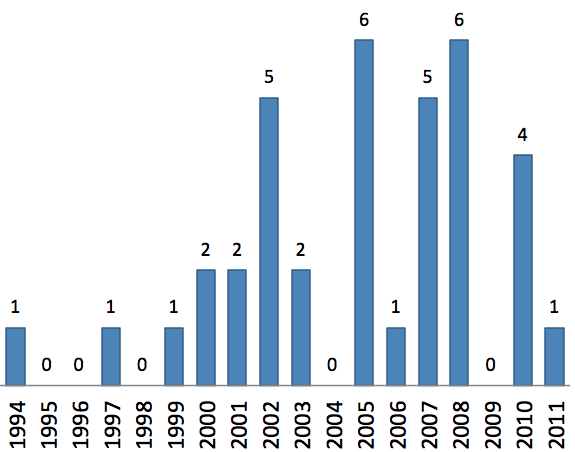
\includegraphics[width=0.5\textwidth,keepaspectratio=true]{figures/year.png}
\caption{Publication distribution-year}
\label{fig:ms:year}
\end{figure}

%%end figure 

To characterize what are the main topics covered within the area of engineering activities in software startups, we assigned to each article a set of keywords based on the content and the article’s own keywords (when available in the metadata), during the process of  \textit{keywording} (see Subsection \ref{sect:rm:ms:keywording}). From the 37 relevant studies we extracted a total number of 327 keywords (117 uniques) averaging about 9 keywords per article. To provide a visual representation of the content of the studies, we show the frequency of occurrence of each keyword in a \textit{tag-cloud} fashion\footnote{The tag cloud was generated with the online service (http://tagcrowd.com/).} in Figure \ref{fig:ms:cloud}. The table containing the raw data, which was used to generate it, is shown in Appendix \ref{a:ms} (see Table \ref{tab:ms:oneline}).

%%startFigure
\begin{figure}[H]
\centering
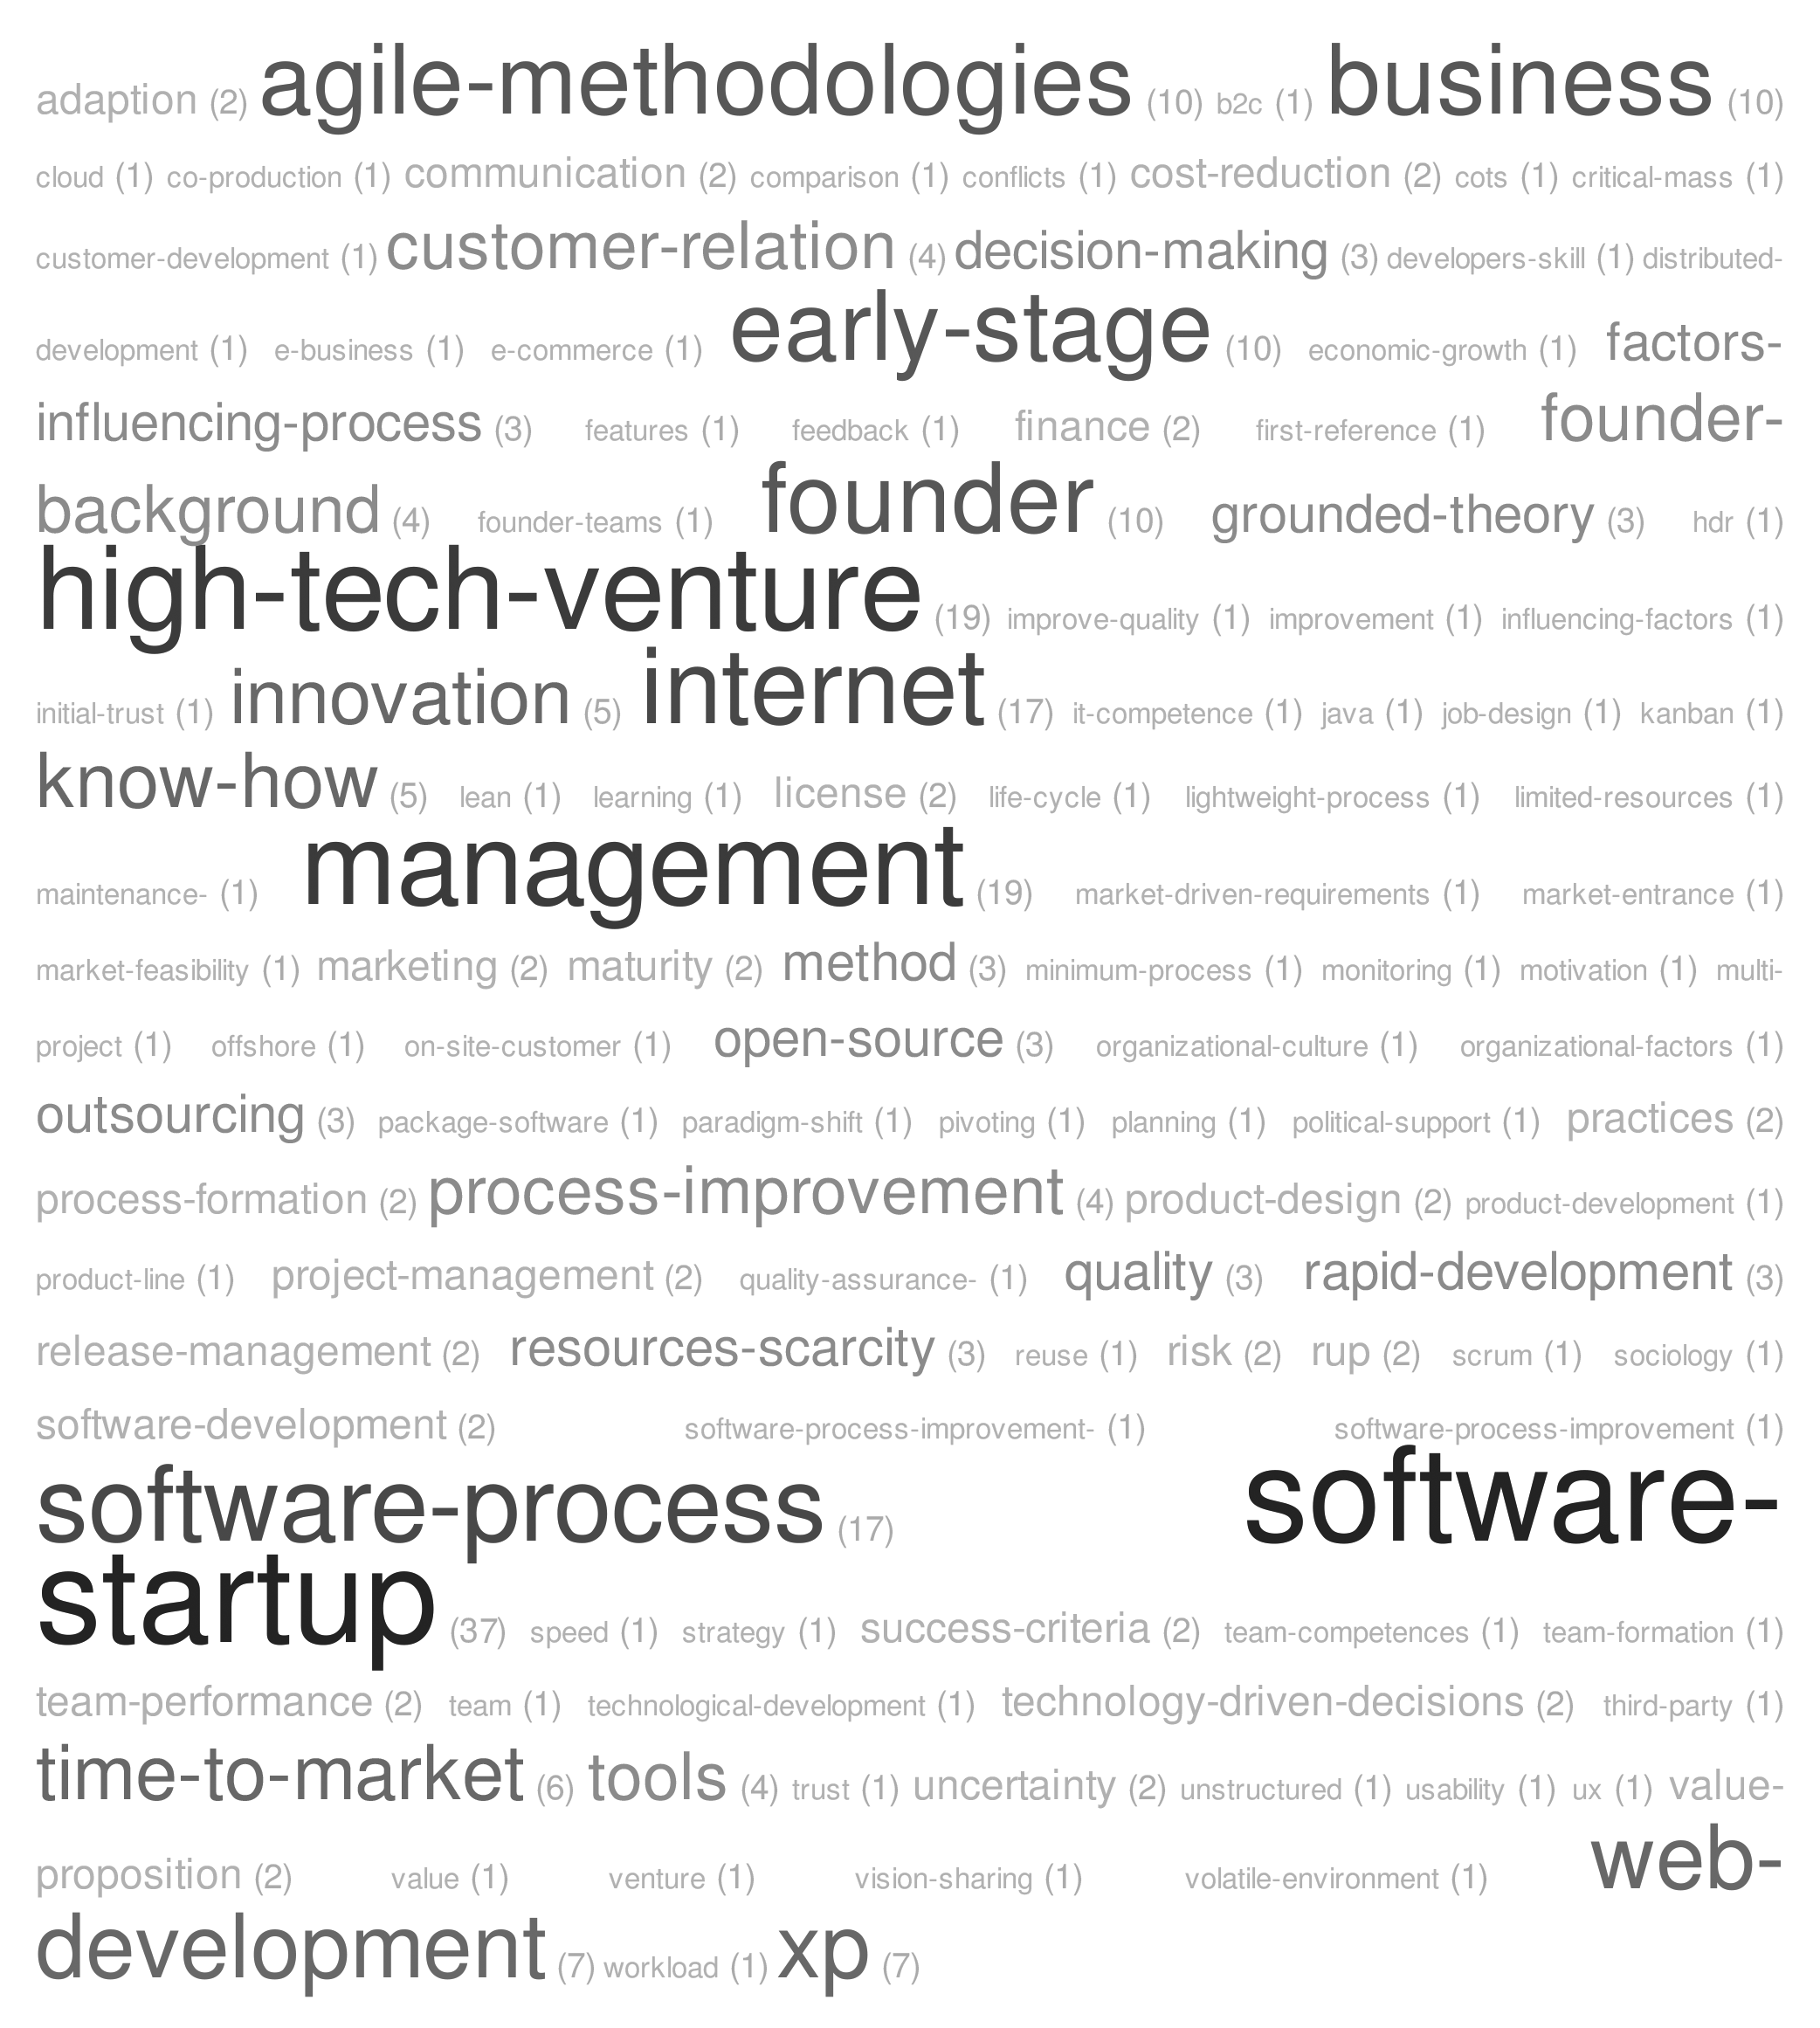
\includegraphics[width=0.5\textwidth,keepaspectratio=true]{figures/cloud.png}
\caption{Keywords cloud overview}
\label{fig:ms:cloud}
\end{figure}
%%end figure

The \textit{tagcloud} (see Figure \ref{fig:ms:cloud}) was obtained by assigning keywords to each study, reflecting the most important topics covered by the authors. Then, counting the occurrence of each keyword, the reader can grasp an overview of the main concern of the studies in the sample.

Furthermore, by reading the articles and analysing their references, we observed that the selected studies are poorly interconnected to each other. They represents low intra-referencing among authors which makes it harder to ground findings to existing works.	

Finally, by fitting the selected studies into the classification schema, we built the \textit{systematic map}, shown in Table \ref{tab:ms:refmap}.

%%
\onecolumn
\scriptsize 
{\begin{longtable}{|p{0.5in}|p{0.5in}|p{1.3in}|p{1.1in}|p{1.1in}|p{0.2in}|}
    \hline    \hline
     Author (year) &Pertinence  & Focus & Research Type & Contribution Type & Ref.  \\
    \hline   
    
\endfirsthead
	\multicolumn{6}{c}
	{\tablename\ \thetable\ -- \textit{Continued from previous page}} \\
   		\hline \hline
     		Author (year) &Pertinence  & Focus & Research Type & Contribution Type & Ref. \\
\hline
\endhead
\hline
\multicolumn{6}{c}
{\tablename\ \thetable\ -- \textit{Continued on next page}} \\
\endfoot
\endlastfoot


Coleman (2008) & Full  & Process Management & Evaluation Research & Model & \cite{Coleman2008} \\
Coleman (2007) & Full  & Process Management & Evaluation Research & Theory & \cite{Coleman2007} \\
Coleman (2008) & Full  & Process Management & Evaluation Research & Theory & \cite{Coleman2008a} \\
Kajko (2008) & Full  & Process Management & Evaluation Research & Model & \cite{Kajko-Mattsson2008} \\
H\"{a}sel  (2010) & Marginal & Managerial \& organizational & Evaluation Research & Model & \cite{Hasel2010} \\
Hanna (2010) & Marginal & Managerial \& organizational & Evaluation Research & Model & \cite{Hanna2010} \\
Deakins (2005) & Partial & Managerial \& organizational & Experience Paper & Model & \cite{Deakins2005} \\
Camel (1994) & Full  & Software Development & Evaluation Research & Lesson Learned & \cite{Camel1994a} \\
Silva (2005) & Full  & Software Development & Evaluation Research & Lesson Learned & \cite{Silva2005} \\
Midler (2008) & Partial & Managerial \& organizational & Evaluation Research & Framework \& Methods & \cite{Midler2008} \\
Taipale (2010) & Full  & Software Development & Experience Paper & Advice \& Implications & \cite{Taipale2010} \\
Chorev (2006) & Marginal & Managerial \& organizational & Evaluation Research & Model & \cite{Chorev2006} \\
Zettel (2001) & Full  & Software Development & Solution Proposal & Framework \& Methods & \cite{Zettel2001} \\
Jansen (2008) & Partial & Software Development & Evaluation Research & Lesson Learned & \cite{Jansen2008} \\
Sutton (2000) & Full  & Process Management & Opinion Paper & Advice \& Implications & \cite{Sutton2000} \\
Heitlager (2007) & Full  & Process Management & Solution Proposal & Tool  & \cite{Heitlager2007} \\
Tingling (2007) & Full  & Software Development & Evaluation Research & Advice \& Implications & \cite{Tingling2007} \\
Deias  (2002) & Full  & Software Development & Experience Paper & Advice \& Implications & \cite{Deias} \\
Stanfill (2007) & Marginal & Managerial \& organizational & Solution Proposal & Advice \& Implications & \cite{Stanfill2007} \\
Wood (2005) & Partial & Software Development & Experience Paper & Advice \& Implications & \cite{Wood2005} \\
Steenhuis (2008) & Marginal & Managerial \& organizational & Evaluation Research & Lesson Learned & \cite{Steenhuis2008} \\
Yogendra (2002) & Partial & Managerial \& organizational & Evaluation Research & Guidelines & \cite{Yogendra2002} \\
Ambler (2002) & Full  & Software Development & Experience Paper & Lesson Learned & \cite{Ambler2002} \\
Crowne (2002) & Full  & Software Development & Solution Proposal & Advice \& Implications & \cite{Crowne2002} \\
Mater (2000) & Partial & Managerial \& organizational & Evaluation Research & Model & \cite{Mater2000} \\
Kakati (2003) & Marginal & Managerial \& organizational & Evaluation Research & Model & \cite{Kakati2003} \\
Kuvinka (2011) & Partial & Software Development & Experience Paper & Advice \& Implications & \cite{Kuvinka2011} \\
Su-Chuang (2007) & Marginal & Software Development & Evaluation Research & Advice \& Implications & \cite{Su-Chan2007} \\
Sau-ling Lai (2010) & Marginal & Managerial \& organizational & Evaluation Research & Lesson Learned & \cite{Lai2010} \\
Mirel (2000) & Partial & Managerial \& organizational & Solution Proposal & Advice \& Implications & \cite{Mirel2000} \\
Himola (2003) & Marginal & Managerial \& organizational & Solution Proposal & Advice \& Implications & \cite{Hilmola2003} \\
Kim (2005) & Marginal & Managerial \& organizational & Evaluation Research & Model & \cite{Kim2005} \\
Wall (2001) & Partial & Software Development & Experience Paper & Advice \& Implications & \cite{Wall2001} \\
Yoffie (1999) & Marginal & Managerial \& organizational & Evaluation Research & Guidelines & \cite{Yoffie1999} \\
Bean (2005) & Marginal & Tools and technology & Philosophical Paper & Advice \& Implications & \cite{Bean2005} \\
Tanabian (2005) & Marginal & Managerial \& organizational & Opinion Paper & Advice \& Implications & \cite{Tanabian2005} \\
Fayad (1997) & Marginal & Process Management & Philosophical Paper & Advice \& Implications & \cite{Fayad1997} \\

    \hline \hline

 \caption{ Systematic map overview }\label{tab:ms:refmap}\\
\end{longtable}}


\twocolumn
\small
%%


The above table quickly reveals the nature of the study conducted, the extent of pertinence with the research problem, the type of contribution produced and the major research area investigated. Although the table is complete and contains the entire classification schema, it is still hard to extract relevant information from it. For this reason we computed the frequency of publications in each category using an electronic spreadsheet. In this way it is easier to emphasize what has been achieved in the past by researchers in the area, identifying gaps to drive the direction of our \textit{grounded theory} case study, and suggesting possible future researches.

As suggested by Peterson et al. \cite{Petersen2007}, to provide a good overview on how the topic is structured, we present our \textit{systematic map} using multi-dimensional bubble charts (\textit{``x-y scatter plots with bubbles in categories intersections''}) where the size of the bubble is determined by the number of publications corresponding to the \textit{x-y} coordinates. Differently from other similar studies \cite{Smite2009,Dyba2006}, in our \textit{classification schema} each data point is represented by four features. Thus, we created three plots to visualize all the six possible combinations of \textit{facets}, giving a complete overview of the systematic map.

For example, the big bubble in the top-left part of Figure \ref{fig:ms:fcr} indicates that 11 studies (29.73\% of the total) are focused on \textit{managerial and organizational factors} and conducted through an \textit{evaluation research}. Simultaneously in the same figure is possible to observe, for instance, how 7 items with \textit{managerial and organizational} focus contributed to the body of knowledge with a \textit{model}. However, by looking at Figure \ref{fig:ms:cpr}, one can quickly notice that 5 out of the total 9  \textit{models} have  only a \textit{marginal} pertinence with engineering activities in software startups.


\onecolumn
%%startFigure
\begin{figure}[H]
\centering
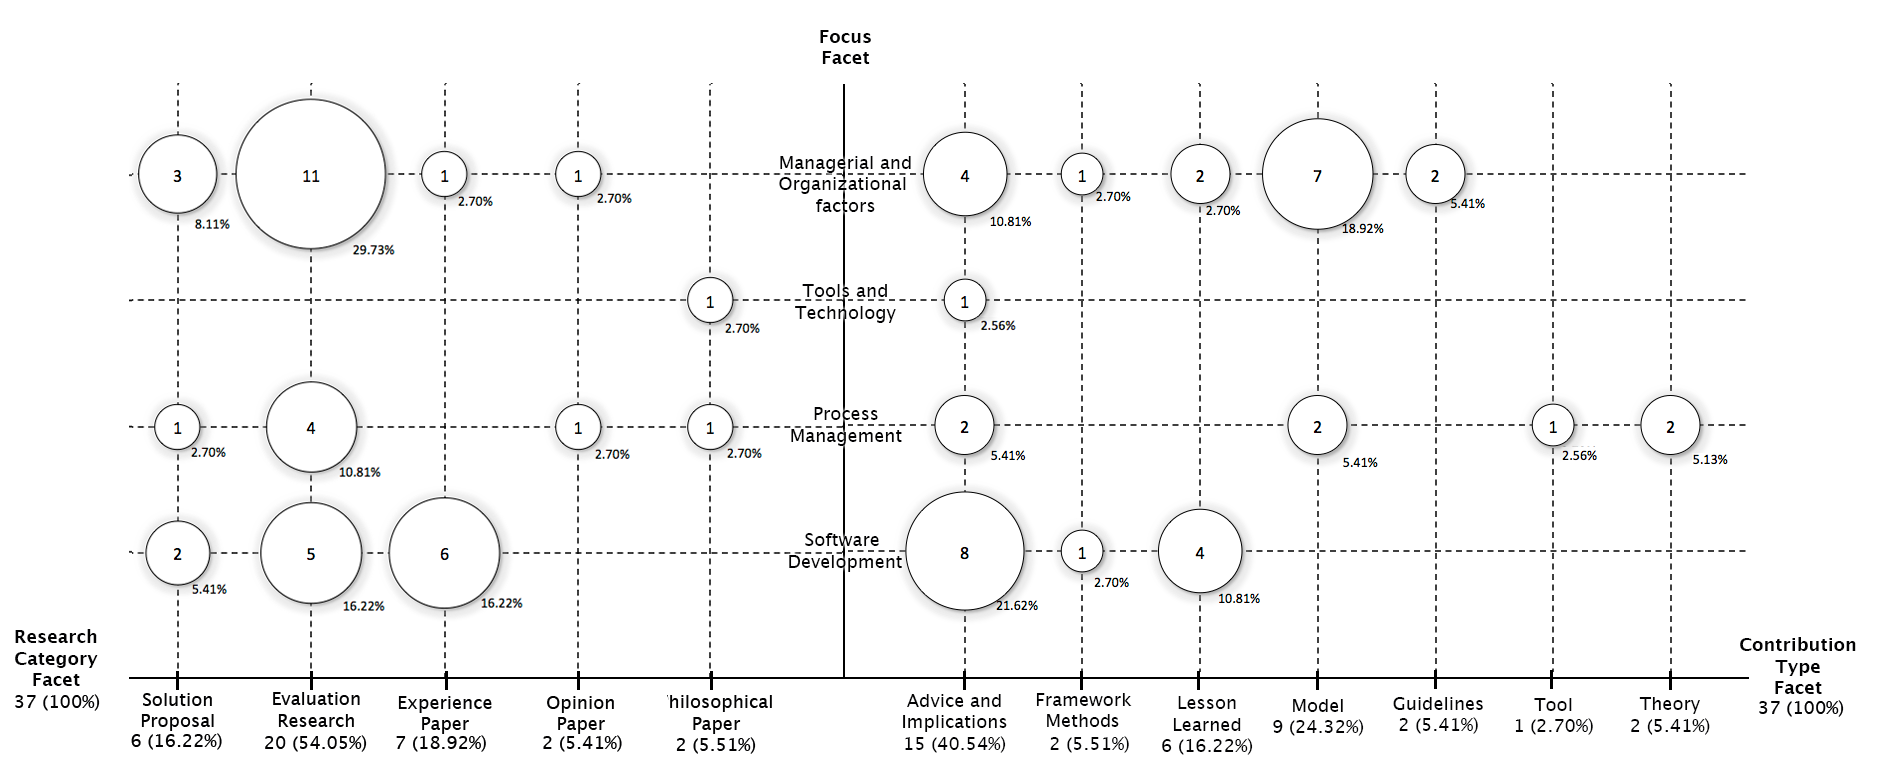
\includegraphics[width=0.8\textwidth,keepaspectratio=true]{figures/FCR.png}
\caption{Systematic map - \textit{Focus}, \textit{contribution} and \textit{research type}}
\label{fig:ms:fcr}
\end{figure}
%%end figure


 %%startFigure
\begin{figure}[H]
\centering
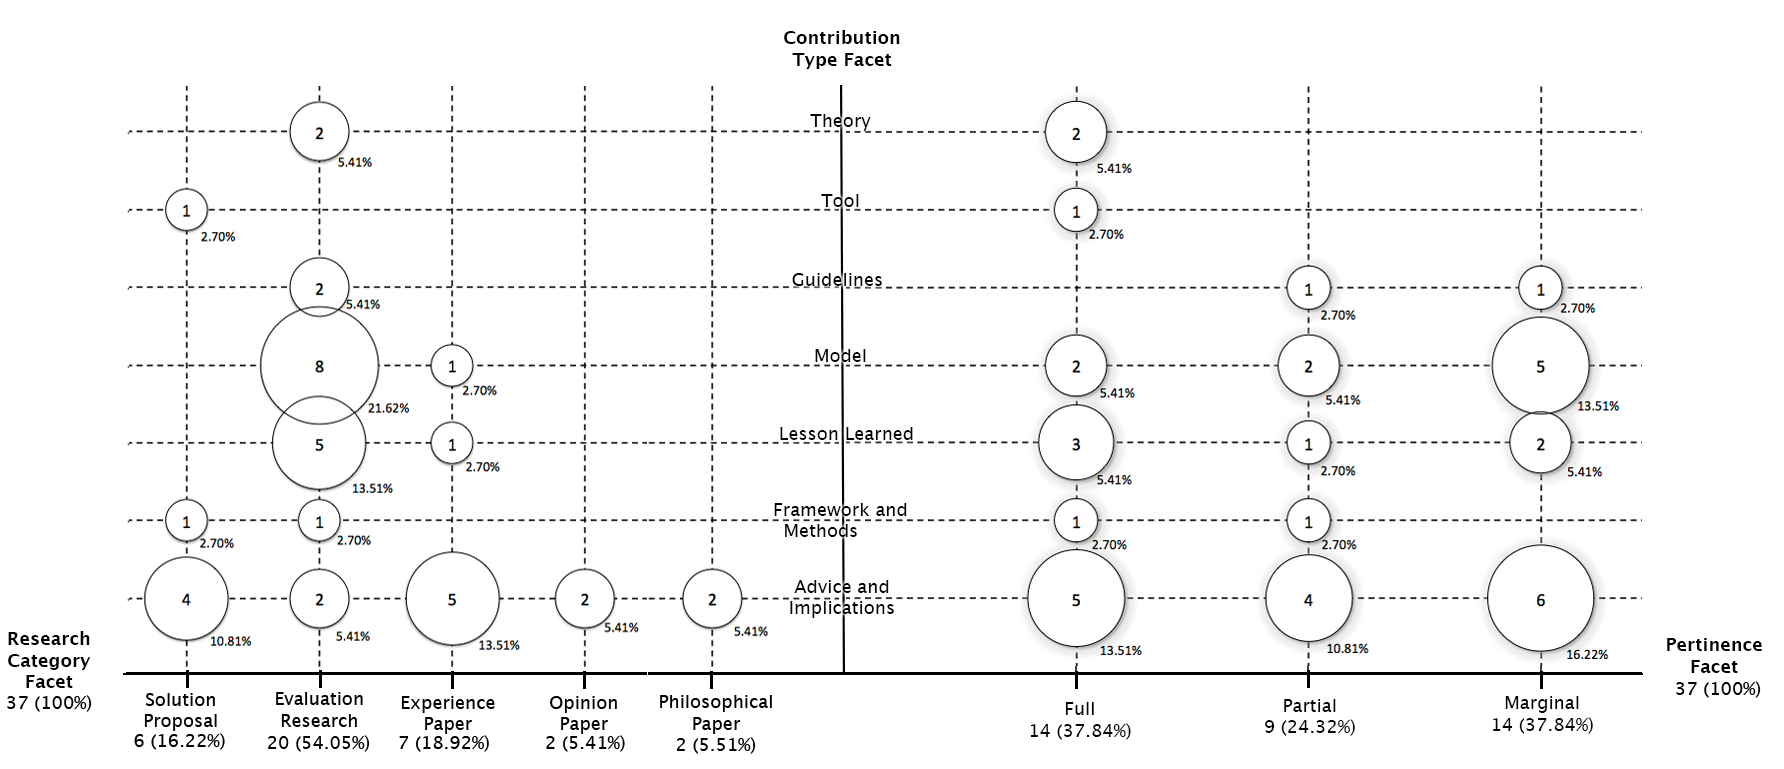
\includegraphics[width=0.8\textwidth,keepaspectratio=true]{figures/CPR.png}
\caption{Systematic map - \textit{Contribution}, \textit{pertinence} and \textit{research type}}
\label{fig:ms:cpr}
\end{figure}
%%end figure


 %%startFigure
\begin{figure}[H]
\centering
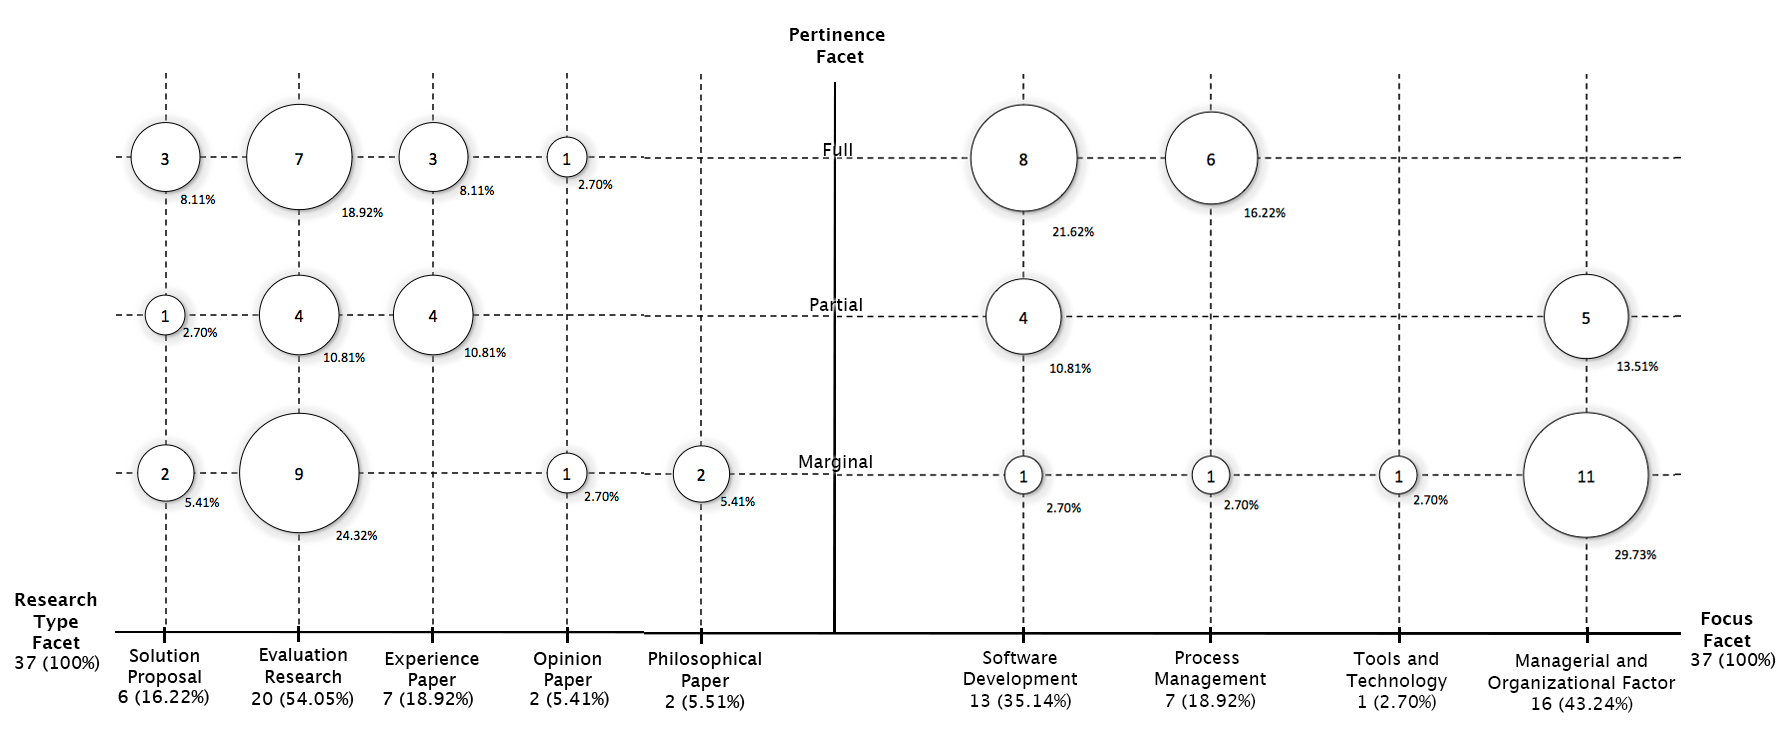
\includegraphics[width=0.8\textwidth,keepaspectratio=true]{figures/PFR.png}
\caption{Systematic map - \textit{Pertinence}, \textit{focus} and \textit{research type}}\label{fig:ms:pfr}
\end{figure}
%%end figure

\twocolumn

By analyzing  in depth the three bubble charts representing the  \textit{systematic map} of the selected studies, we report a list of most significant observations:


\begin{itemize}

\item First of all, by looking at the \textit{pertinence} facet we can observe that only 14 papers (37.84\%)  are entirely dedicated to software development in startups, and 9 of those produced a \textit{weak contribution} (\textit{advice and implications (5)}; \textit{lesson learned (3)}; \textit{tool} (1)).
\item  Observing the \textit{focus} facet, it is easy to see how 16 articles (43.24\%) are focused on \textit{Managerial and organizational factors}, which are only relatively interesting under a SE perspective. In fact, none of those 16 articles have a \textit{full pertinence}.
\item The overall \textit{contribution types} produced by the studies are for the greater part \textit{weak} (24 items, 64.86\%). Of the 13 remaining studies (35.13\%), which produces a \textit{strong contribution type}, only 4 have the \textit{focus} on what is considered fundamental for our research problem (\textit{software development} and \textit{process management}).
\item A good portion of the selected studies were carried out using an \textit{evaluation research} (20 items, 54.05\%)  which is the only \textit{research type} which involves a field study. However, by simultaneously looking at other facets, we can observe how 11 of these evaluation researches are related to \textit{managerial and organizational factors} , and only 7 out of 20 have a \textit{full pertinence} with engineering activities in software startups. On the other hand the \textit{contribution types}, produced by  \textit{evaluation researches}, are widely distributed on the map, whilst other - less empirical - \textit{research types} generally brought only to \textit{weak contribution types}.
\item 14 out of 20 studies, with \textit{focus} on \textit{process management} (7) and \textit{software development} (13), have a \textit{full pertinence} with our research area.
\end{itemize}


So, if we don't consider items which produced a \textit{poor contribution type}, items which do not have \textit{full pertinence} with software development in startups and items with a non-empirical research approach, only four studies remain (\cite{Coleman2008,Coleman2008a,Coleman2007,Kajko-Mattsson2008}), and represent the most prominent contribution to the field.

% subsection publication_distribution (end)

\subsection{Contextual features of startups} % (fold)
\label{sub:contextual_features_of_startups}
In this part we present the results of the data extraction process described in Subsection \ref{sect:rm:ms:extraction}, where we identified peculiar characteristics of startup companies as described in the literature. The results confirms that there is no agreement on a standard definition which specify what exactly a startup is. Different authors provide different definitions and they use the term \textit{startup} referring to context which are often quite different. This makes any attempt to identify a solid and coherent body of knowledge very challenging.

Defining what makes a software startup unique is an interesting problem: apparently is not strictly related to the size of the company. For instance, some authors call \textit{“startups”}, companies with 6 employees \cite{Mirel2000}, whilst others refer to \textit{startups} with more than 300 employees \cite{Yoffie1999,Coleman2008}. It is not about the age of the company either : some authors studied \textit{startups} which have been operating for many years \cite{Lai2010}, while others are more strict about companies recently founded \cite{Kajko-Mattsson2008}. For other authors \textit{start-up} is a phase, and it is not clear where to draw the line anyway. Others claim that startups works on \textit{innovative} products, but they don’t give  the exact definition of innovation, which makes this factor a little confusing (a recent systematic study identified  \textit{``41 definitions of innovation in 204 selected primary SE studies''} \cite{Ali2010a}).

To illustrate how authors use the term \textit{software startup}, we systematically extracted \textit{themes} which characterize companies inquired in the selected relevant studies. We were able to identify 15 main \textit{themes} which are reported in Table \ref{tab:ms:themes}. The last two columns on the right side indicate respectively the frequency of occurrence of a specific theme and its references.

\onecolumn
\scriptsize
 \begin{longtable}{|p{0.2in}|p{1in}|p{2.3in}|p{0.47in}|p{0.82in}|}
   \hline \hline
 ID & Theme & Description & Frequency  & Ref. \\
    \hline
    
    \endfirsthead
	\multicolumn{5}{c}
	{\tablename\ \thetable\ -- \textit{Continued from previous page}} \\
   		\hline \hline
     		 ID & Theme & Description & Frequency  & Ref. \\
		\hline
\endhead
\hline
\multicolumn{5}{c}
{\tablename\ \thetable\ -- \textit{Continued on next page}} \\
\endfoot
\endlastfoot

T.1 & Lack of resources & Economical, human, and physical resources are extremely limited. & 13 & \cite{Yogendra2002}, \cite{Yoffie1999}, \cite{Crowne2002}, \cite{Kajko-Mattsson2008}, \cite{Camel1994a}, \cite{Coleman2008a}, \cite{Coleman2007}, \cite{Coleman2008}, \cite{Hanna2010}, \cite{Sutton2000}, \cite{Ambler2002}, \cite{Stanfill2007}, \cite{Tanabian2005} \\
T.2 & New company & The company has been recently created. & 4 & \cite{Crowne2002}, \cite{Yoffie1999}, \cite{Camel1994a}, \cite{Chorev2006} \\
T.3 & Small Team & Startups  starts with a small numbers of individuals. & 7 & \cite{Zettel2001}, \cite{Yoffie1999}, \cite{Crowne2002}, \cite{Kajko-Mattsson2008}, \cite{Sutton2000}, \cite{Chorev2006}, \cite{Tanabian2005} \\
T.4 & Uncertainty & Startups deal with a highly uncertain ecosystem under different perspectives: market,product features, competition, people and finance & 8 & \cite{Heitlager2007}, \cite{Kim2005}, \cite{Coleman2008a}, \cite{Coleman2007}, \cite{Coleman2008}, \cite{Fayad1997}, \cite{Midler2008}, \cite{Tanabian2005}, \cite{Hilmola2003} \\
T.5 & Little working history & The basis of an organizational culture are not present initially. & 2 & \cite{Yoffie1999}, \cite{Ambler2002} \\
T.6 & Higly Risky & Failure rate of startups is extremely high. & 4 & \cite{Heitlager2007}, \cite{Kajko-Mattsson2008}, \cite{Camel1994a}, \cite{Tanabian2005} \\
T.7 & Not self-sustained & Especially in the early stage startups need external funding to sustain their activities (Venture Capitalisst, Angel Investments, Personal Funds, ...) & 2 & \cite{Zettel2001}, \cite{Hanna2010} \\
T.8 & Low-experienced team & A good part of the development team is formed by people with less than 5 years of experience and often recently graduated students. & 5 & \cite{Camel1994a}, \cite{Coleman2008a}, \cite{Coleman2007}, \cite{Ambler2002}, \cite{Kakati2003} \\
T.9 & Flat organization & Startups are usually founders-centric and everyone in the company has big responsabilities. No high-management. & 4 & \cite{Yoffie1999}, \cite{Kajko-Mattsson2008}, \cite{Silva2005}, \cite{Tanabian2005} \\
T.10 & One product & Company's activities gravitate around one product/service only. & 7 & \cite{Ambler2002}, \cite{Kuvinka2011}, \cite{Bean2005}, \cite{Deias}, \cite{Silva2005}, \cite{Coleman2008}, \cite{Taipale2010} \\
T.11 & Innovation & Given the highly competitive ecosystem, startups need to focus on highly innovative segments of the market. & 11 & \cite{Heitlager2007}, \cite{Yogendra2002}, \cite{Mirel2000}, \cite{Steenhuis2008}, \cite{Jansen2008}, \cite{Lai2010}, \cite{Sutton2000}, \cite{Hasel2010}, \cite{Hasel2010}, \cite{Midler2008}, \cite{Kakati2003} \\
T.12 & Time-pressure & The environment often forces startups to  release fast and to work under constant pressure ( terms sheets, demo days, investors' requests ) & 8 & \cite{Zettel2001}, \cite{Camel1994a}, \cite{Coleman2008}, \cite{Tingling2007}, \cite{Sutton2000}, \cite{Deakins2005}, \cite{Hilmola2003}, \cite{Mater2000} \\
T.13 & Highly Reactive & Startups are able to quickly react to changes of the underlying  market, technologies, and product. (compared to more established companies ) & 11 & \cite{Zettel2001}, \cite{Kajko-Mattsson2008}, \cite{Camel1994a}, \cite{Coleman2008a}, \cite{Coleman2008}, \cite{Tingling2007}, \cite{Sutton2000}, \cite{Fayad1997}, \cite{Ambler2002}, \cite{Kuvinka2011}, \cite{Deias}, \cite{Silva2005} \\
T.14 & Third party dependency & Due to lack of resources,to build their product startups heavily rely on external solutions: External APIs,Open Source Software, outsourcing, COTS, ... & 7 & \cite{Yoffie1999}, \cite{Wood2005}, \cite{Wall2001}, \cite{Jansen2008}, \cite{Lai2010}, \cite{Hanna2010}, \cite{Sutton2000}, \cite{Ambler2002} \\
T.15 & Rapidly Evolving & Successful startups aim to grow and scale rapidly. & 8 & \cite{Yogendra2002}, \cite{Yoffie1999}, \cite{Camel1994a}, \cite{Coleman2008}, \cite{Su-Chan2007}, \cite{Sutton2000}, \cite{Ambler2002}, \cite{Kuvinka2011}, \cite{Deakins2005} 
\\

\hline 
 \hline
\caption{Mapping Study - Recurrent themes }\label{tab:ms:themes}\\
\end{longtable}
\small
\twocolumn

When discussing software startups, thirteen authors reported a general lack of human, physical and economical resources (T.1). For this reason, startups deeply depend upon external software solutions such as third party APIs, COTS and OSS (T.14). Other studies refer to  companies which are able to quickly react to changes in the market and technologies (T.13), under remarkably uncertain conditions (T.4). Some authors indicate that these companies are focused on highly innovative segments of the market (T.11), generally working on a single core-product (T.10) under extremely high time-pressure (T.12). Furthermore, eight authors write about startups as fast growing companies (T.15) designed to rapidly scale-up. Other researches mention a very small founding team (T.3), which is often composed by low-experienced people (T.8) with a very flat organization structure (T.9) where the CEO is sometimes a core developer itself. Finally, other studies agree on the highly risky nature of these businesses (T.13) newly created (T.2) and therefore with no or little working history (T.5).

It is important to understand that the above mentioned contextual factors have a relevant impact on software development activities\footnote{To further attest the validity our theoretical model, in Section \ref{sect:theory:validation} we use the above mentioned \textit{themes} to execute a comparative analysis with the theoretical framework we developed with the \textit{grounded theory} case study.}, making them different from established companies \cite{Sutton2000}. And since there is no common agreement on the use of the term \textit{startup} and its implications, it should be an important responsibility of the authors to specify which kind of companies the study actually refers to, in order to avoid misleading and ambiguous results. In the selected studies, most of the authors used the term \textit{startup} without explicitly mentioning what exactly they meant.

For this reason in Chapter \ref{sect:bg} we specified that our case study and consequently the results of the grounded theory regard to \textit{newly created and product-centered companies, in the time-frame that goes from the idea conception to the release of the first product in highly scalable markets} (this formulation was initially shaped around the definitions used in \cite{Blank2012,  Ries2011, Marmer2011}). We finally dedicated a subsection to discuss the generalizability of results to similar domains (see  Section \ref{sect:theory:generalizab}).

% subsection contextual_features_of_startups (end)


\subsection{Rigor and relevance} % (fold)
\label{sub:rigor_and_relevance_results}

Figure \ref{fig:ms:venue}  shows a  \textit{pie chart} representing the distribution of the relevant sample in the three \textit{venue} categories.

 %%startFigure
 \begin{figure}[H]
\centering
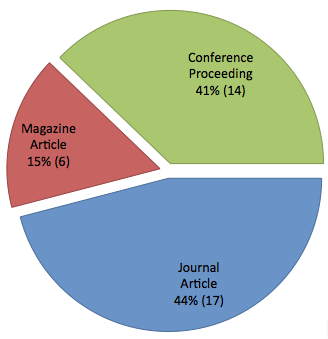
\includegraphics[width=0.3\textwidth,keepaspectratio=true]{figures/venue.png}
\caption{Publication distribution - Venue}\label{fig:ms:venue}
\end{figure}
%%end figure

Despite the scientific validity of a study cannot be a mere consequence of the venue where it has been published, the peer-review process, required for publishing a journal article, is generally much more rigorous and formal than the procedure to get an article published on a scientific magazine or accepted to a conference \cite{ColinRobson2009}. As can be seen in Figure \ref{fig:ms:venue}, only 17 publications (44\%) in the sample are journal articles, while the remaining 56\% consist of conference proceedings and magazine articles. Although this feature alone is not enough to represent a direct implication on the quality\footnote{The publication criteria are determined by the specific editor of the journal/magazine or the committee of a conference. There is a vast multitude of excellent quality studies presented in conference proceedings and magazines, and many example of poor-quality journal articles.}, it can be interpreted as a first indicator of the scientific quality of the sample, formally assessed with the rigor and relevance process here discussed.
	
Following the process described in Subsection \ref{sect:rm:ms:rigor-relevance}, we assessed the \textit{rigor} and \textit{relevance} of each paper by summing up the contribution of individual  \textit{aspects} defined in the evaluation model \cite{Ivarsson2010}. The detailed results of this process are shown in Table \ref{tab:ms:rig-rel-results}. Observe that the maximum possible value for rigor ($Ri=Ri1+Ri2+Ri3$) is 3, and for relevance ($Re=Re1+Re2+Re3$) is 4 (see the detailed quantification Table \ref{tab:ms:quantific-relev-rig}).


\onecolumn
\scriptsize
\begin{longtable}{|l|ccc|c|cccc|c|c|}
\hline \hline
First author (year) & Ri1   & Ri2   & Ri3   & \textbf{Ri} & Re1   & Re2   & Re3   & Re4   & \textbf{Re} & Ref.   \\
\hline 

\endfirsthead
	\multicolumn{11}{c}
	{\tablename\ \thetable\ -- \textit{Continued from previous page}} \\
   		\hline \hline
     		First author (year) & Ri1   & Ri2   & Ri3   & \textbf{Ri} & Re1   & Re2   & Re3   & Re4   & \textbf{Re} & Ref.   \\
		\hline
\endhead
\hline
\multicolumn{11}{c}
{\tablename\ \thetable\ -- \textit{Continued on next page}} \\
\endfoot
\endlastfoot

Coleman (2007) & 1.0   & 1.0   & 1.0   & \textbf{3.0} & 1.0   & 1.0   & 1.0   & 1.0   & \textbf{4.0} & \cite{Coleman2007} \\
Coleman (2008) & 1.0   & 1.0   & 1.0   & \textbf{3.0} & 1.0   & 1.0   & 1.0   & 1.0   & \textbf{4.0} & \cite{Coleman2008a} \\
Coleman (2008) & 1.0   & 1.0   & 1.0   & \textbf{3.0} & 1.0   & 1.0   & 1.0   & 1.0   & \textbf{4.0} & \cite{Coleman2008} \\
Camel (1994) & 0.5   & 1.0   & 1.0   & \textbf{2.5} & 1.0   & 1.0   & 1.0   & 1.0   & \textbf{4.0} & \cite{Camel1994a} \\
H\"{a}sel  (2010) & 0.0   & 1.0   & 1.0   & \textbf{2.0} & 1.0   & 1.0   & 1.0   & 1.0   & \textbf{4.0} & \cite{Hasel2010} \\
Hanna (2010) & 0.0   & 1.0   & 1.0   & \textbf{2.0} & 1.0   & 1.0   & 1.0   & 1.0   & \textbf{4.0} & \cite{Hanna2010} \\
Deakins(2005) & 1.0   & 0.5   & 1.0   & \textbf{2.5} & 1.0   & 1.0   & 0.0   & 1.0   & \textbf{3.0} & \cite{Deakins2005} \\
Chorev (2006) & 1.0   & 1.0   & 0.0   & \textbf{2.0} & 1.0   & 1.0   & 0.0   & 1.0   & \textbf{3.0} & \cite{Chorev2006} \\
Kajko (2008) & 1.0   & 0.5   & 0.0   & \textbf{1.5} & 1.0   & 1.0   & 0.0   & 1.0   & \textbf{3.0} & \cite{Kajko-Mattsson2008} \\
Jansen (2008) & 0.5   & 0.0   & 0.5   & \textbf{1.0} & 1.0   & 1.0   & 0.0   & 1.0   & \textbf{3.0} & \cite{Jansen2008} \\
Midler (2008) & 0.5   & 0.5   & 0.0   & \textbf{1.0} & 1.0   & 1.0   & 0.0   & 1.0   & \textbf{3.0} & \cite{Midler2008} \\
Steenhuis (2008) & 0.0   & 1.0   & 0.0   & \textbf{1.0} & 1.0   & 1.0   & 0.0   & 1.0   & \textbf{3.0} & \cite{Steenhuis2008} \\
Yogendra (2002) & 1.0   & 0.0   & 0.0   & \textbf{1.0} & 1.0   & 1.0   & 0.0   & 1.0   & \textbf{3.0} & \cite{Yogendra2002} \\
Wood (2005) & 0.0   & 0.5   & 0.0   & \textbf{0.5} & 1.0   & 1.0   & 0.0   & 1.0   & \textbf{3.0} & \cite{Wood2005} \\
Tingling (2007) & 0.0   & 0.5   & 0.0   & \textbf{0.5} & 1.0   & 1.0   & 0.0   & 1.0   & \textbf{3.0} & \cite{Tingling2007} \\
Su-Chuang (2007) & 0.0   & 0.0   & 0.0   & \textbf{0.0} & 1.0   & 1.0   & 0.0   & 1.0   & \textbf{3.0} & \cite{Su-Chan2007} \\
Sutton (2000) & 1.0   & 0.0   & 0.0   & \textbf{1.0} & 1.0   & 1.0   & 0.0   & 0.0   & \textbf{2.0} & \cite{Sutton2000} \\
Kakati (2003) & 0.0   & 1.0   & 0.0   & \textbf{1.0} & 0.0   & 1.0   & 1.0   & 0.0   & \textbf{2.0} & \cite{Kakati2003} \\
Mater (2000) & 0.5   & 0.0   & 0.0   & \textbf{0.5} & 1.0   & 1.0   & 0.0   & 0.0   & \textbf{2.0} & \cite{Mater2000} \\
Yoffie (1999) & 0.5   & 0.0   & 0.0   & \textbf{0.5} & 1.0   & 1.0   & 0.0   & 0.0   & \textbf{2.0} & \cite{Yoffie1999} \\
Deias  (2002) & 0.5   & 0.0   & 0.0   & \textbf{0.5} & 1.0   & 1.0   & 0.0   & 0.0   & \textbf{2.0} & \cite{Deias} \\
Silva (2005) & 0.0   & 0.0   & 0.0   & \textbf{0.0} & 1.0   & 1.0   & 0.0   & 0.0   & \textbf{2.0} & \cite{Silva2005} \\
Wall (2001) & 0.0   & 0.0   & 0.0   & \textbf{0.0} & 1.0   & 1.0   & 0.0   & 0.0   & \textbf{2.0} & \cite{Wall2001} \\
Kuvinka (2011) & 0.0   & 0.0   & 0.0   & \textbf{0.0} & 1.0   & 1.0   & 0.0   & 0.0   & \textbf{2.0} & \cite{Kuvinka2011} \\
Mirel (2000) & 0.0   & 0.0   & 0.0   & \textbf{0.0} & 1.0   & 1.0   & 0.0   & 0.0   & \textbf{2.0} & \cite{Mirel2000} \\
Zettel (2001) & 0.5   & 0.0   & 0.5   & \textbf{1.0} & 1.0   & 0.0   & 0.0   & 0.0   & \textbf{1.0} & \cite{Zettel2001} \\
Ambler (2002) & 0.0   & 0.0   & 0.0   & \textbf{0.0} & 1.0   & 1.0   & 0.0   & 0.0   & \textbf{2.0} & \cite{Ambler2002} \\
Stanfill (2007) & 0.5   & 0.5   & 0.0   & \textbf{1.0} & 0.0   & 1.0   & 0.0   & 0.0   & \textbf{1.0} & \cite{Stanfill2007} \\
Taipale (2010) & 0.0   & 0.0   & 0.0   & \textbf{0.0} & 1.0   & 1.0   & 0.0   & 0.0   & \textbf{2.0} & \cite{Taipale2010} \\
Sau-ling Lai (2010) & 0.0   & 0.0   & 0.0   & \textbf{0.0} & 1.0   & 1.0   & 0.0   & 0.0   & \textbf{2.0} & \cite{Lai2010} \\
Kim (2005) & 0.5   & 0.0   & 1.0   & \textbf{1.5} & 0.0   & 0.0   & 0.0   & 0.0   & \textbf{0.0} & \cite{Kim2005} \\
Crowne (2002) & 1.0   & 0.0   & 0.0   & \textbf{1.0} & 0.0   & 0.0   & 0.0   & 0.0   & \textbf{0.0} & \cite{Crowne2002} \\
Heitlager (2007) & 1.0   & 0.0   & 0.0   & \textbf{1.0} & 0.0   & 0.0   & 0.0   & 0.0   & \textbf{0.0} & \cite{Heitlager2007} \\
Himola (2003) & 0.5   & 0.0   & 0.0   & \textbf{0.5} & 0.0   & 0.0   & 0.0   & 0.0   & \textbf{0.0} & \cite{Hilmola2003} \\
Bean (2005) & 0.0   & 0.0   & 0.0   & \textbf{0.0} & 0.0   & 0.0   & 0.0   & 0.0   & \textbf{0.0} & \cite{Bean2005} \\
Fayad (1997) & 0.0   & 0.0   & 0.0   & \textbf{0.0} & 0.0   & 0.0   & 0.0   & 0.0   & \textbf{0.0} & \cite{Fayad1997} \\
Tanabian (2005) & 0.0   & 0.0   & 0.0   & \textbf{0.0} & 0.0   & 0.0   & 0.0   & 0.0   & \textbf{0.0} & \cite{Tanabian2005} \\

\hline \hline
\caption{Mapping Study - Rigor-relevance results }\label{tab:ms:rig-rel-results}\\
 \end{longtable}

\small
\twocolumn


The table is sorted by placing at the top the studies, which received the highest scores in the two dimensions summed together. It is straightforward to observe that Coleman’s studies received the maximum score for both scientific rigor and industrial relevance. By contrast, there are many papers which report a $0$ score (11 zeros for rigor, 7 zeros for relevance), providing a first confirmation of what was only a suspect about the generally low reliability of a good part of these studies.

To further extract useful insight, it is more convenient to adopt a graphical representation of the rigor and relevance. We use the same approach previously utilized to depict the \textit{systematic map} : a bubble chart where the bubble size is proportional to the number of publications, corresponding to the coordinates \textit{x-y}, along with some statistical data shown for each dimension (Figure \ref{fig:ms:rigor-rel-map}).

 %%startFigure
\begin{figure}[H]
\centering
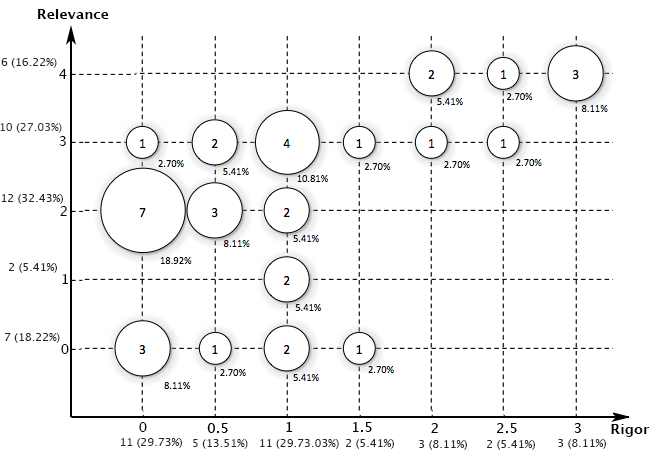
\includegraphics[width=0.50\textwidth,keepaspectratio=true]{figures/rigor-relevance-map.png}
\caption{Rigor-relevance overview}\label{fig:ms:rigor-rel-map}
\end{figure}
%%end figure


If we don’t consider studies in the highest region of scores (see the top-right part of Figure \ref{fig:ms:rigor-rel-map}) for industrial \textit{rigor} ($\geq 2$) and \textit{relevance} ($\geq 3$) from the rest, it is easy to observe how the greater part of the selected studies (78.38\%) received mediocre scientific rigor and industrial relevance scores. Only 8 items belong to the \textit{high-score region}.

% subsection rigor_and_relevance (end)

\section{Analysis of the state-of-the-art} %-------- ## ----------------- ## ----------------- ## ----------------- ## ----------------- ## ---------
 \label{sect:discussion}
This section discus xyz and is organized as following

\subsection{Topics treated in the literature}

Beside the obvious high-frequency of the keyword \textit{software-startup}, a pronounced interest for topics such as \textit{management}  (19 times), \textit{software-process} (17),  \textit{agile-methodologies} (10)  and \textit{web-development} (7) is visible. For software-process, it is worth noticing how studies are concentrated around \textit{process-improvement} (4) and \textit{process-formation} (2).  Among the different agile methodologies, a particular consideration is given to \textit{extreme programming} (7), while other methodologies such as \textit{RUP} (2) and \textit{Scrum} (1) received little attention. This represents a first evidence of our initial assumptions that, in the general meaning of the word, startups are \textit{agile} companies.

Among others, we can observe some topics that are quite peculiar for this area, such as \textit{time-to-market} (6), \textit{rapid-development} (3) and \textit{founder} background (14).

The particular attention given by the literature to those topics, especially aspects related to the   \textit{team},  \textit{agile-methodologies}, \textit{time-to-market},  and  \textit{web-development}, helped us in refining the specific research domain, contributing to adjust the trajectory  of the \textit{case study} conducted with startups' practitioners (see Section \ref{sect:rm:gt}) and driving the formation of a \textit{theoretical model}, which is presented and explained in Section \ref{sect:theory:high-level}. However, the wide variety of topics, combined with the very-low frequency in which each topic appears, represents a symptom of a general scarcity of primary studies investigating specific issues.

\subsection{Systematic map and distribution}

More than 80\% of the studies in the selected sample have been published in the last ten years, which compared to the long-standing history of the SE discipline and more in general software companies (half of a century), is a quite short time-frame. Only 7 relevant articles dated prior to 2002 discuss software startup related issues\footnote{Other 4 articles were discarded in the selection process because they didn’t comply with the selection criteria and then considered as obsolete (see screening process in Subsection \ref{sect:rm:ms:screening}).}. To make a comparison, when looking at one of the closest domain such as software engineering in small companies, we can observe how the specific literature started many years before 2002. For example, in 1994 Brodman was already discussing how to adapt the CMM methodology to small organizations \cite{Brodman1994}. Only 10 years later we find an empirical study inquiring startups and development methodologies \cite{Silva2005}.

The yearly distribution of publications attest the novelty of the startup phenomenon, which has been basically enabled and amplified by the potentially huge markets and distribution channels offered by the internet and mobile devices \cite{Christensen1997,Kakati2003}. This context posed a set of new problems and challenges which can hardly be faced using traditional approaches \cite{Sutton2000}.


Summarizing the implications regarding the RQ-1.1 (\textit{How is the body of knowledge distributed in literature?}) we have found that:


\begin{itemize}

\item The literature lacks of relevant primary studies which investigate engineering activities in software startups. The 37 selected studies are researches spread across different scientific areas and journals. In addition, they are weakly interrelated by mutual references. This confirms what was partially revealed by the first non-systematic literature survey and, at the same time, discloses a complex underlying field.
\item About 80\% of the studies have been published in the last decade, opening a set of new issues brought by the advent of internet and mobile devices which enabled fast and wide proliferation of software startups. The state-of-the-art under a SE perspective is quite recent,  especially when compared to siblings areas such as SE in small companies, which is much more advanced in terms of number of primary studies and provided evidences.
\item The selected studies focus on a wide variety of topics of which we provided a complete overview. Despite more attention is given to some sort of lightweight methodologies for startups and some discussion about process formation and improvement, the evidence produced are definitely undersized to support the dimension of the actual startup phenomenon.
\item To asses the detailed distribution of the body of knowledge we mapped the identified studies into a classification schema which considers four dimensions, namely: research type, contribution type, main focus and pertinence. Of a total of 37 selected studies, 16 of them (43.24\%) are focused on \textit{managerial and organizational factors}, which are only partially interesting under a SE perspective. Additionally, only 14 studies (37.84\%)  are entirely dedicated to software development in startups and 9 of those produced weak contribution types.
\item Overall, we identified only 4 important contributions to the field that are published in scientific journals, are entirely dedicated to engineering activities in startups, provide strong contribution type and are conducted through an evidence-based research approach \cite{Coleman2008,Coleman2008a,Coleman2007,Kajko-Mattsson2008}. Three of these studies are from the same author, Gerry Coleman.
\end{itemize}


\subsection{Rigor and Relevance}

Moreover, the biggest bubble in the chart shows 7 studies (almost 19\% of the total) which received an average score for industrial relevance ($2$) but only a $0$ for the scientific rigor. This kind of studies, according to the authors of the rigor-relevance model \cite{Ivarsson2010}, presents a major issue: although their findings appear to be somewhat appealing for practitioners (average relevance), the extremely poor scientific rigor of the study will make a possible knowledge transfer to the industry highly unlikely or highly dangerous. Indeed Kitchenham states that one of the most important factors for having academic results applied in the industry is by providing proper scientific evidences of the implications \cite{Kitchenham2005,Kitchenham2004}.

Finally, by looking at how bubbles are distributed on the chart (see Figure \ref{fig:ms:rigor-rel-map}) with no need of sophisticated statistical methods, it is clear the relation between items which received the highest scores for \textit{rigor} and the ones which received the highest score for \textit{relevance}. Since the two dimensions represent two independent variables the result is not straightforward. In this particular sample, it indicates that results of studies, which have been rigorously reported, are generally more relevant for the industry (and vice-versa). By thoroughly analyzing the studies in the high rigor-relevance region, we observed that the authors have strong academic backgrounds but at the same time they have worked for many years in direct contact with startups. This is even more visible when comparing them to the other authors in the sample with lower value of rigor and relevance\footnote{Since it is not possible to obtain a complete background study of each author, we based our assumption on a small biographic review.}. This could somehow explain the reason why, in our sample, the rigorous studies are also highly relevant.

Summarizing the implications regarding the RQ-1.2 (\textit{What is the industrial relevance and scientific rigor of the published studies?}) we have found that:


\begin{itemize}

\item Only 17 publications (44\%) in the sample are journal articles. The remaining 56\% consists of conference proceedings and magazine articles, which usually require a less rigorous peer-review process than a scientific journal publication.
\item By assessing the rigor and relevance of the selected studies with a systematic procedure we attested that the majority of works are poorly relevant for startups and are presented with low scientific rigor. By looking at the detailed rigor-relevance chart, it can be observed how most of the studies are located in the lower region of the rigor-relevance map. Additionally, eleven articles received 0 for scientific rigor, and seven articles received 0 for rigor.
\item Coleman’s studies \cite{Coleman2008,Coleman2008a,Coleman2007}, which appears to be a prominent researcher in this area, received also the highest score both for scientific rigor and industrial relevance. This provided to our research a solid starting point. In fact, these references are used a considerable amount of times throughout the thesis document.
\item Seven studies, which received an average score for industrial relevance, were marked with $0$ for the scientific rigor. Thus, although their results could be potentially relevant ($2$) for the industry, the low rigor makes a possible adoption in startups  highly-risky or highly-unlikely. These studies represent almost 19\% of the total.
\item The most rigorous studies in our sample are highly relevant for practitioners, and vice-versa. We observed that in those cases, the authors are academics with a deep connections with the industry or direct experiences in startups.
\end{itemize}

% subsection state_of_the_art (end)

\subsection{Defining startups} % (fold)
\label{sub:defining_startups}

Summarizing the implications regarding the RQ-1.3 (\textit{What are the features which characterize the context of software development in startups, reported in literature?}) we have found that:

\begin{itemize}

\item Different authors use the word \textit{startup} actually referring to different kind of companies. It is very hard to identify an explicit definition of the context in which the companies operate, often given for granted. Under these conditions, trying to identify a coherent body of knowledge is even more challenging and is even harder for practitioners to somewhat adopt the results without having a proper context. For instance, some results about \textit{``startups''} have been obtained by studying companies with  more than 200 employees and others from companies with 6 employees. To make an example, from a SE engineering point of view, the size of the company actually have several implications on the software development activities \cite{Wangenheim2006}.

\item To capture the implicit contextual features that authors used when referring to software startup companies we identified a set of 15 main \textit{themes} and counted their frequency in the selected studies. The most frequent reported themes concern the general lack of resources, highly reactiveness and flexibility, intense time-pressure, uncertain conditions and fast growth.
\item Since the contextual boundaries of startups resulted to be highly blurred, it is responsibility of the researchers who refer to \textit{``startups''} to explicitly mention which are the features of the company that the study is actually concerned with (in most of selected studies an explicit contextualization has been neglected). For this reason we explicitly declared the area of interest of our case study in Introduction (see Chapter \ref{sect:intro}).
\end{itemize}



\subsection{Summary of findings} % (fold)
\label{sub:summary_of_findings}


In this subsection we provide the overall answer to the RQ-1 : \textit{What is the current state-of-the-art in the SE literature pertaining to engineering activities in startups?}.

To emphasize the importance of articles, which brought prominent contributions to the area under investigation, we followed the procedure described in Subsection \ref{sect:rm:ms:ranking}, computing  a score (in the range $[0-10]$) for each selected study.  Table \ref{tab:ms:score-weights} lists the dimensions which were used to assign the final score,  next to the arbitrary weight to balance the ranking criteria.
% subsection summary_of_findings (end)


\begin{table}[H]
\renewcommand{\arraystretch}{1.3}
\caption{Ranking weights }
\label{tab:ms:score-weights}
\centering
\scriptsize \begin{tabular}{|l|l|l|}
\hline 
\hline 
$W$ & Dimension (id) & Weight \\
\hline 
$w_1$ & Pertinence (P) & .25 \\
$w_2$ &Rigor (Ri) & .175 \\
$w_3$ &Relevance (Re) & .175 \\
$w_4$ &Age (A)   & .15 \\
$w_5$ &Venue (V) & .1 \\
$w_6$ &Contribution (C) & .05 \\
$w_7$ &Research type (R) & .05 \\
$w_8$ &Focus (F) & .05 \\
\hline 
\hline 
&\textbf{TOTAL:} & \textbf{1} \\

 \hline  \hline
 \end{tabular}
 \end{table}
%endtable

The most important dimension, counting for the 25\% alone, is \textit{Pertinence}, followed by \textit{rigor} and \textit{relevance}, respectively counting 17.5\% each.  The remaining dimensions are increasingly less important to the final score, which is computed for each paper $i$ by adding up the contributions as shown in the formula below.

\scriptsize  $Score_i = (w_1\cdot P_i) + (w_2 \cdot Ri_i) + (w_3 \cdot Re_i) + (w_4 \cdot A_i) + (w_5 \cdot V_i) + (w_6 \cdot C_i)+ (w_7 \cdot R_i) + (w_8 \cdot F_i)  $
\small 


The final score is presented in Table \ref{tab:ms:rig-rel-rank}. The dimensions, which contributed to the final score, are the columns representing: (A)ge, (Ri)gor, (Re)levance, (V)enue, (P)ertinence, (C)ontribution type, (R)esearch type and (F)ocus. 
\onecolumn
\scriptsize
\begin{longtable}{|l|c|c|c|c|c|c|c|c|c|c|}
\hline \hline
First author (year) & \textbf{Score} & A   & Ri & Re & V & P & C & R  & F & Ref. \\
\hline 
\endfirsthead
	\multicolumn{11}{c}
	{\tablename\ \thetable\ -- \textit{Continued from previous page}} \\
   		\hline \hline
     		 First author (year) & \textbf{Score} & A   & Ri & Re & V & P & C & R  & F & Ref. \\
		\hline
\endhead
\hline
\multicolumn{11}{c}
{\tablename\ \thetable\ -- \textit{Continued on next page}} \\
\endfoot
\endlastfoot

Coleman (2008) & \textbf{9.70} & 1.20  & 1.75  & 1.75  & 1.00  & 2.50  & 0.50  & 0.50  & 0.50  & \cite{Coleman2008} \\
Coleman (2007) & \textbf{9.70} & 1.20  & 1.75  & 1.75  & 1.00  & 2.50  & 0.50  & 0.50  & 0.50  & \cite{Coleman2007} \\
Coleman (2008) & \textbf{9.70} & 1.20  & 1.75  & 1.75  & 1.00  & 2.50  & 0.50  & 0.50  & 0.50  & \cite{Coleman2008a} \\
Kajko (2008) & \textbf{8.09} & 1.20  & 0.88  & 1.31  & 0.70  & 2.50  & 0.50  & 0.50  & 0.50  & \cite{Kajko-Mattsson2008} \\
H\"{a}sel  (2010) & \textbf{7.47} & 1.50  & 1.17  & 1.75  & 1.00  & 0.75  & 0.50  & 0.50  & 0.30  & \cite{Hasel2010} \\
Hanna (2010) & \textbf{7.47} & 1.50  & 1.17  & 1.75  & 1.00  & 0.75  & 0.50  & 0.50  & 0.30  & \cite{Hanna2010} \\
Deakins(2005) & \textbf{6.87} & 0.90  & 1.46  & 1.31  & 1.00  & 1.25  & 0.50  & 0.15  & 0.30  & \cite{Deakins2005} \\
Camel (1994) & \textbf{6.61} & 0.15  & 1.46  & 1.75  & 0.70  & 1.25  & 0.30  & 0.50  & 0.50  & \cite{Camel1994a} \\
Silva (2005) & \textbf{6.58} & 0.90  & 0.00  & 0.88  & 1.00  & 2.50  & 0.30  & 0.50  & 0.50  & \cite{Silva2005} \\
Midler (2008) & \textbf{6.55} & 1.20  & 0.58  & 1.31  & 1.00  & 1.25  & 0.40  & 0.50  & 0.30  & \cite{Midler2008} \\
Taipale (2010) & \textbf{6.53} & 1.50  & 0.00  & 0.88  & 0.70  & 2.50  & 0.30  & 0.15  & 0.50  & \cite{Taipale2010} \\
Chorev (2006) & \textbf{6.43} & 0.90  & 1.17  & 1.31  & 1.00  & 0.75  & 0.50  & 0.50  & 0.30  & \cite{Chorev2006} \\
Zettel (2001) & \textbf{6.32} & 0.60  & 0.58  & 0.44  & 1.00  & 2.50  & 0.40  & 0.30  & 0.50  & \cite{Zettel2001} \\
Jansen (2008) & \textbf{6.25} & 1.20  & 0.58  & 1.31  & 0.60  & 1.25  & 0.30  & 0.50  & 0.50  & \cite{Jansen2008} \\
Sutton (2000) & \textbf{6.11} & 0.60  & 0.58  & 0.88  & 0.60  & 2.50  & 0.30  & 0.15  & 0.50  & \cite{Sutton2000} \\
Heitlager (2007) & \textbf{6.08} & 1.20  & 0.58  & 0.00  & 0.70  & 2.50  & 0.30  & 0.30  & 0.50  & \cite{Heitlager2007} \\
Tingling (2007) & \textbf{5.99} & 1.20  & 0.29  & 0.00  & 0.70  & 2.50  & 0.30  & 0.50  & 0.50  & \cite{Tingling2007} \\
Deias  (2002) & \textbf{5.92} & 0.60  & 0.29  & 0.88  & 0.70  & 2.50  & 0.30  & 0.15  & 0.50  & \cite{Deias} \\
Stanfill (2007) & \textbf{5.74} & 1.20  & 0.88  & 1.31  & 0.70  & 0.75  & 0.30  & 0.30  & 0.30  & \cite{Stanfill2007} \\
Wood (2005) & \textbf{5.70} & 0.90  & 0.29  & 1.31  & 1.00  & 1.25  & 0.30  & 0.15  & 0.50  & \cite{Wood2005} \\
Steenhuis (2008) & \textbf{5.65} & 1.20  & 0.58  & 1.31  & 0.70  & 0.75  & 0.30  & 0.50  & 0.30  & \cite{Steenhuis2008} \\
Yogendra (2002) & \textbf{5.55} & 0.60  & 0.58  & 1.31  & 0.70  & 1.25  & 0.30  & 0.50  & 0.30  & \cite{Yogendra2002} \\
Ambler (2002) & \textbf{5.53} & 0.60  & 0.00  & 0.88  & 0.60  & 2.50  & 0.30  & 0.15  & 0.50  & \cite{Ambler2002} \\
Crowne (2002) & \textbf{5.48} & 0.60  & 0.58  & 0.00  & 0.70  & 2.50  & 0.30  & 0.30  & 0.50  & \cite{Crowne2002} \\
Mater (2000) & \textbf{5.45} & 0.60  & 0.29  & 1.31  & 0.70  & 1.25  & 0.50  & 0.50  & 0.30  & \cite{Mater2000} \\
Kakati (2003) & \textbf{5.41} & 0.90  & 0.58  & 0.88  & 1.00  & 0.75  & 0.50  & 0.50  & 0.30  & \cite{Kakati2003} \\
Kuvinka (2011) & \textbf{5.28} & 1.50  & 0.00  & 0.88  & 0.70  & 1.25  & 0.30  & 0.15  & 0.50  & \cite{Kuvinka2011} \\
Su-Chuang (2007) & \textbf{5.26} & 1.20  & 0.00  & 1.31  & 0.70  & 0.75  & 0.30  & 0.50  & 0.50  & \cite{Su-Chan2007} \\
Sau-ling Lai (2010) & \textbf{5.23} & 1.50  & 0.00  & 0.88  & 1.00  & 0.75  & 0.30  & 0.50  & 0.30  & \cite{Lai2010} \\
Mirel (2000) & \textbf{4.98} & 0.60  & 0.35  & 0.88  & 1.00  & 1.25  & 0.30  & 0.30  & 0.30  & \cite{Mirel2000} \\
Himola (2003) & \textbf{4.57} & 0.90  & 0.58  & 0.44  & 1.00  & 0.75  & 0.30  & 0.30  & 0.30  & \cite{Hilmola2003} \\
Kim (2005) & \textbf{4.53} & 0.90  & 0.88  & 0.00  & 0.70  & 0.75  & 0.50  & 0.50  & 0.30  & \cite{Kim2005} \\
Wall (2001) & \textbf{4.28} & 0.60  & 0.00  & 0.88  & 0.60  & 1.25  & 0.30  & 0.15  & 0.50  & \cite{Wall2001} \\
Yoffie (1999) & \textbf{4.22} & 0.60  & 0.29  & 0.88  & 0.60  & 0.75  & 0.30  & 0.50  & 0.30  & \cite{Yoffie1999} \\
Bean (2005) & \textbf{3.50} & 0.90  & 0.00  & 0.00  & 1.00  & 0.75  & 0.30  & 0.15  & 0.40  & \cite{Bean2005} \\
Tanabian (2005) & \textbf{3.10} & 0.90  & 0.00  & 0.00  & 0.70  & 0.75  & 0.30  & 0.15  & 0.30  & \cite{Tanabian2005} \\
Fayad (1997) & \textbf{2.45} & 0.15  & 0.00  & 0.00  & 0.60  & 0.75  & 0.30  & 0.15  & 0.50  & \cite{Fayad1997} \\
\hline 


 \hline
\caption{Mapping Study - Ranking of selected studies }\label{tab:ms:rig-rel-rank}\\
 \end{longtable}

\small
\twocolumn


It can be observed that the same 4 papers which occupy the first 4 positions of the above presented \textit{ranking} (\cite{Coleman2008,Coleman2008a,Coleman2007,Kajko-Mattsson2008}), are in the most interesting regions of the \textit{systematic maps} described before, and at the same time are rated as highly rigorous and relevant (Table \ref{tab:ms:rig-rel-rank}). These studies are, in fact, the ones which mostly guided and supported us in the research process. In particular Coleman's studies received the highest scores mainly because  his works are actually focused on software process in startups from a SE perspective, undertaking rigorous and well documented approaches, and producing meaningful outcomes published on relevant journals. However, we observed that the three publications are, in fact, derived from the same study with 21 companies.

Although a little part of the companies inquired in his publications had an extremely limited number of employees involved in software development, the greatest part of them had more than 20 developers/engineers, making its results hard to generalize to actual early-stage startups with 3 or 4 founding members.

The results of the systematic mapping of the literature, fostered our motivation in filling the gap by executing a case study on early-stage startups. Thus, our case study is clearly distinct from what has already been investigated by Coleman. In fact, the companies, which we inquired in the interviews at the time of the first release, employed an average number of about 8 employees, contrary to Colman's companies which employed up to 190 employees.

Moreover, as Coleman himself admits, his results suffer from a limitation which is not present in our study due to the fact that his respondents were covering high-managerial roles (Managers/CTOs/Head of development) which are in practice \textit{``one or more steps removed''} from actual carrying out of the software development \cite{Coleman2007}. Therefore their opinions are strongly biased towards methodologies they are themselves proposing to their teams. By contrast, in the early stage of the studied startups, the totality of our respondents were directly involved within all the activities of software development, giving to us the possibility to actually attest more reliable data\footnote{As remarked by Coleman, interviewing engineers in mature companies can be misleading to understand the higher-level dynamics, as they might not be aware of all process issues. By contrast, in our research, respondents have been wearing multiple hats during the first stages, acting as managers and engineers at the same time.}.

Finally, we summarize what are the results of the overall systematic mapping, conducted through: creation of a classification schema which was used to map the existing literature; a systematic assessment of the rigor and relevance of the selected studies; and finally identifying contextual features which characterize software startups. The overall results of the analysis are summarized as follows (answering RQ-1):


\begin{itemize}

\item The evidences provided by the 37 selected studies are, for the most part, inadequate to understand the underlying phenomenon of software development in startups. To the current date, twelve years after Sutton assessed that startups have been neglected from process studies \cite{Sutton2000}, the gap has been only partially filled.
\item From the provided \textit{systematic map}, it can be observed that only 13 studies out of 37 selected, are entirely dedicated to the study of software development in startups. The remaining articles are only partially or marginally mentioning relevant contributions to the area. Additionally, by visualizing the four dimensions of the systematic map with the technique proposed by Petersen et al. \cite{Petersen2007}, we were able to provide detailed insights by simultaneously analyzing multiple facets of the literature distribution.

\item The creation of a coherent body of knowledge about software startups is restrained by the fact that different authors use the word \textit{startup} in different contexts (above summarized by showing the more cited contextual \textit{themes}). Some authors use the word \textit{startup} for small new companies while others considered startups companies with hundreds of employees. Others refer to innovative companies or operating in uncertain markets, and for others, \textit{startup} is the name of a phase in a software project. Given this lack of consensus and consistency, when investigating software startups, it is responsibility of the researcher to make explicit mention to the particular context affected by the study. In the selected studies an explicit mention was often neglected, affecting the generalizability of results.
\item The results of selected studies are mediocrely relevant for the industry. Furthermore, considering the general lack of high scientific rigor, it will be very unlikely that the findings can have a real impact on startup companies. Since transferring the knowledge to the companies should be one of the most important concern of SE research \cite{Ivarsson2010}, the next generation of studies should provide more relevant and scientifically rigorous evidences. However, in our sample, we identified a small portion of studies with both very high relevance and very high rigor. We observed that the authors of those papers have generally academic background with strong connections or past experiences with startup companies. This might infer that the combination of excellent academics skills (providing rigor) with practical experience in the field (providing relevance) fosters the quality of a startup-related study.
\item We identified only four prominent contributions to the field by ranking the studies according to a defined score, considering different features of the study. Furthermore we realized that three of these studies, conducted from the same author, are based on the same empirical data collected in 21 companies with different profiles.
\item Some of the features, which characterize startups, are common to other SE domains (innovation, market-driven development, small companies, short time-to-market, \ldots). However, the unique combination of elements, which coexists in modern startup companies, poses a new series of issues which need to be addressed with primary studies in the specific domain. A new and consistent body of knowledge should support activities and decisions of the fast growing number of startup companies, through evidence-based research \cite{Kitchenham2005,Wohlin2000}. The need of more studies is attested by the impressing proliferation of (non-peer reviewed) books dedicated to startups, which quickly became best-sellers (see Appendix \ref{a:related:grey} for detailed books review).
\item Finally, all of the above mentioned results fostered our motivation in pursuing research in this field. In particular, we observed that most studies focused on \textit{mature} startups and we couldn't identify any relevant empirical evidences discussingengineering activities in the very early-stage of the startup creation. This factor contributed in driving the direction of our case study towards a cross-sectional analysis in the time frame that goes from the idea conception to the first release of the product.
\end{itemize}

\section{Work Practices in startups}
//this section is about xyw and is organized as follows, according to our classification schema we will analyze how the literature discuss work practices in startups 


\begin{center}
\begin{tabular}{|l|l|}
\hline
\multicolumn{2}{|c|}{\textbf{Work practices}} \\
\hline
Software Development & 90 \\
Managerial/organizational & 59 \\
Process management & 44 \\
Tools and technology & 6 \\
\hline
Sum & 199\\
\hline
\end{tabular}
\end{center}

\subsection{Overview of Software development in Startups} % (fold)
\label{sub:challenges}

In this chapter we present the most relevant studies contributing to the formation of a \textit{body of knowledge} focused on engineering activities in software startups.  The materials reviewed here were mostly collected during the execution of a systematic review of the literature (detailed in Section \ref{sect:rm:ms}).

The word \textit{startup} appeared in the SE literature for the first time in 1994 in an article written by Carmel \cite{Camel1994a} where he studied the \textit{time-to-completion in young package firm}\footnote{The software development challenges of a startup have changed dramatically in the last 20 years.}. He noticed how these companies were particularly innovative and successful, advocating for the need of more research investigating software development practices so as to replicate success and try to transfer it to other technology sectors.

Only a few engineering studies in this specific area have been published in the years that followed (see Chapter \ref{sect:res}). Moreover the studies we identified in the systematic review appear to be highly fragmented and spread across different areas rather than constituting a consistent \textit{body of knowledge}. In fact, we were able to identify only four empirical SE studies published prior to 2012 which are entirely dedicated to the topic of software development approaches in startups, designed executed and presented in a rigorous way\footnote{Moreover the studies under consideration \cite{Coleman2008,Coleman2008a,Coleman2007,Kajko-Mattsson2008} have investigated mainly mature startups, whilst the empirical research we performed is focused on early-stages startups. This issue is further discussed in the analysis of the systematic literature review (see Section \ref{sect:res:ms})}. In the remaining part of this section we provide an overview of the related works that we have identified during our research.

First of all, a research published in 2000 by Sutton \cite{Sutton2000} confirmed a general lack of  studies in this area, claiming that \textit{``software startups represent a segment that has been mostly neglected in process studies''} and it has been further confirmed with the empirical studies of Coleman et al. \cite{Coleman2008,Coleman2008a,Coleman2007} eight years later.

One of the most prolific SE researcher in the area of startups is Gerry Coleman. He started working with irish startup companies and developing a  \textit{``lightweight software process for startups based on agile practices''} \cite{Coleman2004}, which has been presented at a conference in 2004 \cite{Coleman} but apparently the research evolved into a different direction\footnote{Coleman has been personally contacted and he confirmed that the lightweight process in question has not been further adopted neither \textit{``developed into the later research''}}. Indeed, his attention moved from startups to small enterprises \cite{Coleman2005}. In fact, he published an article titled \textit{``Using grounded theory to understand software process improvement''} \cite{Coleman2007}, which includes detailed explanation of the research methodology undertaken for his analysis. His results show different factors that influence and hinder the formation of processes in startups and small companies.

First insights reveal how software startups are product-oriented in the first period of their development phase \cite{Heitlager2007}. Despite good achievements at the beginning, software development and organizational management increase in complexity \cite{1456074,Banker1998} causing  deterioration of performance over time. Briefly, the necessity of establishing initial repeatable and scalable processes cannot be postponed forever\footnote{This has been confirmed by Peter Thiel, co-founder of \textit{Paypal}, \textit{Asana} and other successful businesses, who declared that \textit{``there is no real chance of setting things up correctly such that the rest unfold easily. But you should still get the early stuff as right as possible''\cite{ThielCS183}.} }.

A study of Kajko-Mattsson  \cite{Kajko-Mattsson2008}, which investigated a Swedish software startup, reported a heavy lack of requirements gathering process, minimal project management, lack of control over the change requests, absence of documentation to track the status and progress of the process and defective releases. Accordingly, Ambler et al. report how two startups approaching to an upcoming IPO started to require processes to focus on scalable solutions, in view of the growing company’s size in terms of users and employees \cite{Ambler2002}. In this regard, Crowne, in \cite{Crowne2002}, specifies different stages through which software startups evolve. Starting without any established workflows, startups grow over time, creating and stabilizing processes to eventually improving them only when sufficiently mature.

As studied in \cite{Tingling2007}, the maturity of a company affects the extent to which processes are adopted. The author reports how introducing Extreme Programming (XP) principles \cite{Beck:2004:EPE:1076267} in the development process was challenging because of the need of trained team-members for fully implementing the methodology\footnote{According to XP creator Kent Beck, to be effective XP requires to be carefully applied :  \textit{``If you follow 80 percent of the process, you get just 20 percent of the benefits''} \cite{Beck:2004:EPE:1076267}.}. In fact, \cite{Silva2005} was able to start with all the XP practices in place only after six months of coaching the team, trying to enhance maturity from day-one. Nevertheless, even then, customization of practices were inevitably implemented to adapt the processes to the undertaken startups’ context \cite{Deias}.

But when startups have no time for training and orienting activities, as discussed in \cite{Sutton2000}, their main focus remains on team capabilities instead of prescriptive processes hiring people who can \textit{``hit the ground running''} \cite{Yoffie1999}. Empowering the team and focus on methodological attributes of the processes oriented in prototyping, proof-of-concepts, mock-ups and demos, to test basic functionalities, have been the primary priority in startups as described in \cite{Camel1994a}. Only when they grow, formal methodologies arise, followed by a conduction of quality assurance and long-term planning processes \cite{Yoffie1999}.

As partially discussed above, contributions to flexibility and reactiveness of the development process has been conducted prominently by means of \textit{Lean} \cite{Gautam2008} and \textit{Agile} \cite{Abrahamsson2002} methodologies (also reported in \cite{Taipale2010, Kuvinka2011}), where the extreme uncertain conditions lead startups to learn fast from trials and errors with a strong customer relationship in order to avoid wasting time in building wrong functionalities and prevent rapidly exhaustion of resources \cite{Midler2008, Hilmola2003, Sutton2000}. Customer involvement in software development has also been discussed in  \cite{Yogendra2002} as important factor to encourage an early alignment of business concerns to the technology strategies, because both are salient considerations to be successful \cite{Tingling2007}.

When startups take a development approach that is mainly product-oriented rather than process-oriented, it is essential to have a flexible team, with a workflow that helps them quickly to change direction according to the target market \cite{Sutton2000}. In this regard, many startups have been focused on team productivity, providing more control to the employees instead of providing them rigid guidelines \cite{Tanabian2005, Chorev2006, Kakati2003}.

Then, when startups are mature enough to support software process improvement (SPI), the solutions considered according to the state-of-the-art are oriented towards light-weight processes such as a design of development process based on XP, proposed by Zettel in \cite{Zettel2001}. The process consists of a set of activities and artifacts (in addition to some important roles) defined in order to identify responsibilities and tools to utilize. But, despite the promising benefits reported by Zettel, we were not able to identify any future evaluation in real-world settings.

Another attempt of SPI in startups has been conducted by Deakins et al. introducing a \textit{Helical Model for managing e-commerce development environment} \cite{Deakins2005}. Also in this case, the author prescribed broad guidelines for a rapid high-quality development process, which underwent limited testing only in academic settings.

The first publication mentioning the problem of \textit{one-size-fits-all}, related to the SPI  representations for startups, is described in \cite{Fayad1997}. The author reveals the problem in actuating the same \textit{best-practices} criteria for established companies in 10-person software startups. Thoroughly remarked in \cite{Sutton2000}, Sutton states that problems of SPI in software startups arise because of: the dynamism of the development process, which precludes repeatability; organizational maturity, that cannot be maintained from startups in view of lack of corporate direction; severe lack of resources, both human and technological for process definition, implementation, management, training \ldots; in conclusion, the primary benefits of SPI do not address startups, which instead of promoting product quality, aim to minimize time-to-market.

Additionally, the role of SPI has always been neglected because seen as an obstacle to the development team’s creativity and flexibility as described in \cite{Coleman2008a} and to the need of a quick delivering product process environment. In fact, product quality is left aside in favour of minimal and suitable functionalities to shorten the time-to-market. As reported in two studies of Mater and Mirel \cite{Mater2000, Mirel2000}, quality aspects, mostly taken in consideration in internet startups, are oriented to usability and scalability, even though the market and application type heavily influences the quality-demand \cite{Coleman2008, Kim2005}.

Finally, to maintain the development activities, oriented to limited but suitable functionality, many studies suggest to externalize the complexity of parts of the project to third party solutions by means of outsourcing activities, software reuse and open-source strategies \cite{Hanna2010, Jansen2008, Wall2001, Bean2005}.

In conclusion, since \textit{``all decisions related to product development are trade-off situations''} \cite{Hilmola2003}, generally startups optimize workflows to the dynamic context they are involved into. In fact they typically adopt any development style that might work to support their first needs in what is called the \textit{``Just do it''} school of software startups \cite{Ries2011}. Additionally, as remarked by Coleman, \textit{``many managers just decide to apply what they know, as their experience tells them it is merely common sense''} \cite{Coleman2008}.

To summarize - although a number of studies have been discussed in this section - the existing material appears to be inadequate to deal with the increasing importance of startups’ demands. In fact, as confirmed by the analysis of results of the systematic review (see Section  \ref{sect:res:ms:summary}) this area appears to be, to some extent, immature. Nonetheless, we are recently assisting an impressive proliferation of books (such as \cite{Blank2012, Ries2011, Christensen1997, RobWalling2010}) and pseudo researches \cite{StartupGenome}, which are gaining traction among practitioners. For this reason we have dedicated a subsection of Appendix \ref{a:related:grey} to review the most relevant part of the \textit{grey literature} which affects our research.


% subsection software_development_in_startups_review (end)

\subsection{Process management practices}
\label{sub:analysis-process}

The process management represents all the engineering activities used to manage product development in startups.  A study of Sutton  \cite{Sutton2000} recognized the need of flexibility to accommodate frequent changes in the development environment, and reactiveness to obtain rapid and timely response in applying methodologies.  Moreover, in a startup all the activities are conducted towards the development of the product and not in improving processes mainly because of scarce resources \cite{Heitlager2007}. Coleman in \cite{Coleman2008a} reports that the activities related to process improvement and process assessments are neglected since they represent a waste of time and money for startups \cite{Fayad1997, Coleman2008}.  

Agile methodologies have been considered the most acceptable processes given their certain degree of freedom in quickly changing direction following the business strategy \cite{Taipale2010}. In this context, fast releases with an iterative and incremental approach shorten the lead time from idea conception to production with fast deployment \cite{Taipale2010}. The benefits  of having  weekly releases and frequent build cycles to help addressing the uncertainty of the market has been further reported by Tingling \cite{Tingling2007}, Ambler \cite{Ambler2002} and Silva \cite{Silva2005}.

In order to shorten time to market, prototyping is essential according to \cite{Deakins2005, Camel1994a}. To allow better prototyping activities, evolutionary workflows are needed to implement "soft-coded" solutions in the first phases until the optimal solution is found \cite{Deakins2005, Sutton2000}. 

Coleman in \cite{Coleman2007} reports how XP is the most used development methodology across startup companies because of the recuded process cost and low level of documentation requirements compared to serial and rigorous methodologies. Nevertheless, the same author confirms that to implement practices effectively, they need to be tailored to the specific features that characterize each development context \cite{Coleman2007, Coleman2008}. This concurs with the practices of allocating varying effort for formalizing specifications, design, documentation and testing in tailored development methodologies \cite{Ambler2002, Zettel2001, Camel1994a} that emphasize the importance of minimal process management.

Finally, to explain this orientation towards of flexible and reactive development approach, startups can be characterized by applying the Cynefin framework \cite{Kurtz2003}. Within this framework, startups cross the complex and chaotic domains. Those two domains represent the areas where applying rigorous process management to control development activities is not effective since solutions are not predictive. Instead, flexible and reactive methods, designed to stimulate customer feedback, increase the number of perspectives and solutions available to a decision maker. Nevertheless, it is not by chance that software startups are more disruptive than established and bureaucratic companies. Moving from complex to chaotic spaces, software startups open up new possibilities of creation, generating the condition for innovation. This dynamic is named divergence-convergence, and it is one of the many movements described by the Cynefin framework. 

//Summarizing paragraph  MISSING: - You need here a short paragraph summarizing your analysis. Mind you: the summary is not about what you have done, but what can be learned ("take away" value) from your analysis.


\subsection{Software development practices}




\begin{center}
\begin{tabular}{|l|l|}
\hline
\multicolumn{2}{|c|}{\textbf{Software Development}} \\
\hline
RE & 19 \\
Analysis & 14 \\
Implementation & 5 \\
QA & 21 \\
Deployment & 2 \\
RE and Analysis & 1 \\
\hline
Sum & 62 \\
\hline
\end{tabular}
\end{center}





\label{sub:analysis-software-dev}
\subsubsection{Requirements Engineering}
\subsubsection{Design and Architecture}
\subsubsection{Implementation and maintenance}
\subsubsection{Quality Assurance}
\subsubsection{Other software development practices}



\subsection{Managerial and organizational practices}

\begin{center}
\begin{tabular}{|l|l|}
\hline
\multicolumn{2}{|c|}{\textbf{Documentation}} \\
\hline
SD Documentation & 3 \\
M Documentation & 4 \\
PM Documentation & 1 \\
\hline
Sum & 8\\
\hline
\end{tabular}
\end{center}


\label{sub:analysis-managerial}


\subsection{Other practices}
\label{sub:analysis-other}
//should be about tools and technologies

\section{Conclusions and future work} %-------- ## ----------------- ## ----------------- ## ----------------- ## ----------------- ## ---------
 \label{sect:concl}

 This text should be replaced with the conclusionsThis text should be replaced with the conclusionsThis text should be replaced with the conclusionsThis text should be replaced with the conclusionsThis text should be replaced with the conclusionsThis text should be replaced with the conclusionsThis text should be replaced with the conclusionsThis text should be replaced with the conclusionsThis text should be replaced with the conclusionsThis text should be replaced with the conclusionsThis text should be replaced with the conclusionsThis text should be replaced with the conclusionsThis text should be replaced with the conclusionsThis text should be replaced with the conclusionsThis text should be replaced with the conclusionsThis text should be replaced with the conclusionsThis text should be replaced with the conclusionsThis text should be replaced with the conclusionsThis text should be replaced with the conclusionsThis text should be replaced with the conclusions. 

This text should be replaced with the conclusionsThis text should be replaced with the conclusionsThis text should be replaced with the conclusionsThis text should be replaced with the conclusionsThis text should be replaced with the conclusionsThis text should be replaced with the conclusionsThis text should be replaced with the conclusionsThis text should be replaced with the conclusionsThis text should be replaced with the conclusionsThis text should be replaced with the conclusionsThis text should be replaced with the conclusionsThis text should be replaced with the conclusionsThis text should be replaced with the conclusionsThis text should be replaced with the conclusionsThis text should be replaced with the conclusionsThis text should be replaced with the conclusionsThis text should be replaced with the conclusionsThis text should be replaced with the conclusionsThis text should be replaced with the conclusionsThis text should be replaced with the conclusions. 

This text should be replaced with the conclusionsThis text should be replaced with the conclusionsThis text should be replaced with the conclusionsThis text should be replaced with the conclusionsThis text should be replaced with the conclusionsThis text should be replaced with the conclusionsThis text should be replaced with the conclusionsThis text should be replaced with the conclusionsThis text should be replaced with the conclusionsThis text should be replaced with the conclusionsThis text should be replaced with the conclusionsThis text should be replaced with the conclusionsThis text should be replaced with the conclusionsThis text should be replaced with the conclusionsThis text should be replaced with the conclusionsThis text should be replaced with the conclusionsThis text should be replaced with the conclusionsThis text should be replaced with the conclusionsThis text should be replaced with the conclusionsThis text should be replaced with the conclusions. 

This text should be replaced with the conclusionsThis text should be replaced with the conclusionsThis text should be replaced with the conclusionsThis text should be replaced with the conclusionsThis text should be replaced with the conclusionsThis text should be replaced with the conclusionsThis text should be replaced with the conclusionsThis text should be replaced with the conclusionsThis text should be replaced with the conclusionsThis text should be replaced with the conclusionsThis text should be replaced with the conclusionsThis text should be replaced with the conclusionsThis text should be replaced with the conclusionsThis text should be replaced with the conclusionsThis text should be replaced with the conclusionsThis text should be replaced with the conclusionsThis text should be replaced with the conclusionsThis text should be replaced with the conclusionsThis text should be replaced with the conclusionsThis text should be replaced with the conclusions. 



\appendix
\label{sect:app}

\subsection{Search Strings}
\label{sub:a_search_string}
The search strings, utilized to retrieve relevant studies (see Subsection \ref{sect:rm:ms:conduct}), have been adapted to the underlying search technology, as shown in  Table \ref{tab:ms:search-strings}.


\onecolumn
\scriptsize
\begin{longtable}{|p{5.3in}|}
\hline    \hline 


\multicolumn{1}{|c|}{String A - Compendex/Inspec \cite{compendex}} \\
\hline 

 \endfirsthead

	\multicolumn{1}{c}
	{\tablename\ \thetable\ -- \textit{Continued from previous page}} \\
                \hline
\endhead


\multicolumn{1}{c}
{\tablename\ \thetable\ -- \textit{Continued on next page}} \\
\endfoot
\endlastfoot
\hspace{1in}\\
('early-stage firm' OR 'early-stage company' OR 'high-tech venture' OR 'high-tech ventures' OR 'high-tech start-up' OR 'high-tech start-ups' OR 'high-tech startups' OR 'high-tech startup' OR 'start-up company' OR 'start-up companies' OR 'startup company' OR 'startup companies' OR 'software startup' OR 'lean startup' OR 'lean start-up' OR 'lean startups' OR 'software startups' OR 'software package startups' OR 'software package start-up' OR 'software package start-ups' OR 'software package startup' OR 'IT start-ups' OR 'IT start-up' OR 'IT startup' OR 'IT startups' OR 'software start-up' OR 'software start-ups' OR 'software product startup' OR 'software product startups' OR 'software start up' OR 'web startup' OR 'web start-up' OR 'web startups' OR 'web start-ups' OR'internet startup' OR 'internet start-up' OR 'internet startups' OR 'internet start-ups' OR 'mobile startup' OR 'mobile start-up' OR 'mobile startups' OR 'mobile start-ups')AND (develop* OR engineer* OR model* OR construct* OR implement* OR cod* OR creat* OR build*) AND (software OR product* OR service* OR process* OR methodolog* OR tool* OR method* OR practice* OR artifact* OR artefact*  OR qualit* OR 'non-functional requirement' OR 'non-functional requirements' OR ilit* OR strateg*)  \\
\hspace{3in}\\
\hline \hline 


\multicolumn{1}{|c|}{String B - IEEE xplore \cite{IEEExpl}} \\
\hline  
\hspace{1in}\\
('early-stage firm' OR 'early-stage company' OR 'high-tech venture' OR 'high-tech ventures' OR 'start-up company' OR 'start-up companies' OR 'startup company' OR 'high-tech start-up' OR 'high-tech start-ups' OR 'high-tech startups' OR 'high-tech startup' OR 'startup companies' OR 'software startup' OR 'lean startup' OR 'lean start-up' OR 'lean startups' OR 'software startups' OR 'software package startups' OR 'software package start-up' OR 'software package start-ups' OR 'software package startup' OR 'IT start-ups' OR 'IT start-up' OR 'IT startup' OR 'IT startups' OR 'software start-up' OR 'software start-ups' OR 'software product startup' OR 'software product startups' OR 'software start up' OR 'web startup' OR 'web start-up' OR 'web startups' OR 'web start-ups' OR'internet startup' OR 'internet start-up' OR 'internet startups' OR 'internet start-ups' OR 'mobile startup' OR 'mobile start-up' OR 'mobile startups' OR 'mobile start-ups') AND (development OR developing OR engineer OR engineering OR model OR construct* OR implement* OR cod* OR creat* OR build*) AND (software OR product OR products OR service OR services OR process OR processes OR artifact* OR artefact* OR quality OR qualities OR 'non-functional requirement' OR 'non-functional requirements' OR ilities OR methodology OR methodologies OR tool OR tools OR method OR methods OR practice OR practices OR strategy OR strategies) \\
\hspace{3in}\\
\hline \hline

\multicolumn{1}{|c|}{String C - Scopus \cite{scopus}} \\
\hline
\hspace{1in}\\
ABS(('early-stage firm' OR 'early-stage company' OR 'high-tech venture' OR 'high-tech ventures' OR 'start-up company' OR 'start-up companies' OR 'high-tech start-up' OR 'high-tech start-ups' OR 'high-tech startups' OR 'high-tech startup' OR 'startup company' OR 'startup companies' OR 'software startup' OR 'lean startup' OR 'lean start-up' OR 'lean startups' OR 'software startups' OR 'software package startups' OR 'software package start-up' OR 'software package start-ups' OR 'software package startup' OR 'IT start-ups' OR 'IT start-up' OR 'IT startup' OR 'IT startups' OR 'software start-up' OR 'software start-ups' OR 'software product startup' OR 'software product startups' OR 'software start up' OR 'web startup' OR 'web start-up' OR 'web startups' OR 'web start-ups' OR'internet startup' OR 'internet start-up' OR 'internet startups' OR 'internet start-ups' OR 'mobile startup' OR 'mobile start-up' OR 'mobile startups' OR 'mobile start-ups')AND (develop* OR engineer* OR model* OR construct* OR implement* OR cod* OR creat* OR build*) AND (software OR product* OR service* OR process* OR artifact* OR artefact*  OR qualit* OR 'non-functional requirement' OR 'non-functional requirements' OR ilit* OR methodolog* OR tool* OR method* OR practice* OR strateg*) ) \\
\hspace{3in}\\
\hline  \hline
%%
\pagebreak
%%
\multicolumn{1}{|c|}{String D - ISI Web of Knowledge \cite{ISIweb}} \\
\hline   
\hspace{1in}\\
TS=(('early-stage firm' OR 'early-stage company' OR 'high-tech venture' OR 'high-tech ventures' OR 'start-up company' OR 'start-up companies' OR 'high-tech start-up' OR 'high-tech start-ups' OR 'high-tech startups' OR 'high-tech startup' OR 'startup company' OR 'startup companies' OR 'software startup' OR 'lean startup' OR 'lean start-up' OR 'lean startups' OR 'software startups' OR 'software package startups' OR 'software package start-up' OR 'software package start-ups' OR 'software package startup' OR 'IT start-ups' OR 'IT start-up' OR 'IT startup' OR 'IT startups' OR 'software start-up' OR 'software start-ups' OR 'software product startup' OR 'software product startups' OR 'software start up' OR 'web startup' OR 'web start-up' OR 'web startups' OR 'web start-ups' OR'internet startup' OR 'internet start-up' OR 'internet startups' OR 'internet start-ups' OR 'mobile startup' OR 'mobile start-up' OR 'mobile startups' OR 'mobile start-ups')AND (develop* OR engineer* OR model* OR construct* OR implement* OR cod* OR creat* OR build*) AND (software OR product* OR service* OR process* OR artifact* OR artefact*  OR qualit* OR 'non-functional requirement' OR 'non-functional requirements' OR ilit* OR methodolog* OR tool* OR method* OR practice* OR strateg*))   \\
\hspace{1in}\\
\hline  \hline

\multicolumn{1}{|c|}{String E - ACM \cite{ACMsearch}} \\
\hline 
\hspace{1in}\\
((Abstract:('early-stage firm' OR 'early-stage company' OR 'high-tech venture' OR 'high-tech ventures' OR 'start-up company' OR 'start-up companies' OR 'startup company' OR 'startup companies' OR 'software startup' OR 'lean startup' OR 'lean start-up' OR 'high-tech start-up' OR 'high-tech start-ups' OR 'high-tech startups' OR 'high-tech startup' OR 'lean startups' OR 'software startups' OR 'software package startups' OR 'software package start-up' OR 'software package start-ups' OR 'software package startup' OR 'IT start-ups' OR 'IT start-up' OR 'IT startup' OR 'IT startups' OR 'software start-up' OR 'software start-ups' OR 'software product startup' OR 'software product startups' OR 'software start up' OR 'web startup' OR 'web start-up' OR 'web startups' OR 'web start-ups' OR'internet startup' OR 'internet start-up' OR 'internet startups' OR 'internet start-ups' OR 'mobile startup' OR 'mobile start-up' OR 'mobile startups' OR 'mobile start-ups')) AND (Abstract:(develop* OR engineer* OR model* OR construct* OR implement* OR cod* OR creat* OR build*)) AND (Abstract:('software' OR product* OR service* OR process* OR methodolog* OR tool* OR method* OR practice* OR artifact* OR artefact*  OR qualit* OR 'non-functional requirement' OR 'non-functional requirements' OR ilit* OR strateg*))) \\
\hspace{3in}\\
\hline  \hline

 
\multicolumn{1}{|c|}{String F - Google Scholar \cite{gScholar}} \\
\hline  
\hspace{1in}\\
('software startup' OR 'software startups')AND (develop* OR engineer* OR cod* OR creat* ) AND (software OR product* OR process* OR methodolog* OR tool* OR method* OR practice* OR artifact* OR qualit* OR 'non-functional requirements' OR strateg*)  \\
\hspace{3in}\\
\hline  \hline 
\caption{Search strings}\label{tab:ms:search-strings}\\

 \end{longtable}

\small
\twocolumn


% A: Online contribution ---- ---- ---- ---- ---- ---- ---- ---- ---- ---- ---- ---- ---- ---- 

\subsection{Selected studies overview}
\label{sub:a_one_line}
We extracted a brief  \textit{one-line} sentence which summarize the content of each study and can be used by the reader to grasp the idea behind the articles without reading the full text. A set of keywords have been assigned to each article during the initial stages of creation of the classification schema (see analysis of results in Section \ref{sect:res:ms}). The result of this process is presented in Table \ref{tab:ms:oneline}.

\onecolumn
\scriptsize 
\begin{longtable}{|p{0.2in}|p{0.8in}|p{2.5in}|p{1.4in}|}

    \hline    \hline
    Ref.  & Author (year) &  One-line contribution & Keywords \\
    \hline    
    
     \endfirsthead
	\multicolumn{4}{c}
	{\tablename\ \thetable\ -- \textit{Continued from previous page}} \\
   		\hline \hline
     		  Ref.  & Author (year) &  One-line contribution & Keywords \\
		\hline
\endhead
\hline
\multicolumn{4}{c}
{\tablename\ \thetable\ -- \textit{Continued on next page}} \\
\endfoot
\endlastfoot

\cite{Coleman2008} & Coleman (2008) & ' [...] the previous experience of the person tasked with managing the development work is the prime influencer on the process a company initially uses. Other influencers include the market sector in which the company is operating, the style of management used and the size and scale of the company operations.' & Software Process, Process formation, Resources,  Founder, XP, RUP, Agile Methodologies.  \\ \hline  
\cite{Coleman2007} & Coleman (2007) & 'Background of Software Development Manager was central to the initial process that a software company used.' & Software Process, Software Process Improvement, Grounded Theory, Factors Influencing Process.  \\ \hline 
\cite{Coleman2008a} & Coleman (2008) & 'Our research found that SPI programmes are implemented reactively and many software managers are reluctant to implement SPI best practice models because of the associated costs.' & Software Process, Software Process Improvement, Grounded Theory, Factors Influencing Process.  \\ \hline 
\cite{Kajko-Mattsson2008} & Kajko-Mattsson (2008) & By applying their process in a start-up they obtained good results: manage requirements, define development release, and control releases, improve quality. & Process improvement, Software Process, Release Management, Communication, Maintenance, Founder, early-stage, Improve Quality. \\ \hline 
\cite{Hasel2010} & H\'{a}sel  (2010) & '[...] the competence profiles preferred by founders with innovative products differ from those preferred by founders with less innovative products.' & Founder Background, Founder Teams, IT competence, Team, Know-how. \\ \hline 
\cite{Hanna2010} & Hanna (2010) & The model presented in this paper offers a powerful tool for understanding the challenges of offshoring & Outsourcing, Offshore, Know-how, Management, decision-making. \\ \hline 
\cite{Deakins2005} & Deakins(2005) & 'The dotcom development environment is highly volatile and requirements can change rapidly in response to competitor offerings and customer needs; customers are unreliable predictors of their future needs. Need of multi-skilled teams, adaptiveness over efficiency, rapid development, early-stage, experimentation, improvement based on customer' & Innovation, management, software Process, volatile environment, time-to-market, rapid Development,web-development. \\ \hline 
\cite{Camel1994a} & Camel (1994) & 'The presence of several other time-to-completion accelerators appears to be weak in software startups: they did not fully use development methodologies, they made little for increasing use of software tools to increase productivity, weak risk analysis and project control' & Time-to-market, Package Software, Founder, Software Process, Tools. \\ \hline 
\cite{Silva2005} & Silva (2005) & 'We have successfully used all of XP practices, adopted most of them and even came up with some unique practices of our own.' & XP, Software Process, Agile methodologies, Practices, Adaption, Rapid Changes. \\ \hline 
\cite{Midler2008} & Midler (2008) & 'While exploitation provides vital short-term resources,exploration enhances the adaptation of the organization to a changing environment because it increases the variance of organizational activities' & Management, Multi-project, Software Process, Maturity, Learning, Internet, Founder, Uncertainty. \\ \hline 
\cite{Taipale2010} & Taipale (2010) & 'Our workflow is predictable within acceptable variance and we can change direction of the business at any given time'  & XP, Lean, Agile Methodologies, Software Process, Pivoting. \\ \hline 
\cite{Chorev2006} & Chorev (2006) & 'Marketing is very important for success and is underestimated by product startups [...] core team competences is crucial as well' & Management, Software Process, Influencing Factors, Success, Marketing, early-stage, Team Competences. \\ \hline 
\cite{Zettel2001} & Zettel (2001) & 'This paper proposes a lightweight software process for a specific application domain (i.e., database-and user-interface-oriented off-the-shelf e-business applications).' & Process Improvement, XP, Agile Methodologies, Lightweight process, IT, Project Management. \\ \hline 
\cite{Jansen2008} & Jansen (2008) & 'Here, we describe two start-ups that have opportunistically and pragmatically developed their products, reusing functionality from
others that they could never have built independently.' & Reuse, Product-line, Unstructured, Method, third-party, Founder, IT, COTS. \\ \hline 
\cite{Sutton2000} & Sutton (2000) & 'Startups represent a software industry segment that has been mostly neglected in process studies, and it is possible that lessons drawn from start-ups also apply to other develop-ment organizations.' & Software Process, Process formation,  early-stage,Time-to-market, Resources. \\ \hline 
\cite{Heitlager2007} & Heitlager (2007) & 'These companies start very ad-hoc, trying to overcome the uncertainties of market, team and platform. The biggest struggle for these companies is to survive with only scarce resources.' - This paper provides a matrix to analyze the dynamics of the maturity of product development. & Software Process,  early-stage, Innovation, Internet, Process Improvement, Product Development. \\ \hline 
\cite{Tingling2007} & Tingling (2007) & 'Small releases, on-site customer, continuous integration and refactoring were most vigorously advanced by management and adopted by developers. Paired programming on the other hand was culturally avoided.' & Rapid Development, XP, IT, Software Process, Internet, Practices, Agile methodologies. \\ \hline 
\cite{Deias} & Deias  2002) & 'We are enthusiastic about XP, and it is difficult for us to imagine a software project where we should not try to use XP, at least in the domain of Internet development.' & Software Process, Agile Methodologies, XP, Web Development, Risk Management, Project Management, Internet, Quality Assurance, Business, Founder,Customer relation. \\ \hline 
\cite{Stanfill2007} & Stanfill (2007) & 'To improve the chances of successfully adopting a new technological innovation and boosting entrepreneurial team performance, we propose an improved way to select suitable technologies, better timing for delivering market-driven requirements to product designers, and enhanced understanding of the implications of business and technical decisions with regards to impact on intellectual property.' & Team Performance, Market Feasibility, Management, Market-driven Requirements,  early-stage, Founder,Technology-Driven decisions, IT.\\ \hline 
\cite{Wood2005} & Wood (2005) & 'Taken together, these strategies provide guidance to entrepreneurs, board members and business and engineering managers of startups for the effective use of Open Source Software.' & Open Source, Release, Software development,  early-stage,Strategy, Internet,  Cost-reduction,License. \\ \hline 
\cite{Steenhuis2008} & Steenhuis (2008) & 'It is therefore unlikely that follower regions or nations are able to catch-up with the leading regions or nations unless the leading regions or nations enter the high portion of the S-curve, i.e. their economic growth slows down.' & Innovation, Technological Development, Critical Mass,Business,Economic Growth Internet, Business. \\ \hline 
\cite{Yogendra2002} & Yogendra (2002) & 'With the role of technology varying from 'enabler' to 'driver' of the business strategy, business and technology strategies need be in close alignment' & Management, Technology Driven Decisions, Planning, Monitoring, Quality. \\ \hline 
\cite{Ambler2002} & Ambler (2002) & 'I wondered whether the rules of software development had also changed. Were we witnessing a paradigm shift in the way we develop software?' & Agile Methodologies, Web Development, RUP, Comparison, Paradigm-shift. \\ \hline 
\cite{Crowne2002} & Crowne (2002) & 'A model for the evolution of product development from startup to maturity is provided, consisting of three phases:phases: Startup ,Stabilization , Growth [...] Successful development of new software products is a key value driver for many startup companies.' & Software Process,  Founder, Life-Cycle, Internet, Maturity. \\ \hline 
\cite{Mater2000} & Mater (2000) & 'Short-time-to market, fast growth, changing requirement are Entrepreneurs dream and Engineer nightmare' & Management, Business,Web Development, Quality, UX, Time-to-Market. \\ \hline 
\cite{Kakati2003} & Kakati (2003) & 'Product uniqueness was shown not to be a significant factor in determining initial success, despite the tendency of high-tech firm to emphasize RnD and technological excellence' & Management, Success Criteria, Risk. \\ \hline 
\cite{Kuvinka2011} & Kuvinka (2011) & 'Scrum involves many meetings, much planning overhead, and time-consuming team collaboration. Is it possible for a single writer to keep up?' & Management, Internet, Business, Agile Methodologies, early-stage, Scrum, Kanban. \\ \hline 
\cite{Su-Chan2007} & Su-Chuang (2007) & ' [...] a properly constructed value proposition is essential to the value creation process in e-business, and value is essential to the value creation process in e-business, and value co-production is the building blocks for value protection mechanism in network economy' & Value Proposition, Web Development, E-Business, Internet, Business, Value,Co-production. \\ \hline 
\cite{Lai2010} & Sau-ling Lai (2010) & 'Technology is not Alibaba's core competency (non tech-founder) [...] Customer First, employee next [...] Small is beautiful' & Web Development, Founder Background, Know-how, Value Proposition, Finance, Customer Relation, IT, Internet, Product Design , Business.\\ \hline 
\cite{Mirel2000} & Mirel (2000) & 
' [...] usability improvements depend on more than innovative and user-centered technical designs and implementations. Equally important for creating useful and usable software are the social and political forces that shape the development context.' & Organizational Factors, Usability, Political Support, Sociology, IT, Conflicts, Internet,  Innovation. \\ \hline 
\cite{Hilmola2003} & Himola (2003) & 'On the basis of the results of this article, it is suggested that the improvement of product development lead time is one of the most important parameters in the software startup environment [...] all decisions related to product development are tradeoff situations.' & Time-to-market, Improvement,Business, Management, Finance. \\ \hline 
\cite{Kim2005} & Kim (2005) & 'Initial trust is regarded as a critical factor for many e-businesses to succeed in the business-to-customer e-markets, especially startups, because it creates initial relationships with customers.' & Trust, Customer Relation, Initial Trust,  b2c, E-commerce, Internet, early-stage, Quality. \\ \hline 
\cite{Wall2001} & Wall (2001) & 'When money are scarce, OSS can help your business launch without breaking your budget' & Open Source, Tool, Java, Software development, License, Distributed Development, Cost-reduction. \\ \hline 
\cite{Yoffie1999} & Yoffie (1999) & 'That youthfulness also helps to explain why most start-ups fail: exuberance can only get you so far. Jim Clark and Marc Andreessen made a conscious choice to scale the company with a different type of person. They targeted maturity as well as technical expertise.' & Management, Internet, Web Development, Team Formation. \\ \hline 
\cite{Bean2005} & Bean (2005) & 'Smaller firms like Aperture Technologies Inc. are using wikis to brainstorm, track projects, write and edit documentation, and coordinate marketing. Software startups like Stata Lab-oratories Inc. are using wikis to lower teleconferencing costs for outsourced engineering to India!' & Open Source, Method, Tool, Internet,  Communication, IT, Knowledge Management, Management. \\ \hline 
\cite{Tanabian2005} & Tanabian (2005) & 'Because of the small size of the firm, the amount of uncertainty of its business, and lack of financial strength, Many practices in place may appear to be in contradiction with guidelines for a productive and healthy job.' & Management,  Founder, Job Design, Business, Team Performance, IT, Features, Workload, Internet. \\ \hline 
\cite{Fayad1997} & Fayad (1997) & 'The process should be treated differently from startups to established companies  [...] 'startup effect' in which new initiatives get much more highly qualified and motivated people than standard projects, and the idea of 'heroic efforts' ' & Software Process, IT, Process Improvement, Developers Skill, Resources Scarcity, Internet,  Motivation.  \\ \hline 

\hline 
\hline 

 \caption{ Mapping study - One line content review }\label{tab:ms:oneline}\\
\end{longtable}
\small
\twocolumn



% Ranking quantification
\subsection{Ranking quantification}
\label{sub:a_ranking}


In this appendix we refer to the process of ranking the selected studies as discussed in \textit{Research Methodology}, specifically in Subsection \ref{sect:rm:ms:ranking}. The final score has been computed by summing up contributions from eight dimensions: age; rigor; relevance; venue; pertinence; contribution type; research type; and focus. For each dimension we defined conversion tables to quantify our criteria, i.e. - assigning  higher scores to recent rigorous journal articles entirely devoted to the topic and presenting empirical results relevant to practitioners.

The left table (a) shows the scores assigned to each subcategory of the classification schema, while the table on the right side (b) shows the scores associated to the remaining dimensions.

\begin{figure}[H]
\centering
\subtable[Other dimensions]{ %change
\scriptsize 

 \begin{tabular}{|l|l|}

\hline
\hline 
\multicolumn{2}{|c|}{\textbf{Rigor}} \\ 
\hline 
Ri & Score \\
\hline 
3  & 10 \\
2.5  & 8.33 \\
2 & 6.67 \\
1.5  & 5 \\
1  & 3.33 \\
.5  & 1.67 \\
0  & 0 \\
\hline \hline
\multicolumn{2}{|c|}{\textbf{Relevance}} \\  
\hline
Re & Score \\
\hline 
4     & 10 \\
3     & 7.5 \\
2     & 5. \\
1     & 2.5 \\
0     & 0 \\
\hline \hline
\multicolumn{2}{|c|}{\textbf{Age}} \\

\hline 

Age & Score \\
\hline 
$[0,2]$ & 10 \\
$[3,5]$ & 8 \\
$[6,9]$ & 6 \\
$[10,14]$ & 4 \\
$[15,40]$ & 1 \\
\hline  \hline
\multicolumn{2}{|c|}{\textbf{Venue}} \\

\hline 

Venue & Score \\
\hline 
 Journal Article & 10 \\
Conference Proceeding & 7 \\
Magazine Article & 6 \\



 \hline 
\hline
 \end{tabular}
 
}
\subtable[Classification schema]{
\scriptsize 
 \begin{tabular}{|p{1.35in}|p{0.3in}|}

\hline 
\hline  

\multicolumn{2}{|c|}{\textbf{Research}} \\ 
\hline 
  
Type &	Score\\
\hline  
Evaluation Research & 10 \\ 
Solution Proposal & 6 \\   
Philosophical Papers & 3 \\ 
Opinion Papers & 3 \\ 
Experience Papers & 3 \\

\hline \hline
\multicolumn{2}{|c|}{\textbf{Focus}} \\
\hline  
  Type & Score\\
\hline
Software development & 10 \\ 
Process management & 10 \\ 
Tools and technology & 8 \\ 
Managerial/organizational & 6 \\ 
\hline \hline

\multicolumn{2}{|c|}{\textbf{Pertinence}} \\
\hline  
  Type & Score\\
\hline

Full  & 10 \\ 
Partial & 5 \\ 
Marginal & 3 \\



\hline \hline
\multicolumn{2}{|c|}{\textbf{Contribution}} \\
\hline 
Type &	Score\\
\hline  
Model & 10 \\  
Theory & 10 \\ 
Framework/Methods & 8 \\  
Guidelines & 6 \\  
Lesson learned & 6 \\   
Advice/Implications & 6 \\    
Tool  &  6 \\

 \hline 
\hline
 \end{tabular}


}
\caption[Optional caption for list of figures]{Conversion table for the scoring function}
\label{fig:ms:score-conversion}
\end{figure}
\small

The results of the final ranking of studies is presented in Subsection \ref{sect:res:ms:summary}, while limitations of this approach are discussed in Subsection \ref{sect:rm:ms:validity:sele}.



\subsection{Work practices extraction}
\label{sub:a_tables_work_practices}

\onecolumn

Version one 

\begin{center}
\scriptsize
\begin{longtable}{|p{0.4in}|p{3in}|p{1.3in}|p{1in}|p{0.3in}|}

\hline
References & One-line comment & Work practice & Category & Evidence \\
 & & & & provided \\
\hline
\endfirsthead
\hline
References & One-line comment & Work practice & Category & Evidence \\
 & & & & provided \\
\hline
\endhead
\hline
\multicolumn{5}{c}
{\tablename\ \thetable\ -- \textit{Continued on next page}} \\
\endfoot
\endlastfoot
\cite{Wall2001} & The open source community helped in support product development with no costs & Rely on open source community support & Managerial/organizational & 1 \\
\cite{Taipale2010} & To find subjects for improvements & Measure lead time and cycle time & Managerial/organizational & 0 \\
\cite{Tingling2007} & 40-h workweek (be flexible but regular workdays) & 40-h work week & Managerial/organizational & 1 \\
\cite{Tingling2007} & Code was officially shared but developers exhibited possessiveness & Collective Ownership & Managerial/organizational & 1 \\
\cite{Tingling2007} & Communication simple, formal but ambiguous & System metaphor & Managerial/organizational & 1 \\
\cite{Chorev2006} & High communication between development and marketing team to facilitate spotting product/market fit. & Communication marketing-engineering; & Managerial/organizational & 2 \\
\cite{Ambler2002} & Collective ownerships under SVN of the architectural docs & Collective Ownership of architecture & Managerial/organizational & 2 \\
\cite{Zettel2001} & Documentation specialist writes an online help and user guide book & Create user doc & Managerial/organizational & 2 \\
\cite{Zettel2001} & Documentation is not viable in the short term but essential for the long run & Documentation & Managerial/organizational & 2 \\
\cite{Mater2000} & Costumer in the internet are not tollerant, and competitve solutions are just one click away & Plan for robustness & Managerial/organizational & 1 \\
\cite{Kajko-Mattsson2008} & Plan to release the product & Release deployment & Managerial/organizational & 2 \\
\cite{Kajko-Mattsson2008} & Assignation of tasks to developers & Release development & Managerial/organizational & 2 \\
\cite{Kajko-Mattsson2008} & Start with the release scope preparation defining functionalities to include. Delay has been decreased & Release management process & Managerial/organizational & 2 \\
\cite{Kajko-Mattsson2008} & prioritization of requirements, release cycle has been improved by planning & Release planning & Managerial/organizational & 2 \\
\cite{Ambler2002} & Chef-architect makes models visible to every developers and collect feed-backs & Visibility of the architectures & Managerial/organizational & 2 \\
\cite{Zettel2001} & Everyone collect metrics (testing, progress, velocity, quality) & Collect metrics & Managerial/organizational & 2 \\
\cite{Ambler2002} & Because of growth & Hiring new developers & Managerial/organizational & 2 \\
\cite{Zettel2001} & Project manager bases his decisions (effort estimations, schedules and priorities) on collected metrics & Project manager takes decisions for PM & Managerial/organizational & 2 \\
\cite{Stanfill2007} & Engineering students developed a technology in parallel with the market team, and frequently independently. This was an issue that limited the project. & Separate development from market concerns & Managerial/organizational & 1 \\
\cite{Hilmola2003} & Lead time as the main driver for product development & Time-to-market as driver for the development & Managerial/organizational & 2 \\
\cite{Tanabian2005} & Early stage startups demand initial more working hours, more stress and responsabilities in comparison to established companies. & Working over time & Managerial/organizational & 0 \\
\cite{Coleman2007} & Necessity of skipping documentation, lead to excess of tacit knowledge & Documentation & Managerial/organizational & 2 \\
\cite{Coleman2007} & The size of the company influences the attitude towards documentation: the smaller the company the greater the hostility towards documentation & Documentation & Managerial/organizational & 2 \\
\cite{Coleman2008a} & Necessity of skipping documentation, lead to excess of tacit knowledge & Documentation & Managerial/organizational & 2 \\
\cite{Camel1994a} & little project management & No project management & Managerial/organizational & 1 \\
\cite{Camel1994a} & No use of traditional project planning and poorly planned development &       & Managerial/organizational & 1 \\
\cite{Sutton2000} & Empower team improve quality of product, adaptability of process,efficiency and coordination. & Empower team; & Managerial/organizational & 1 \\
\cite{Crowne2002} & focus on single product, create a new version if need customizations. & Focus on single-product & Managerial/organizational & 1 \\
\cite{Crowne2002} & Plan objectives short-medium term & Plan objectives & Managerial/organizational & 1 \\
\cite{Yogendra2002} & Monitor the process continuously to verify the alignment with the business strategy & Monitor process; & Managerial/organizational & 1 \\
\cite{Steenhuis2008} & Select the right skills in people & Skill team; & Managerial/organizational & 0 \\
\cite{Chorev2006} & Core Team expertise, diversified knowledge and harmony are essential for success. Many angels and VCs highlighted the assessment of the core team in investment decision making. Very often start-ups are founded by young people who themselves lack management skills and experience but do not hire suitable managers. This creates difficulties in both R\&D and in the marketing processes. At certain stages, where the start-up lacks expertise, consultants can be useful. & Team skills vital to success & Managerial/organizational & 2 \\
\cite{Coleman2007} & Co-locate the development team to reduce the costs increasing the sharing of the tacit knowledge & Co-locate the development team & Managerial/organizational & 2 \\
\cite{Ambler2002} & Modelling and documentation were separated efforts. & Dedicated people to docs and modelling & Managerial/organizational & 2 \\
\cite{Ambler2002} & Sharing knowledge and collaboration & Developers and testers were close & Managerial/organizational & 2 \\
\cite{Ambler2002} & When scalability problems arise & Hire chief-architect & Managerial/organizational & 2 \\
\cite{Yoffie1999} & Hire developers with self starter personalities with past experience in similar domain & Need of experience in similar domain and self starter personalities & Managerial/organizational & 2 \\
\cite{Yoffie1999} & Youthness of the founders contribute to failure rates. Startups need to hire technical and expertise & Need of expertise & Managerial/organizational & 2 \\
\cite{Tanabian2005} &       & No separation between designers and developers & Managerial/organizational & 0 \\
\cite{Hasel2010} & The competence of founders working with innovative products are different with non innovative & Prefer IT experts in the founding team & Managerial/organizational & 2 \\
\cite{Tanabian2005} & People can and encouraged to work at home but with more control. Due to the large amount of work. & Work from home with flexible hours. & Managerial/organizational & 0 \\
\cite{Midler2008} & Team capability should be able to absorb and learn from trial and error quickly to avoid prolonged time & Learn quickly from trial and error & Managerial/organizational & 1 \\
\cite{Coleman2008} & Empower  team to Enhance creativity and flexibility & Empower team & Managerial/organizational & 2 \\
\cite{Coleman2008a} & Empower  team to Enhance creativity and flexibility & Empower team & Managerial/organizational & 2 \\
\cite{Sutton2000} & Skilled team, because developer should be able to adapt to new roles and face new challenges everyday & Skilled team; & Managerial/organizational & 1 \\
\cite{Camel1994a} & Importance of the core team: highly motivated, homogeneous, history of working together, small, loose organizational structure & Get the right team & Managerial/organizational & 1 \\
\cite{Camel1994a} & working extra hours & Work overtime & Managerial/organizational & 1 \\
\cite{Chorev2006} & Characteristic of the entrepreneur plays a primary role in maximising the scarce resources & Entrepreneur skills primary; & Managerial/organizational & 2 \\
\cite{Kakati2003} & Characteristic of the entrepreneur (Courage , enthusiasm, commitment, leadership) are more important than other technical factor for the success of a startup & Entrepreneur skills primary; & Managerial/organizational & 2 \\
\cite{Coleman2008} & Hire expertise with agile background to improve chances of success & Agile background & Managerial/organizational & 2 \\
\cite{Crowne2002} & Developers are inexperienced and they need to familiarize with software engineering practices to deal with multi-role full-stack challenges & Familiarize with all SE practices & Managerial/organizational & 1 \\
\cite{Coleman2007} & Hire expertise to supply lack of knowledge in critical moments & Hiring expertise & Managerial/organizational & 2 \\
\cite{Coleman2008a} & Hire expertise to supply lack of knowledge in critical moments & Hiring expertise & Managerial/organizational & 2 \\
\cite{Crowne2002} & Promote developers showing both leadership and technical capacity & Endorse leadership AND technical capacity & Managerial/organizational & 1 \\
\cite{Yoffie1999} & Makes specifications free available to everybody & Use of open standard & Managerial/organizational & 2 \\
\cite{Deias} & high experience developers hard to buy-in XP practices & //  // // & Managerial/organizational & 1 \\
\cite{Silva2005} & The work week was not fully respected & 40h work week & Managerial/organizational & 1 \\
\cite{Silva2005} & Senior developers were more comfortable with this practice & Collective code ownership & Managerial/organizational & 1 \\
\cite{Silva2005} & To solve conflicts among developers or with customers & Dirty laundry meeting & Managerial/organizational & 1 \\
\cite{Silva2005} &       & Retrospectives & Managerial/organizational & 1 \\
\cite{Taipale2010} & The Agile process is predictable with acceptable variance, and change direction of the business of any given time & Agile & Process management & 0 \\
\cite{Taipale2010} & The lead time from idea to production is 8 days. Deployment every day & Fast release with continous deployment & Process management & 0 \\
\cite{Coleman2008} & Startups should tailor agile processes and practices since the cost of SPI (time and res.) is too high to afford & Agile process tailoring & Process management & 2 \\
\cite{Coleman2008a} & Startups should tailor agile processes and practices since the cost of SPI (time and res.) is too high to afford & Agile process tailoring & Process management & 2 \\
\cite{Tingling2007} & weekly delivered,  frequent build cycles & Small releases & Process management & 1 \\
\cite{Deias} & Trying to tailor XP harms the effectiveness & (try) to fully follow XP & Process management & 1 \\
\cite{Kajko-Mattsson2008} & Poor documentation ( no process documentation)  led to poor control over the change request, that are postponed to next releases & Documentation & Process management & 2 \\
\cite{Deakins2005} & Just-in-time delivery practices, prototyping & Release fast & Process management & 0 \\
\cite{Kuvinka2011} &       & Definition of done & Process management & 0 \\
\cite{Zettel2001} &       & Plan iterations based on scenarios & Process management & 2 \\
\cite{Camel1994a} & Mock-up, prototypes, demo to customers in order to test functionalities & Prototype & Process management & 1 \\
\cite{Taipale2010} &       & Definition of done & Process management & 0 \\
\cite{Ambler2002} & 6 to 12 weeks & Incremental release in short cycle & Process management & 2 \\
\cite{Taipale2010} & Product queue for listing the features, from 1 to 5 & Kanban product queue & Process management & 0 \\
\cite{Kuvinka2011} &       & Kanban wall & Process management & 0 \\
\cite{Ambler2002} & Tailoring rup to meet specific necessity & RUP   & Process management & 2 \\
\cite{Kuvinka2011} & 2 weeks & Sprint base approach & Process management & 0 \\
\cite{Taipale2010} & Maintain the buffer small enough & The number of features up to seven & Process management & 0 \\
\cite{Kuvinka2011} &       & WIP metric, 3 tasks at the time & Process management & 0 \\
\cite{Ambler2002} & 6 to 12 weeks & Highly iterative process & Process management & 2 \\
\cite{Fayad1997} & Process assessment is considered wasteful & Process assessment & Process management & 0 \\
\cite{Zettel2001} & Viewed as obsolete and irrelevant & Process improvement & Process management & 2 \\
\cite{Coleman2007} & Tailor process to startups' context & Process tailoring & Process management & 2 \\
\cite{Coleman2008} & Tailor process to startups' context & Process tailoring & Process management & 2 \\
\cite{Coleman2007} & XP is the most used across organizations because of the least process cost and low level of documentation requirements & Use XP & Process management & 2 \\
\cite{Zettel2001} & Tailoring of XP but pair programming but with documenting practices & XP practices & Process management & 2 \\
\cite{Sutton2000} & Process definition only high level: leave details at low level to the team. & High-level work-flow; & Process management & 1 \\
\cite{Coleman2008a} & Minimum processes might work & Minimum process & Process management & 2 \\
\cite{Deakins2005} & Evolutionary prototyping with improvements & Prototyping & Process management & 1 \\
\cite{Deakins2005} & Rapid development processes & Rapid development; & Process management & 1 \\
\cite{Sutton2000} & Evolutionary work-flows at high level to allow prototype; & Evolutionary work-flows; & Process management & 1 \\
\cite{Crowne2002} & Start introducing repeatable processes when grow starts to parallelism & Introduce repeatable process in growth & Process management & 1 \\
\cite{Kuvinka2011} & The company was applying scrumban. Scrumban proved to be a great organizational and motivational tool, but working well only if every one is doing it. Scrum emphises the customers and their needs. & Scrumban & Process management & 0 \\
\cite{Camel1994a} & Little effort allocated formalizing specifications, design, documentation and testing & Minimal engineering activities & Process management & 1 \\
\cite{Heitlager2007} & Start with a product centric approach (ad-hoc) to avoid uncertainty of team market and platform, but at certain point the company should be ready to implement some process and scale & From product to process-centric approach; & Process management & 1 \\
\cite{Heitlager2007} & A process is necessary to scale the company activities, and the startup should monitor the state of evolution of process vs. product to be able to take decision on when to introduce some process & Measure process maturity; & Process management & 1 \\
\cite{Camel1994a} & Engineering;marketing in parallel & Overlapping phases & Process management & 1 \\
\cite{Crowne2002} & Begin SPI when market shares and customers are established (mature) & Begin SPI after market stabilized & Process management & 1 \\
\cite{Kakati2003} & After building a first functioning prototype the team should focus on marketing instead of technical. & Prototype and market first; & Process management & 2 \\
\cite{Silva2005} &       & Full XP; & Process management & 1 \\
\cite{Silva2005} & One release every two weeks with one week of bug fixing & Small-release & Process management & 1 \\
\cite{Silva2005} & used XP help trying to reduce time-to-market & XP practices & Process management & 1 \\
\cite{Silva2005} & Even trying to implement XP, developers were more like cowboy coders. & Cow-boy coding; & Process management & 1 \\
\cite{Deakins2005} & Solutions should remain "soft-coded" in the first phases until the optimal solution is found & Prototyping & Process management & 1 \\
\cite{Taipale2010} &       & Code refactoring & Software development & 0 \\
\cite{Taipale2010} &       & Document new features if applicable, especially for interaction with third party & Software development & 0 \\
\cite{Taipale2010} &       & Integration test with CI & Software development & 0 \\
\cite{Taipale2010} &       & Peer-review critical paths & Software development & 0 \\
\cite{Taipale2010} & Helps find actionable issues & Root cause analysis & Software development & 0 \\
\cite{Taipale2010} &       & Simple design & Software development & 0 \\
\cite{Taipale2010} & Those that are related to users. & Trace metrics of product usage & Software development & 0 \\
\cite{Tingling2007} & Coding standards initially avoided  but later implemented & Coding standards & Software development & 1 \\
\cite{Tingling2007} & Code was rarely broken and was continuously compiled & Continuous integration & Software development & 1 \\
\cite{Tingling2007} & Testing was continuous but without advanced scripts & Continuous testing & Software development & 1 \\
\cite{Tingling2007} & CEO and analytic director acted as customers & On-site customer & Software development & 1 \\
\cite{Tingling2007} & Programming were independent most of the time & Pair-Programming & Software development & 1 \\
\cite{Deias} & Actively push developers during planning game to participate & Planning game & Software development & 1 \\
\cite{Tingling2007} & Value engineering balanced features against time and budget & Planning game & Software development & 1 \\
\cite{Tingling2007} & Modules were constantly improved, periodic burst and dramatic improvement occurred. & Refactoring & Software development & 1 \\
\cite{Tingling2007} & Working softer was favoured & Simple design & Software development & 1 \\
\cite{Crowne2002} & Stay close to customers during product development & Proximity to customer & Software development & 1 \\
\cite{Kuvinka2011} &       & Documentation is approached at the end of the user stories, often at the end of the sprint. & Software development & 0 \\
\cite{Camel1994a} & Software architecture not tangible ( lack of documentation of modeling) & Documentation & Software development & 1 \\
\cite{Deakins2005} & Generate alternatives solutions and evaluate them & Analysis & Software development & 1 \\
\cite{Deias} & Developing an architecture is difficult & Lack of architecture & Software development & 1 \\
\cite{Crowne2002} & Startups should capture new requirements, prioritize them, capture feasibility and value! & Requirement Engineering; & Software development & 1 \\
\cite{Kajko-Mattsson2008} &       & Acceptance testing & Software development & 2 \\
\cite{Zettel2001} & Customers use scenarios to judge whether the systems needs anticipated tests & Acceptance tests & Software development & 2 \\
\cite{Zettel2001} & Viewed as obsolete and irrelevant & Code metrics & Software development & 2 \\
\cite{Jansen2008} & Startups take advantage of existing components saving time-to-market. Extending software functionalities from a third party suppliers & Code reuse & Software development & 2 \\
\cite{Zettel2001} & Customer and developers collect user stories effort is estimated. & Collect scenarios & Software development & 2 \\
\cite{Ambler2002} & Define an infrastructure & Enterprise architectural modelling process & Software development & 2 \\
\cite{Midler2008} & Feedback driven patterns to have an high interaction between internal and external factors. Customer provides key to action & Feedback-driven RE & Software development & 1 \\
\cite{Mater2000} & Looking at the basic requirement process and provide raccomendations where the risk exists and what to be done for mitigating. Assessment of the scalability risk for basic architecture and design is very important for internet startups. & Initial risk assessment & Software development & 0 \\
\cite{Camel1994a} & No evidences of risk analysis conducted & No risk analysis & Software development & 1 \\
\cite{Ambler2002} & Only overview of the architecture. No details & Only high-level architecture. & Software development & 2 \\
\cite{Camel1994a} & Family of products built close together enhancing re-use & Re-use & Software development & 1 \\
\cite{Zettel2001} & Include code for unique test cases and write necessary test files for documentation to improve traceability. & Realize scenarios with TDD & Software development & 2 \\
\cite{Ambler2002} & Because of growth & Redevelopment of the system & Software development & 2 \\
\cite{Ambler2002} & Because of growth & Refactor architecture & Software development & 2 \\
\cite{Zettel2001} & Ensure readability and understandability of the code & Refactor system & Software development & 2 \\
\cite{Zettel2001} &       & Release system & Software development & 2 \\
\cite{Zettel2001} & Developers fix a defect described in an open issue report. Or improve quality & Rework code & Software development & 2 \\
\cite{Jansen2008} & SOA saved time and resources using third party services. But changing a component introduce substantial rework. & SOA using third party services & Software development & 2 \\
\cite{Kajko-Mattsson2008} & Contributed to improve faulty releases. & System testing & Software development & 2 \\
\cite{Camel1994a} & Formulating trade-off at the end of the development process in order to speed-up time to market & Trade-off analysis only in retrospective & Software development & 1 \\
\cite{Camel1994a} & Object orient development orientation for package firms & Object oriented development & Software development & 1 \\
\cite{Deakins2005} & Adjust requirements collecting customer feedback & Customer development & Software development & 1 \\
\cite{Ambler2002} & Benefits in having time of discussing and reflect with co-workers & Architecture conducted in parallel with development & Software development & 2 \\
\cite{Taipale2010} &       & Minimum marketable features (MMF) & Software development & 0 \\
\cite{Yoffie1999} & The system should scale with the company size in harmony, early but not late & Prepare for scalability & Software development & 2 \\
\cite{Mater2000} & Expecially scalability, robustness, speed of changing in technology & Understing key failure conditions & Software development & 1 \\
\cite{Sutton2000} & Developers should maximize the amount of code re-used that they are familiar with & Code re-use; & Software development & 1 \\
\cite{Su-Chan2007} & Co-create value with the customer & Costumer involvment & Software development & 0 \\
\cite{Taipale2010} &       & Customer development & Software development & 0 \\
\cite{Mirel2000} & But it didn't allow a proper feasibility study & Use unpredictability & Software development & 1 \\
\cite{Deakins2005} & high-quality product & Quality product & Software development & 1 \\
\cite{Midler2008} & Postpone technological choices that are restrictive and can limit flexibility & Post-pone limiting decisions; & Software development & 1 \\
\cite{Mater2000} & Quality assurance team are not formed until the product is not ready to be delivered. But at that time the practices are already established and difficult to change. QA is tipically inexperienced, lack of SE training and no business experience. & Elevate the software assurance function to report directly to the CEO & Software development & 1 \\
\cite{Yoffie1999} & User adopters as quality assurance team & Involve users for QA & Software development & 2 \\
\cite{Mater2000} & Increased quality from outsourcing & Outsourcing QA & Software development & 0 \\
\cite{Zettel2001} & Time spent on QA is reduced because of time-to-market pressure & QA    & Software development & 2 \\
\cite{Tanabian2005} & Not clear requirements. The design team must adapt to this frequent and changing & no risk analysis & Software development & 0 \\
\cite{Mater2000} & Introduce a process to understand the costumer quality needs & Costumer feedbacks & Software development & 1 \\
\cite{Mirel2000} & Go to customers to learn their needs. It was a good approach to enhance usability of the product. & Customer involvement & Software development & 1 \\
\cite{Wall2001} & To rank the companies' priorities around the customers' needs & Customer Involvement & Software development & 2 \\
\cite{Su-Chan2007} & Monitor and collect feedbacks & Customers feedback & Software development & 0 \\
\cite{Su-Chan2007} & Define what product or service you are going to provide & Value proposition & Software development & 0 \\
\cite{Su-Chan2007} & Differentiate your product from customers & Value proposition & Software development & 0 \\
\cite{Su-Chan2007} & Indentify costomer target are & Value proposition & Software development & 0 \\
\cite{Taipale2010} &       & Prioritization with time boxing. WIP is 2 at the time & Software development & 0 \\
\cite{Zettel2001} & Requirement engineering only practiced in abbreviated session & Requirement Engineering; & Software development & 2 \\
\cite{Ambler2002} & Requirement documents based on marketing requirement produced iteratively & Update requirement document quickly & Software development & 2 \\
\cite{Mirel2000} & When user had request the prioritization was conflicting between designers and developers & Balance conflicts in prioritization between usability and product team & Software development & 1 \\
\cite{Ambler2002} & Fixing architectural issues & Specialists for architecture & Software development & 2 \\
\cite{Deias} & Refactoring was difficult, since developers had no experience & Refactoring & Software development & 1 \\
\cite{Wall2001} & Using standard APIs makes switching to another project is an advantage if switching to another project & Standard APIs & Software development & 1 \\
\cite{Jansen2008} & Use third party but offline components than online third party services & Third party offline components & Software development & 2 \\
\cite{Jansen2008} & Reusing cots reinforce the architectural structure of the product & Use of cots & Software development & 2 \\
\cite{Taipale2010} &       & Automated acceptance test & Software development & 0 \\
\cite{Taipale2010} &       & Unit tests & Software development & 0 \\
\cite{Mirel2000} & Usability test on proxy instead of real users. & Proxy users & Software development & 1 \\
\cite{Mater2000} & To risk management for making decisions. Include test planning process, test case development, documentation of testing and reporting. & Traditional testing for making decisions & Software development & 1 \\
\cite{Mirel2000} & Usability test is important for product/market fit & Usability test most important to achieve product/market fit & Software development & 1 \\
\cite{Silva2005} & 1 customer inside the company writing user stories during stand-up meetings & Customer-on site & Software development & 1 \\
\cite{Silva2005} &       & Manual deploy & Software development & 1 \\
\cite{Silva2005} &       & Pair programming & Software development & 1 \\
\cite{Silva2005} &       & Planning game & Software development & 1 \\
\cite{Silva2005} & Developers didn't see immediate value in refactoring in using abstract concepts & Refactoring & Software development & 1 \\
\cite{Silva2005} &       & Simple design & Software development & 1 \\
\cite{Silva2005} & Was hard to implement, lack of supporting technologies, lack of experience made TDD hard to implement & TDD   & Software development & 1 \\
\cite{Silva2005} & Problems with CI because of low experience with version control system. & Use tools for Continuous Integration & Software development & 1 \\
\cite{Silva2005} &       & Code standards & Software development & 1 \\
\cite{Camel1994a} & QA and testing largely absent to reduce development lead time & Quality Assurance & Software development & 1 \\
\cite{Silva2005} &       & Cutting-edge technologies; & Tools and Technology & 1 \\
\cite{Crowne2002} & Choose tools which do not conflict with strategic plan & Right tools & Tools and Technology & 1 \\
\cite{Sutton2000} & Use technology that allows to change quickly & Adopt technologies easy to adapt; & Tools and Technology & 1 \\
\cite{Ambler2002} & Official documentation was HTML base for portability and accessibility & HTML documentation & Tools and Technology & 2 \\
\cite{Wall2001} & Save costs & Open source databases & Tools and Technology & 1 \\
\cite{Wall2001} & Open source ensures more compatibility with other components & Open source technologies & Tools and Technology & 1 \\
\cite{Wood2005} & When a company wants to test the viability of a new technology, requiring a large pool of tester, rapidly evolving academic research, cheaply expand market, faces large number of evaluators and few buyers, Open Source can help overcoming this difficulty & Release Open Source code & Tools and Technologies & 1 \\
\cite{Wood2005} & Use open source COTS  instead of closed source components to have access to the code & Use Open Source components & Tools and Technologies & 1 \\
\cite{Bean2005} & Using online wiki tool for synchronize the docs and accessability is a good practice. It is also easy to implement. & Use of wiki & Tools and Technologies & 1 \\
\cite{Ambler2002} & Support models and diagrams on the whiteboard. Good because requires little training and enforce teamness & Use of whiteboards & Tools and Technologies & 2 \\
\cite{Ambler2002} & When they needed permanent documentation they simply scanned sketch drawings & Use simple tools & Tools and Technologies & 2 \\



\hline
\caption{Work practices}\label{tab:appendix:workpract}\\
\end{longtable}
\end{center}



Version two 




\begin{center}
\scriptsize
\begin{longtable}{|p{0.36in}|p{2.6in}|p{1.2in}|p{0.9in}|p{0.9in}|p{0.2in}|}

\hline
References & One-line comment & Work practice & m &Category & Evidence \\
 & & & & provided \\
\hline
\endfirsthead
\hline
References & One-line comment & Work practice & m & Category & Evidence \\
 & & & & provided \\
\hline
\endhead
\hline
\multicolumn{5}{c}
{\tablename\ \thetable\ -- \textit{Continued on next page}} \\
\endfoot
\endlastfoot
\cite{Taipale2010} & Helps find actionable issues & Root cause analysis & Software development & Analysis & 0 \\
\cite{Deias} & Actively push developers during planning game to participate & Planning game & Software development & Analysis & 1 \\
\cite{Tingling2007} & Value engineering balanced features against time and budget & Planning game & Software development & Analysis & 1 \\
\cite{Deakins2005} & Generate alternatives solutions and evaluate them & Analysis & Software development & Analysis & 1 \\
\cite{Mater2000} & Looking at the basic requirement process and provide raccomendations where the risk exists and what to be done for mitigating. Assessment of the scalability risk for basic architecture and design is very important for internet startups. & Initial risk assessment & Software development & Analysis & 0 \\
\cite{Camel1994a} & No evidences of risk analysis conducted & No risk analysis & Software development & Analysis & 1 \\
\cite{Camel1994a} & Formulating trade-off at the end of the development process in order to speed-up time to market & Trade-off analysis only in retrospective & Software development & Analysis & 1 \\
\cite{Taipale2010} &       & Minimum marketable features (MMF) & Software development & Analysis & 0 \\
\cite{Mater2000} & Expecially scalability, robustness, speed of changing in technology & Understing key failure conditions & Software development & Analysis & 1 \\
\cite{Mirel2000} & But it didn't allow a proper feasibility study & Use unpredictability & Software development & Analysis & 1 \\
\cite{Midler2008} & Postpone technological choices that are restrictive and can limit flexibility & Post-pone limiting decisions; & Software development & Analysis & 1 \\
\cite{Taipale2010} &       & Prioritization with time boxing. WIP is 2 at the time & Software development & Analysis & 0 \\
\cite{Mirel2000} & When user had request the prioritization was conflicting between designers and developers & Balance conflicts in prioritization between usability and product team & Software development & Analysis & 1 \\
\cite{Silva2005} &       & Planning game  & Software development & Analysis & 1 \\
\cite{Zettel2001} &       & Release system & Software development & Deployment & 2 \\
\cite{Silva2005} &       & Manual deploy & Software development & Deployment & 1 \\
\cite{Taipale2010} &       & Simple design & Software development & Design & 0 \\
\cite{Tingling2007} & Working softer was favoured & Simple design & Software development & Design & 1 \\
\cite{Deias} & Developing an architecture is difficult & Lack of architecture & Software development & Design & 1 \\
\cite{Jansen2008} & Startups take advantage of existing components saving time-to-market. Extending software functionalities from a third party suppliers & Code reuse & Software development & Design & 2 \\
\cite{Ambler2002} & Define an infrastructure & Enterprise architectural modelling process & Software development & Design & 2 \\
\cite{Ambler2002} & Only overview of the architecture. No details & Only high-level architecture. & Software development & Design & 2 \\
\cite{Camel1994a} & Family of products built close together enhancing re-use  & Re-use & Software development & Design & 1 \\
\cite{Ambler2002} & Because of growth & Refactor architecture & Software development & Design & 2 \\
\cite{Jansen2008} & SOA saved time and resources using third party services. But changing a component introduce substantial rework. & SOA using third party services & Software development & Design & 2 \\
\cite{Ambler2002} & Benefits in having time of discussing and reflect with co-workers & Architecture conducted in parallel with development & Software development & Design & 2 \\
\cite{Yoffie1999} & The system should scale with the company size in harmony, early but not late & Prepare for scalability & Software development & Design & 2 \\
\cite{Sutton2000} & Developers should maximize the amount of code re-used that they are familiar with & Code re-use; & Software development & Design & 1 \\
\cite{Ambler2002} & Fixing architectural issues & Specialists for architecture & Software development & Design & 2 \\
\cite{Wall2001} & Using standard APIs makes switching to another project is an advantage if switching to another project & Standard APIs & Software development & Design & 1 \\
\cite{Jansen2008} & Use third party but offline components than online third party services & Third party offline components & Software development & Design & 2 \\
\cite{Jansen2008} & Reusing cots reinforce the architectural structure of the product & Use of cots & Software development & Design & 2 \\
\cite{Silva2005} &       & Simple design & Software development & Design & 1 \\
\cite{Tingling2007} & Coding standards initially avoided  but later implemented & Coding standards & Software development & Implemantation & 1 \\
\cite{Tingling2007} & Programming were independent most of the time & Pair-Programming & Software development & Implementation & 1 \\
\cite{Zettel2001} & Viewed as obsolete and irrelevant & Code metrics & Software development & Implementation & 2 \\
\cite{Camel1994a} & Object orient development orientation for package firms & Object oriented development & Software development & Implementation & 1 \\
\cite{Silva2005} &       & Pair programming & Software development & Implementation & 1 \\
\cite{Silva2005} &       & Code standards & Software development & Implementation & 1 \\
\cite{Zettel2001} & Documentation is not viable in the short term but essential for the long run & Documentation & Managerial/organizational & M Documentation & 2 \\
\cite{Coleman2007} & Necessity of skipping documentation, lead to excess of tacit knowledge & Documentation & Managerial/organizational & M Documentation & 2 \\
\cite{Coleman2007} & The size of the company influences the attitude towards documentation: the smaller the company the greater the hostility towards documentation & Documentation & Managerial/organizational & M Documentation & 2 \\
\cite{Coleman2008a} & Necessity of skipping documentation, lead to excess of tacit knowledge & Documentation & Managerial/organizational & M Documentation & 2 \\
\cite{Taipale2010} &       & Code refactoring & Software development & Maintainance & 0 \\
\cite{Tingling2007} & Modules were constantly improved, periodic burst and dramatic improvement occurred. & Refactoring & Software development & Maintainance & 1 \\
\cite{Ambler2002} & Because of growth & Redevelopment of the system & Software development & Maintainance & 2 \\
\cite{Zettel2001} & Ensure readability and understandability of the code & Refactor system & Software development & Maintainance & 2 \\
\cite{Zettel2001} & Developers fix a defect described in an open issue report. Or improve quality & Rework code & Software development & Maintainance & 2 \\
\cite{Deias} & Refactoring was difficult, since developers had no experience & Refactoring  & Software development & Maintanance & 1 \\
\cite{Silva2005} & Developers didn't see immediate value in refactoring in using abstract concepts & Refactoring & Software development & Maintenance & 1 \\
\cite{Kajko-Mattsson2008} & Poor documentation ( no process documentation)  led to poor control over the change request, that are postponed to next releases & Documentation & Process management & PM Documentation & 2 \\
\cite{Taipale2010} &       & Integration test with CI & Software development & QA    & 0 \\
\cite{Taipale2010} &       & Peer-review critical paths & Software development & QA    & 0 \\
\cite{Tingling2007} & Code was rarely broken and was continuously compiled & Continuous integration & Software development & QA    & 1 \\
\cite{Tingling2007} & Testing was continuous but without advanced scripts & Continuous testing & Software development & QA    & 1 \\
\cite{Kajko-Mattsson2008} &       & Acceptance testing & Software development & QA    & 2 \\
\cite{Zettel2001} & Customers use scenarios to judge whether the systems needs anticipated tests & Acceptance tests & Software development & QA    & 2 \\
\cite{Zettel2001} & Include code for unique test cases and write necessary test files for documentation to improve traceability. & Realize scenarios with TDD & Software development & QA    & 2 \\
\cite{Kajko-Mattsson2008} & Contributed to improve faulty releases. & System testing & Software development & QA    & 2 \\
\cite{Deakins2005} & high-quality product & Quality product & Software development & QA    & 1 \\
\cite{Mater2000} & Quality assurance team are not formed until the product is not ready to be delivered. But at that time the practices are already established and difficult to change. QA is tipically inexperienced, lack of SE training and no business experience. & Elevate the software assurance function to report directly to the CEO & Software development & QA    & 1 \\
\cite{Yoffie1999} & User adopters as quality assurance team & Involve users for QA & Software development & QA    & 2 \\
\cite{Mater2000} & Increased quality from outsourcing & Outsourcing QA & Software development & QA    & 0 \\
\cite{Zettel2001} & Time spent on QA is reduced because of time-to-market pressure & QA    & Software development & QA    & 2 \\
\cite{Taipale2010} &       & Automated acceptance test & Software development & QA    & 0 \\
\cite{Taipale2010} &       & Unit tests & Software development & QA    & 0 \\
\cite{Mirel2000} & Usability test on proxy instead of real users.  & Proxy users & Software development & QA    & 1 \\
\cite{Mater2000} & To risk management for making decisions. Include test planning process, test case development, documentation of testing and reporting. & Traditional testing for making decisions & Software development & QA    & 1 \\
\cite{Mirel2000} & Usability test is important for product/market fit & Usability test most important to achieve product/market fit & Software development & QA    & 1 \\
\cite{Silva2005} & Was hard to implement, lack of supporting technologies, lack of experience made TDD hard to implement & TDD   & Software development & QA    & 1 \\
\cite{Silva2005} & Problems with CI because of low experience with version control system.  & Use tools for Continuous Integration & Software development & QA    & 1 \\
\cite{Camel1994a} & QA and testing largely absent to reduce development lead time & Quality Assurance & Software development & QA    & 1 \\
\cite{Taipale2010} & Those that are related to users. & Trace metrics of product usage & Software development & RE    & 0 \\
\cite{Tingling2007} & CEO and analytic director acted as customers & On-site customer & Software development & RE    & 1 \\
\cite{Crowne2002} & Stay close to customers during product development & Proximity to customer & Software development & RE    & 1 \\
\cite{Crowne2002} & Startups should capture new requirements, prioritize them, capture feasibility and value! & Requirement Engineering; & Software development & RE    & 1 \\
\cite{Midler2008} & Feedback driven patterns to have an high interaction between internal and external factors. Customer provides key to action & Feedback-driven RE & Software development & RE    & 1 \\
\cite{Deakins2005} & Adjust requirements collecting customer feedback & Customer development & Software development & RE    & 1 \\
\cite{Su-Chan2007} & Co-create value with the customer & Costumer involvment & Software development & RE    & 0 \\
\cite{Taipale2010} &       & Customer development & Software development & RE    & 0 \\
\cite{Tanabian2005} & Not clear requirements. The design team must adapt to this frequent and changing & Changing requirements & Software development & RE    & 0 \\
\cite{Mater2000} & Introduce a process to understand the costumer quality needs & Costumer feedbacks & Software development & RE    & 1 \\
\cite{Mirel2000} & Go to customers to learn their needs. It was a good approach to enhance usability of the product. & Customer involvement & Software development & RE    & 1 \\
\cite{Wall2001} & To rank the companies' priorities around the customers' needs & Customer Involvement & Software development & RE    & 2 \\
\cite{Su-Chan2007} & Monitor and collect feedbacks & Customers feedback & Software development & RE    & 0 \\
\cite{Su-Chan2007} & Define what product or service you are going to provide & Value proposition & Software development & RE    & 0 \\
\cite{Su-Chan2007} & Differentiate your product from customers & Value proposition & Software development & RE    & 0 \\
\cite{Su-Chan2007} & Indentify costomer target are & Value proposition & Software development & RE    & 0 \\
\cite{Zettel2001} & Requirement engineering only practiced in abbreviated session & Requirement Engineering; & Software development & RE    & 2 \\
\cite{Ambler2002} & Requirement documents based on marketing requirement produced iteratively & Update requirement document quickly & Software development & RE    & 2 \\
\cite{Silva2005} & 1 customer inside the company writing user stories during stand-up meetings & Customer-on site & Software development & RE    & 1 \\
\cite{Zettel2001} & Customer and developers collect user stories effort is estimated.  & Collect scenarios & Software development & RE and Analysis & 2 \\
\cite{Taipale2010} &       & Document new features if applicable, especially for interaction with third party & Software development & SD Documentation & 0 \\
\cite{Kuvinka2011} &       & Documentation is approached at the end of the user stories, often at the end of the sprint. & Software development & SD Documentation & 0 \\
\cite{Camel1994a} & Software architecture not tangible ( lack of documentation of modeling) & Documentation & Software development & SD Documentation & 1 \\
\cite{Zettel2001} & Documentation specialist writes an online help and user guide book & Create user doc & Managerial/organizational & Usability & 2 \\
\cite{Wall2001} & The open source community helped in support product development with no costs & Rely on open source community support & Managerial/organizational &       & 1 \\
\cite{Taipale2010} & To find subjects for improvements & Measure lead time and cycle time & Managerial/organizational &       & 0 \\
\cite{Tingling2007} & 40-h workweek (be flexible but regular workdays) & 40-h work week & Managerial/organizational &       & 1 \\
\cite{Tingling2007} & Code was officially shared but developers exhibited possessiveness & Collective Ownership & Managerial/organizational &       & 1 \\
\cite{Tingling2007} & Communication simple, formal but ambiguous & System metaphor & Managerial/organizational &       & 1 \\
\cite{Chorev2006} & High communication between development and marketing team to facilitate spotting product/market fit. & Communication marketing-engineering; & Managerial/organizational &       & 2 \\
\cite{Ambler2002} & Collective ownerships under SVN of the architectural docs & Collective Ownership of architecture & Managerial/organizational &       & 2 \\
\cite{Mater2000} & Costumer in the internet are not tollerant, and competitve solutions are just one click away & Plan for robustness & Managerial/organizational &       & 1 \\
\cite{Kajko-Mattsson2008} & Plan to release the product & Release deployment & Managerial/organizational &       & 2 \\
\cite{Kajko-Mattsson2008} & Assignation of tasks to developers & Release development & Managerial/organizational &       & 2 \\
\cite{Kajko-Mattsson2008} & Start with the release scope preparation defining functionalities to include. Delay has been decreased & Release management process & Managerial/organizational &       & 2 \\
\cite{Kajko-Mattsson2008} & prioritization of requirements, release cycle has been improved by planning & Release planning & Managerial/organizational &       & 2 \\
\cite{Ambler2002} & Chef-architect makes models visible to every developers and collect feed-backs & Visibility of the architectures & Managerial/organizational &       & 2 \\
\cite{Zettel2001} & Everyone collect metrics (testing, progress, velocity, quality) & Collect metrics & Managerial/organizational &       & 2 \\
\cite{Ambler2002} & Because of growth & Hiring new developers & Managerial/organizational &       & 2 \\
\cite{Zettel2001} & Project manager bases his decisions (effort estimations, schedules and priorities) on collected metrics & Project manager takes decisions for PM & Managerial/organizational &       & 2 \\
\cite{Stanfill2007} & Engineering students developed a technology in parallel with the market team, and frequently independently. This was an issue that limited the project. & Separate development from market concerns & Managerial/organizational &       & 1 \\
\cite{Hilmola2003} & Lead time as the main driver for product development & Time-to-market as driver for the development & Managerial/organizational &       & 2 \\
\cite{Tanabian2005} & Early stage startups demand initial more working hours, more stress and responsabilities in comparison to established companies. & Working over time & Managerial/organizational &       & 0 \\
\cite{Camel1994a} & little project management & No project management & Managerial/organizational &       & 1 \\
\cite{Camel1994a} & No use of traditional project planning and poorly planned development &       & Managerial/organizational &       & 1 \\
\cite{Sutton2000} & Empower team improve quality of product, adaptability of process,efficiency and coordination. & Empower team; & Managerial/organizational &       & 1 \\
\cite{Crowne2002} & focus on single product, create a new version if need customizations. & Focus on single-product & Managerial/organizational &       & 1 \\
\cite{Crowne2002} & Plan objectives short-medium term & Plan objectives & Managerial/organizational &       & 1 \\
\cite{Yogendra2002} & Monitor the process continuously to verify the alignment with the business strategy & Monitor process; & Managerial/organizational &       & 1 \\
\cite{Steenhuis2008} & Select the right skills in people & Skill team; & Managerial/organizational &       & 0 \\
\cite{Chorev2006} & Core Team expertise, diversified knowledge and harmony are essential for success. Many angels and VCs highlighted the assessment of the core team in investment decision making. Very often start-ups are founded by young people who themselves lack management skills and experience but do not hire suitable managers. This creates difficulties in both R\&D and in the marketing processes. At certain stages, where the start-up lacks expertise, consultants can be useful. & Team skills vital to success & Managerial/organizational &       & 2 \\
\cite{Coleman2007} & Co-locate the development team to reduce the costs increasing the sharing of the tacit knowledge & Co-locate the development team & Managerial/organizational &       & 2 \\
\cite{Ambler2002} & Modelling and documentation were separated efforts. & Dedicated people to docs and modelling & Managerial/organizational &       & 2 \\
\cite{Ambler2002} & Sharing knowledge and collaboration & Developers and testers were close & Managerial/organizational &       & 2 \\
\cite{Ambler2002} & When scalability problems arise & Hire chief-architect & Managerial/organizational &       & 2 \\
\cite{Yoffie1999} & Hire developers with self starter personalities with past experience in similar domain & Need of experience in similar domain and self starter personalities & Managerial/organizational &       & 2 \\
\cite{Yoffie1999} & Youthness of the founders contribute to failure rates. Startups need to hire technical and expertise & Need of expertise & Managerial/organizational &       & 2 \\
\cite{Tanabian2005} &       & No separation between designers and developers & Managerial/organizational &       & 0 \\
\cite{Hasel2010} & The competence of founders working with innovative products are different with non innovative & Prefer IT experts in the founding team & Managerial/organizational &       & 2 \\
\cite{Tanabian2005} & People can and encouraged to work at home but with more control. Due to the large amount of work. & Work from home with flexible hours. & Managerial/organizational &       & 0 \\
\cite{Midler2008} & Team capability should be able to absorb and learn from trial and error quickly to avoid prolonged time & Learn quickly from trial and error & Managerial/organizational &       & 1 \\
\cite{Coleman2008} & Empower  team to Enhance creativity and flexibility & Empower team & Managerial/organizational &       & 2 \\
\cite{Coleman2008a} & Empower  team to Enhance creativity and flexibility & Empower team & Managerial/organizational &       & 2 \\
\cite{Sutton2000} & Skilled team, because developer should be able to adapt to new roles and face new challenges everyday & Skilled team; & Managerial/organizational &       & 1 \\
\cite{Camel1994a} & Importance of the core team: highly motivated, homogeneous, history of working together, small, loose organizational structure & Get the right team & Managerial/organizational &       & 1 \\
\cite{Camel1994a} & working extra hours & Work overtime & Managerial/organizational &       & 1 \\
\cite{Chorev2006} & Characteristic of the entrepreneur plays a primary role in maximising the scarce resources & Entrepreneur skills primary; & Managerial/organizational &       & 2 \\
\cite{Kakati2003} & Characteristic of the entrepreneur (Courage , enthusiasm, commitment, leadership) are more important than other technical factor for the success of a startup  & Entrepreneur skills primary; & Managerial/organizational &       & 2 \\
\cite{Coleman2008} & Hire expertise with agile background to improve chances of success & Agile background  & Managerial/organizational &       & 2 \\
\cite{Crowne2002} & Developers are inexperienced and they need to familiarize with software engineering practices to deal with multi-role full-stack challenges & Familiarize with all SE practices & Managerial/organizational &       & 1 \\
\cite{Coleman2007} & Hire expertise to supply lack of knowledge in critical moments & Hiring expertise & Managerial/organizational &       & 2 \\
\cite{Coleman2008a} & Hire expertise to supply lack of knowledge in critical moments & Hiring expertise & Managerial/organizational &       & 2 \\
\cite{Crowne2002} & Promote developers showing both leadership and technical capacity & Endorse leadership AND technical capacity & Managerial/organizational &       & 1 \\
\cite{Yoffie1999} & Makes specifications free available to everybody & Use of open standard & Managerial/organizational &       & 2 \\
\cite{Deias} & high experience developers hard to buy-in XP practices &       & Managerial/organizational &       & 1 \\
\cite{Silva2005} & The work week was not fully respected  & 40h work week & Managerial/organizational &       & 1 \\
\cite{Silva2005} & Senior developers were more comfortable with this practice & Collective code ownership & Managerial/organizational &       & 1 \\
\cite{Silva2005} & To solve conflicts among developers or with customers & Dirty laundry meeting & Managerial/organizational &       &  \\
\cite{Silva2005} &       & Retrospectives & Managerial/organizational &       & 1 \\
\cite{Taipale2010} & The Agile process is predictable with acceptable variance, and change direction of the business of any given time & Agile & Process management &       & 0 \\
\cite{Taipale2010} & The lead time from idea to production is 8 days. Deployment every day & Fast release with continous deployment & Process management &       & 0 \\
\cite{Coleman2008} & Startups should tailor agile processes and practices since the cost of SPI (time and res.) is too high to afford & Agile process tailoring & Process management &       & 2 \\
\cite{Coleman2008a} & Startups should tailor agile processes and practices since the cost of SPI (time and res.) is too high to afford & Agile process tailoring & Process management &       & 2 \\
\cite{Tingling2007} & weekly delivered,  frequent build cycles & Small releases & Process management &       & 1 \\
\cite{Deias} & Trying to tailor XP harms the effectiveness & (try) to fully follow XP & Process management &       & 1 \\
\cite{Deakins2005} & Just-in-time delivery practices, prototyping & Release fast & Process management &       & 0 \\
\cite{Kuvinka2011} &       & Definition of done & Process management &       & 0 \\
\cite{Zettel2001} &       & Plan iterations based on scenarios & Process management &       & 2 \\
\cite{Camel1994a} & Mock-up, prototypes, demo to customers in order to test functionalities & Prototype & Process management &       & 1 \\
\cite{Taipale2010} &       & Definition of done & Process management &       & 0 \\
\cite{Ambler2002} & 6 to 12 weeks & Incremental release in short cycle & Process management &       & 2 \\
\cite{Taipale2010} & Product queue for listing the features, from 1 to 5 & Kanban product queue & Process management &       & 0 \\
\cite{Kuvinka2011} &       & Kanban wall & Process management &       & 0 \\
\cite{Ambler2002} & Tailoring rup to meet specific necessity & RUP   & Process management &       & 2 \\
\cite{Kuvinka2011} & 2 weeks & Sprint base approach & Process management &       & 0 \\
\cite{Taipale2010} & Maintain the buffer small enough & The number of features up to seven & Process management &       & 0 \\
\cite{Kuvinka2011} &       & WIP metric, 3 tasks at the time & Process management &       & 0 \\
\cite{Ambler2002} & 6 to 12 weeks & Highly iterative process & Process management &       & 2 \\
\cite{Fayad1997} & Process assessment is considered wasteful & Process assessment & Process management &       & 0 \\
\cite{Zettel2001} & Viewed as obsolete and irrelevant & Process improvement & Process management &       & 2 \\
\cite{Coleman2007} & Tailor process to startups' context & Process tailoring & Process management &       & 2 \\
\cite{Coleman2008} & Tailor process to startups' context & Process tailoring & Process management &       & 2 \\
\cite{Coleman2007} & XP is the most used across organizations because of the least process cost and low level of documentation requirements & Use XP & Process management &       & 2 \\
\cite{Zettel2001} & Tailoring of XP but pair programming but with documenting practices & XP practices & Process management &       & 2 \\
\cite{Sutton2000} & Process definition only high level: leave details at low level to the team. & High-level work-flow; & Process management &       & 1 \\
\cite{Coleman2008a} & Minimum processes might work & Minimum process & Process management &       & 2 \\
\cite{Deakins2005} & Evolutionary prototyping with improvements & Prototyping & Process management &       & 1 \\
\cite{Deakins2005} & Rapid development processes & Rapid development; & Process management &       & 1 \\
\cite{Sutton2000} & Evolutionary work-flows at high level to allow prototype; & Evolutionary work-flows; & Process management &       & 1 \\
\cite{Crowne2002} & Start introducing repeatable processes when grow starts to parallelism & Introduce repeatable process in growth & Process management &       & 1 \\
\cite{Kuvinka2011} & The company was applying scrumban. Scrumban proved to be a great organizational and motivational tool, but working well only if every one is doing it. Scrum emphises the customers and their needs. & Scrumban & Process management &       & 0 \\
\cite{Camel1994a} & Little effort allocated formalizing specifications, design, documentation and testing & Minimal engineering activities & Process management &       & 1 \\
\cite{Heitlager2007} & Start with a product centric approach (ad-hoc) to avoid uncertainty of team market and platform, but at certain point the company should be ready to implement some process and scale & From product to process-centric approach; & Process management &       & 1 \\
\cite{Heitlager2007} & A process is necessary to scale the company activities, and the startup should monitor the state of evolution of process vs. product to be able to take decision on when to introduce some process & Measure process maturity; & Process management &       & 1 \\
\cite{Camel1994a} & Engineering;marketing in parallel & Overlapping phases & Process management &       & 1 \\
\cite{Crowne2002} & Begin SPI when market shares and customers are established (mature) & Begin SPI after market stabilized & Process management &       & 1 \\
\cite{Kakati2003} & After building a first functioning prototype the team should focus on marketing instead of technical. & Prototype and market first; & Process management &       & 2 \\
\cite{Silva2005} &       & Full XP; & Process management &       & 1 \\
\cite{Silva2005} & One release every two weeks with one week of bug fixing & Small-release & Process management &       & 1 \\
\cite{Silva2005} & used XP help trying to reduce time-to-market & XP practices & Process management &       & 1 \\
\cite{Silva2005} & Even trying to implement XP, developers were more like cowboy coders. & Cow-boy coding; & Process management &       & 1 \\
\cite{Deakins2005} & Solutions should remain "soft-coded" in the first phases until the optimal solution is found & Prototyping & Process management &       & 1 \\
\cite{Silva2005} &       & Cutting-edge technologies; & Tools and Technology &       & 1 \\
\cite{Crowne2002} & Choose tools which do not conflict with strategic plan & Right tools & Tools and Technology &       & 1 \\
\cite{Sutton2000} & Use technology that allows to change quickly & Adopt technologies easy to adapt; & Tools and Technology &       & 1 \\
\cite{Ambler2002} & Official documentation was HTML base for portability and accessibility & HTML documentation & Tools and Technology &       & 2 \\
\cite{Wall2001} & Save costs & Open source databases & Tools and Technology &       & 1 \\
\cite{Wall2001} & Open source ensures more compatibility with other components & Open source technologies & Tools and Technology &       & 1 \\
\cite{Wood2005} & When a company wants to test the viability of a new technology, requiring a large pool of tester, rapidly evolving academic research, cheaply expand market, faces large number of evaluators and few buyers, Open Source can help overcoming this difficulty & Release Open Source code & Tools and Technologies &       & 1 \\
\cite{Wood2005} & Use open source COTS  instead of closed source components to have access to the code   & Use Open Source components & Tools and Technologies &       & 1 \\
\cite{Bean2005} & Using online wiki tool for synchronize the docs and accessability is a good practice. It is also easy to implement. & Use of wiki & Tools and Technologies &       & 1 \\
\cite{Ambler2002} & Support models and diagrams on the whiteboard. Good because requires little training and enforce teamness & Use of whiteboards & Tools and Technologies &       & 2 \\
\cite{Ambler2002} & When they needed permanent documentation they simply scanned sketch drawings & Use simple tools & Tools and Technologies &       & 2 \\



\hline
\caption{Work practices}\label{tab:appendix:workpract}\\
\end{longtable}
\end{center}




\twocolumn



\bibliographystyle{model1-num-names}
\bibliography{ist}

\end{document}
